\documentclass[a4paper]{report}
\usepackage[T1]{fontenc}


% \documentclass[a4paper]{article}

\usepackage[english]{babel}
\usepackage[utf8]{inputenc}
\usepackage{fullpage}
\usepackage{amsmath}
\usepackage{graphicx}
\usepackage[colorinlistoftodos]{todonotes}
\usepackage{hyperref}  % Links
\usepackage{amssymb}
\usepackage{outline} 
\usepackage{pmgraph}
\usepackage[normalem]{ulem}
\usepackage{graphicx}  % Lets you insertPDF images
\usepackage{svg}  % Lets you insert svg images
\usepackage{subcaption}  % Multiple captions of images
\usepackage{verbatim}
\usepackage{afterpage}  % new pages
\usepackage{verbatim}  % comments

% Notes
\usepackage{todonotes}

% Tikz drawings
\usetikzlibrary{matrix, backgrounds, fit}

% Colored text
\usepackage{xcolor}

% Bold mathematical expressions
\usepackage{fixmath}

% Confusion Matrix
\usepackage{array}
\usepackage{multirow}
\newcommand\MyBox[2]{
  \fbox{\lower0.75cm
    \vbox to 1.7cm{\vfil
      \hbox to 1.7cm{\centering \hfil\parbox{0.5cm}{#1\\#2}\hfil}
      \vfil}%
  }%
}

% Lorem Ipsum
\usepackage{lipsum}

% Tables
\usepackage{array}
\newcolumntype{C}[1]{>{\centering\arraybackslash}m{#1}}

\newcommand{\homeCOne}{../../Chapter 1 - Metalabeling/Draft}
\newcommand{\homeCTwo}{../../Chapter 2 - FracDiff/Draft}

% No indent
\setlength\parindent{0pt}

% ____ Bibliography ____
\usepackage{natbib} %Bibliography.
% \setcitestyle{numbers} %Cite as numbers or author-year.
\bibliographystyle{plain} %Reference style.
% ______________________


\begin{document}

\begin{titlepage}
	\begin{center}
		\begin{figure}[htbp]
			\centering
			\begin{minipage}{.6\textwidth}
				\centering
				
\includegraphics[width=.8\textwidth]{img/all_logos}
			\end{minipage}%
			\begin{minipage}{.4\textwidth}
				\centering
				
\includegraphics[width=.8\textwidth]{img/logo_HKUST}
			\end{minipage}
		\end{figure}	  
	  
	  \vspace*{1cm}
	  
	  \Huge
	  \textbf{Exploring Machine Learning Advances in Finance}\\[1.25ex]
	
	  
	  \vspace{.5cm}
	  \LARGE
	  Bachelor's degree thesis	
	
	  \vspace{1.5cm}
	  \textbf{Guillermo Creus Botella}
	  
	  \vfill	  
	  
	  Director:\\
	  Daniel P. Palomar (HKUST)\\
	  
	  \vspace{.5cm}
	  Tutor:\\
	  Jordi Castro Pérez (UPC)
	  
	  
	  \vfill	  
	  \Large
	  Bachelor's degree in Mathematics\\
	  Bachelor's degree in Industrial Technology Engineering
	  
	  \vspace{.5cm}	  
	  December 2020

	\end{center}
\end{titlepage}

\thispagestyle{empty}
\begin{center}
	\Large
	\textbf{Exploring Machine Learning Advances in Finance}
	
	\large
	\vspace{.4cm}
	\textit{by} Guillermo Creus Botella
	
	\vspace{.9cm}
	\textbf{Abstract}
\end{center}

It is not a mystery that Machine Learning has revolutionized the way humans 
analyze data. However, when treating data as complex as the one found in the 
stock market, clear advances are yet to be accomplished. This work will be 
focused on three novel areas of Machine Learning applied to finance: meta-
labeling, fractional differentiation and financial data parsing in the form 
of bars. Every aspect will be analyzed independently so as to determine its 
individual effectiveness.\\

Furthermore, as Machine Learning thrives in data, one should be very careful 
with the information provided to algorithms. That is why, whenever possible, 
the proposed solution will be tested with synthetic data, providing a 
controlled environment. When success is achieved under these conditions, 
the procedure will be put to use with real data, where these methods will be 
compared with standard techniques to ascertain if predictions deliver better 
forecasts or strategies with higher risk-adjusted returns.\\

\textbf{Keywords:} Machine Learning, quantitative finance, Meta-labeling, 
fractional differentiation, data parsing, time series analysis, feature 
engineering.\\

\textbf{MSC Code:} 91B84

\newpage
\thispagestyle{empty}
\begin{center}
	\Large
	\textbf{Explorando avances del aprendizaje automático en las finanzas}
	
	\large
	\vspace{.4cm}
	\textit{por} Guillermo Creus Botella
	
	\vspace{.9cm}
	\textbf{Resumen}
\end{center}

No es un misterio que el aprendizaje automático ha revolucionado la forma en 
que los humanos analizamos datos. Sin embargo, al tratar datos tan complejos 
como los que se encuentran en el mercado de valores, aún no se han logrado 
avances claros. Este trabajo estará centrado en tres áreas novedosas del 
aprendizaje automático aplicado a las finanzas: Meta-labeling, 
diferenciación fraccional y \textit{parsing} de datos en forma de barras. 
Cada aspecto será analizado de forma independiente para determinar su 
eficacia individual.\\

Además, dado que el aprendizaje automático se nutre de datos, se debe tener 
mucho cuidado con la información proporcionada a los algoritmos usados. Por 
eso, siempre que sea posible, la solución propuesta se probará con datos 
sintéticos, proporcionando un ambiente controlado. Cuando se logre el éxito 
en estas condiciones, se utilizará el procedimiento con datos reales, donde 
se compararán los métodos usados con técnicas estándar para determinar si 
las predicciones ofrecen mejores pronósticos o estrategias con mayores
rendimientos ajustados al riesgo.\\


\textbf{Palabras clave:} Aprendizaje automático, matemática financiera, 
Meta-labeling, diferenciación fraccional, \textit{parsing} de datos, 
análisis de series temporales, \textit{feature engineering}.\\

\textbf{Código MSC:} 91B84

\newpage
\thispagestyle{empty}
\begin{center}
	\Large
	\textbf{Explorant avenços d'aprenentatge automàtic a les finances}
	
	\large
	\vspace{.4cm}
	\textit{per} Guillermo Creus Botella
	
	\vspace{.9cm}
	\textbf{Resum}
\end{center}

No és un misteri que l'aprenentatge automàtic ha revolucionat la forma en
que els humans analitzem dades. No obstant, a l'hora de tractar dades tan 
complexes com les trobades al mercat de valors, encara no s'han aconseguit
avenços clars. Aquest treball estara centrat en tres àrees noves de 
l'aprenentatge automàtic aplicat a les finances: Meta-labeling, 
diferenciació fraccional i \textit {parsing} de dades en forma de barres. 
Cada aspecte serà analitzat de forma independent per determinar la seva 
eficàcia individual.\\

A més, atès que l'aprenentatge automàtic es sustenta amb dades, s'ha d'anar 
amb molt de compte amb la informació proporcionada als algoritmes usats. Per
això, sempre que sigui possible, la solució proposada es provarà amb dades
sintètiques, proporcionant un ambient controlat. Un cop assolit l'èxit en 
aquestes condicions, s'utilitzarà el procediment amb dades reals, on es 
compararan els mètodes usats amb tècniques estàndard per determinar si les 
prediccions donen millors pronòstics o estratègies amb majors rendiments 
ajustats al risc.\\

\textbf{Paraules clau:} Aprenentatge automàtic, matemàtica financera, 
Meta-labeling, diferenciació fraccional, \textit{parsing} de dades, anàlisi 
de sèries temporals, \textit{feature engineering}.\\

\textbf{Codi MSC:} 91B84

\newpage
\thispagestyle{empty}

\begin{center}
	\Large
	\textbf{Acknowledgements}
\end{center}

First of all, I would like to thank Prof. Daniel P. Palomar for all of his 
help and guidance throughout the thesis. I sincerely hope this work will be 
the start of a fruitful relationship. Also, I am grateful for the work done by 
Jordi Castro, the link between Hong Kong and Barcelona.\\

Moreover, I want to express my gratitude to \textit{Fundació Privada} Cellex 
and CFIS. Without their help I would certainly not be here. Special thanks to 
Toni Pascual, who is the man behind the curtain. Thank you for making 
everything possible. Additionally, I am really grateful of having crossed paths 
with Miguel Ángel Barja, a huge professional and excellent director. Thank you 
for your willingness to help students grow.\\

Finally, huge thanks to my family for their unconditional support throughout 
my education.

\vspace{1cm}

\begin{flushright}
Guillermo Creus Botella\\
Barcelona\\
December 2020
\end{flushright}


\pagenumbering{arabic}
\null
\thispagestyle{empty}
\addtocounter{page}{-3}
\newpage

\cleardoublepage
\pagenumbering{gobble}
\tableofcontents
\cleardoublepage
\pagenumbering{arabic}

\chapter{Introduction}

Since the main goal of the thesis is to explore several advances of Machine 
Learning in Finance, three techniques firstly introduced by Marcos López de 
Prado \cite{AdvFML} have been chosen. The methods are the following:

\begin{enumerate}
	\item Meta-labeling
	\item Fractional differentiation
	\item Data parsing as bars
\end{enumerate}

While meta-labeling is a finance-specific modification of binary 
classification, the last two methods deal mostly with data 
modification/pre-processing. Although the methods are different in essence, 
the objective is similar. That is, compare the methods to standard 
techniques so as to determine if they provide an edge to practitioners.\\

When dealing with financial data, where signal-to-noise ratio is low, 
establishing the validity of the previous statement is not clear. That is 
why the first two methods have been validated with synthetic data in what 
will be called ``Toy Projects''. These projects will be extremely important 
because they will provide a controlled environment where statistical 
parameters can be tuned to our liking, helping to determine the true 
performance of the proposed method.

\section{Document overview}
The work will be structured in the following chapters:

\begin{itemize}
	\item Chapter \ref{chapterIntroFinDat} will introduce readers to
	essential financial concepts that will be extremely vital to understand
	the succeeding chapters.
	
	\item Chapter \ref{chapterMetaLabeling} explores the concept of 
	Meta-labeling via a Toy Project to later apply it to financial data.
	
	\item Chapter \ref{chapterFracDiff} will present fractional 
	differentiation of time series in order to obtain stationary time series 
	without giving up memory. Again, before applying the method to financial 
	time series, a Toy Project will be created.
	
	\item Chapter \ref{chapterDataParsing} will explain a novel way to 
	sample high frequency data in finance. Also, it will illustrate how it 
	can improve forecasts.
	
	\item Chapter \ref{chapterConclFutWork} shows the impact these 
	techniques could have in Finance, analyzes the standing of Machine 
	Learning in Finance and reflects on future possibilities that could 
	arise from this work.
\end{itemize}



\chapter{Primer in financial data}
\label{chapterIntroFinDat}
Although financial data comes in many shapes and forms, this work will be 
centered around the one that comes from stocks or indices (basket of 
financial instruments). To make matters easier, instead of thinking of 
financial instruments one can think about the underlying price time series.
\\

That is why it is important to introduce the time series $\{ p_t \}$, which 
is the price of the stock/index at the discrete time stamp $t$. Note that $t$ 
will will depend on the sampling frequency used to gather data.\\

\textbf{Frequency:}
\begin{itemize}
	\item Low Frequency Data (LF): Daily, Monthly, Quarterly.
	\item High Frequency Data (HF): Intraday (30 min., 5 min. \ldots)
\end{itemize}

\vspace{.4cm}

Having introduced these concepts, it should be pointed out that modeling in 
finance is carried out with the natural logarithm of the price (log-prices) 
instead of regular prices. It will be referred to as $y_t := \log (p_t)$. To 
illustrate this, the simple model, yet widely used, of a random walk with 
drift will be introduced:

\begin{equation*}
	y_t = y_{t - 1} + \mu + \epsilon_t	
\end{equation*}

where $\epsilon_t \sim \text{ i.i.d. } N(0, \sigma^2)$

\section{Asset returns}
The next concept to introduce are the returns, which is a technique to 
normalize prices. To be specific, it allows comparison between different 
time series regardless of the price value. The two types that are going to 
be used are the linear and logarithmic returns.

\begin{itemize}
	\item \textbf{Linear:} $R_t(1) \equiv R_t := \frac{p_t - p_{t-1}}
	{p_{t - 1}} = \frac{p_t}{p_{t - 1}} - 1$
	\item \textbf{Logarithmic:} 
	$r_t(1) \equiv r_t := \log \left( \frac{p_t}{p_{t-1}} \right) = 
	\log (p_t) - \log (p_{t - 1}) = y_t - y_{t - 1}$
\end{itemize}
Where $\log$ is the natural logarithm.\\

A few properties that can be highlighted:
\begin{enumerate}
	\item $r_t = \log (1 + R_t)$
	
	\item The Taylor series of $\log (1 + x) = \sum_{k = 1}^{\infty} 
	(-1)^{k + 1} \frac{x^k}{k}$ yields $r_t \approx R_t$ 	whenever 
	$R_t \approx 0$
	
	\item Compounded linear returns:\\
	$R_t(k) := \frac{p_t - p_{t-k}}{p_{t-k}} = \frac{p_t}{p_{t-k}} - 1 = 
	\frac{p_t}{p_{t-1}} \ldots \frac{p_{t-(k-1)}}{p_{t-k}} - 1 = 
	(1 + R_t) \cdot 	(1 + R_{t-1}) \ldots (1 + R_{t-(k-1)}) - 1$
	
	\item Compounded log-returns:\\
	$r_t(k) := \log \left( \frac{p_t}{p_{t-k}} \right) = y_t - y_{t-k} = 
	(y_t - y_{t-1}) + \ldots + (y_{t-(k-1)} - y_{t-k}) = 
	r_t + \ldots + r_{t-(k-1)}$
\end{enumerate}

\vspace{.2cm}

With the purpose of displaying what has been defined, in figures 
\ref{fig:logReturnsSP500} and \ref{fig:logPricesSP500} the log-returns and 
log-prices of the S\&P500 have been plotted for the period that spans from 
2015-01-01 to 2018-10-01.\\

Regarding the variation of returns, and hence the variation of prices, the 
term \textbf{volatility} comes into play. It will be denoted as 
$\sigma := \sqrt{ \mathbb{E} [ (r_t - \mathbb{E} [r_t] )^2 ] }$, 
which is the standard deviation of log-returns.

\begin{figure}[htbp]
\centering
	\begin{minipage}{.5\textwidth}
		\centering
		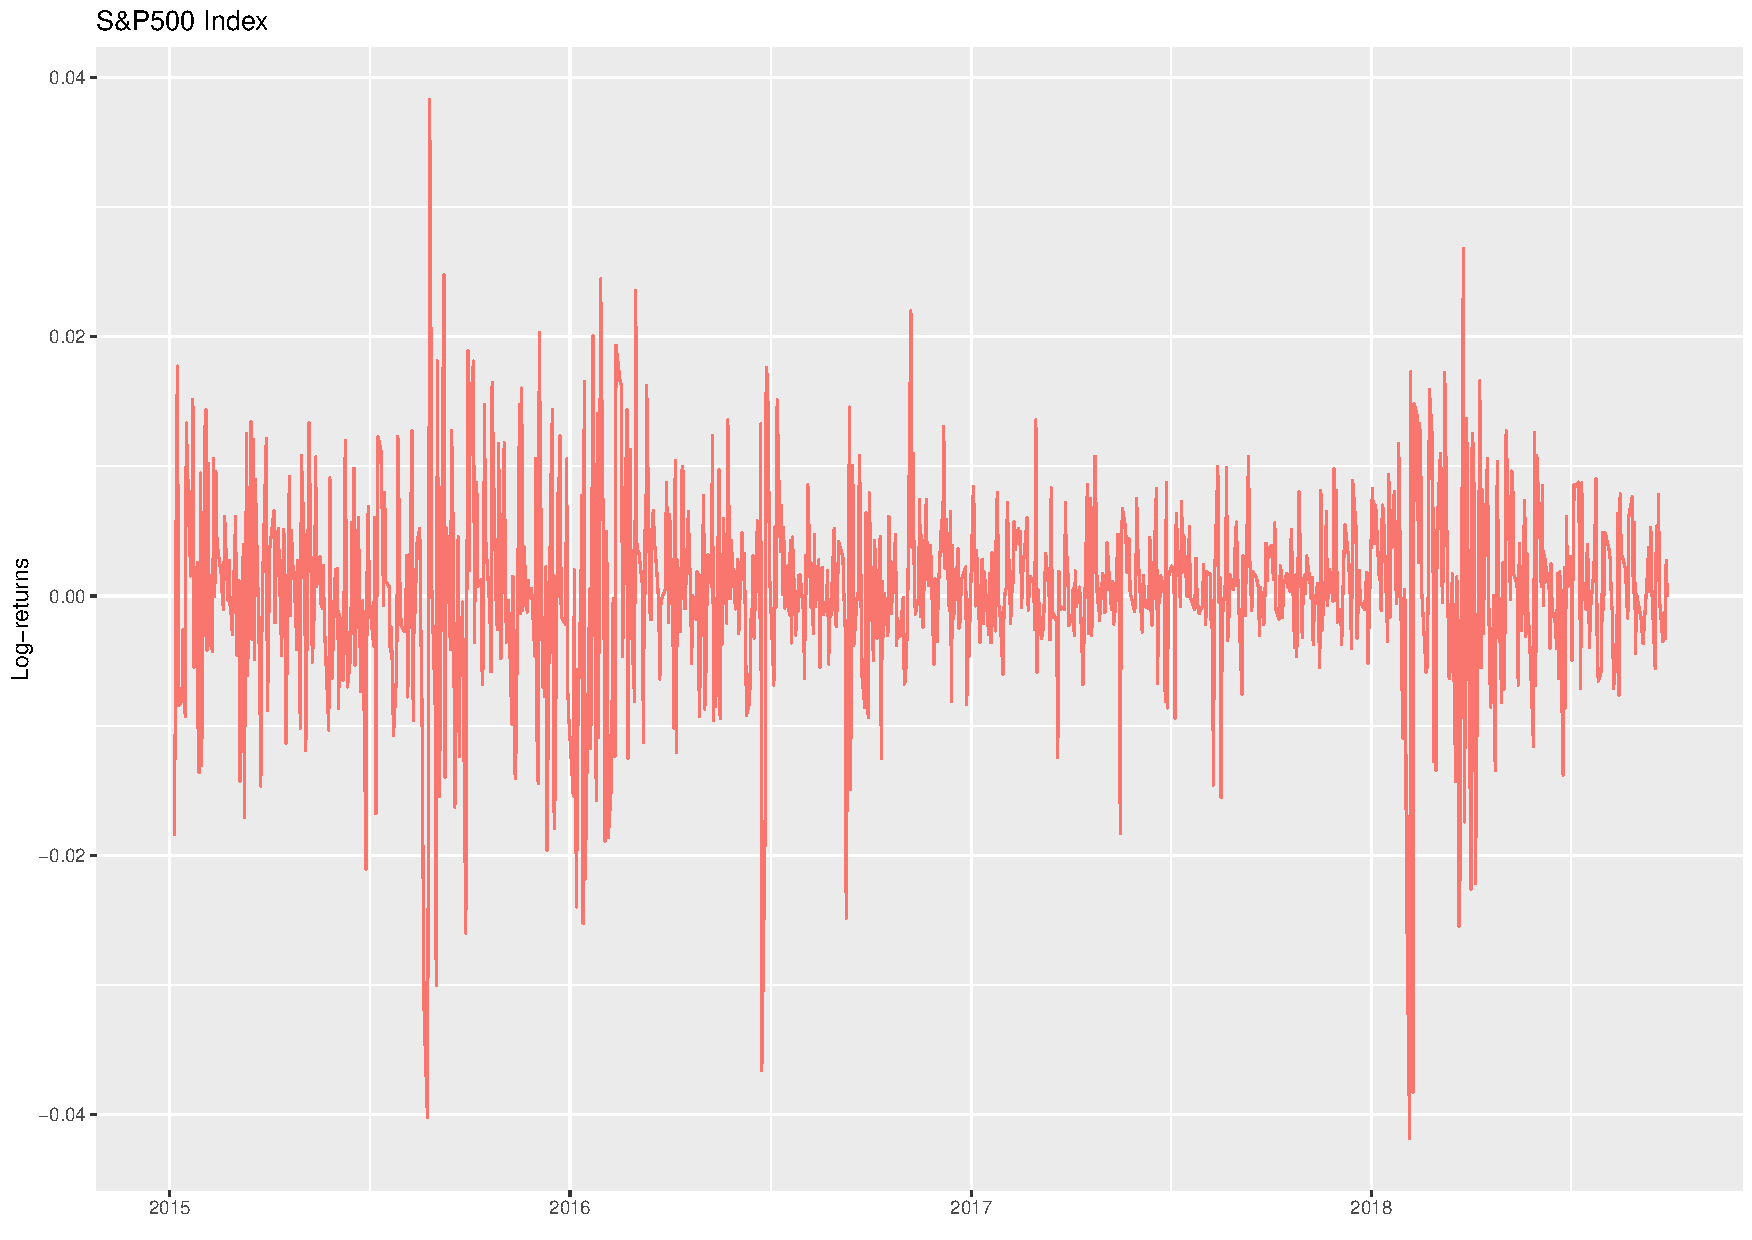
\includegraphics[scale=.25]{img/finData/logReturns}
		\caption{Log-Returns of the S\&P500}
		\label{fig:logReturnsSP500}
	\end{minipage}%
	\begin{minipage}{.5\textwidth}
		\centering
		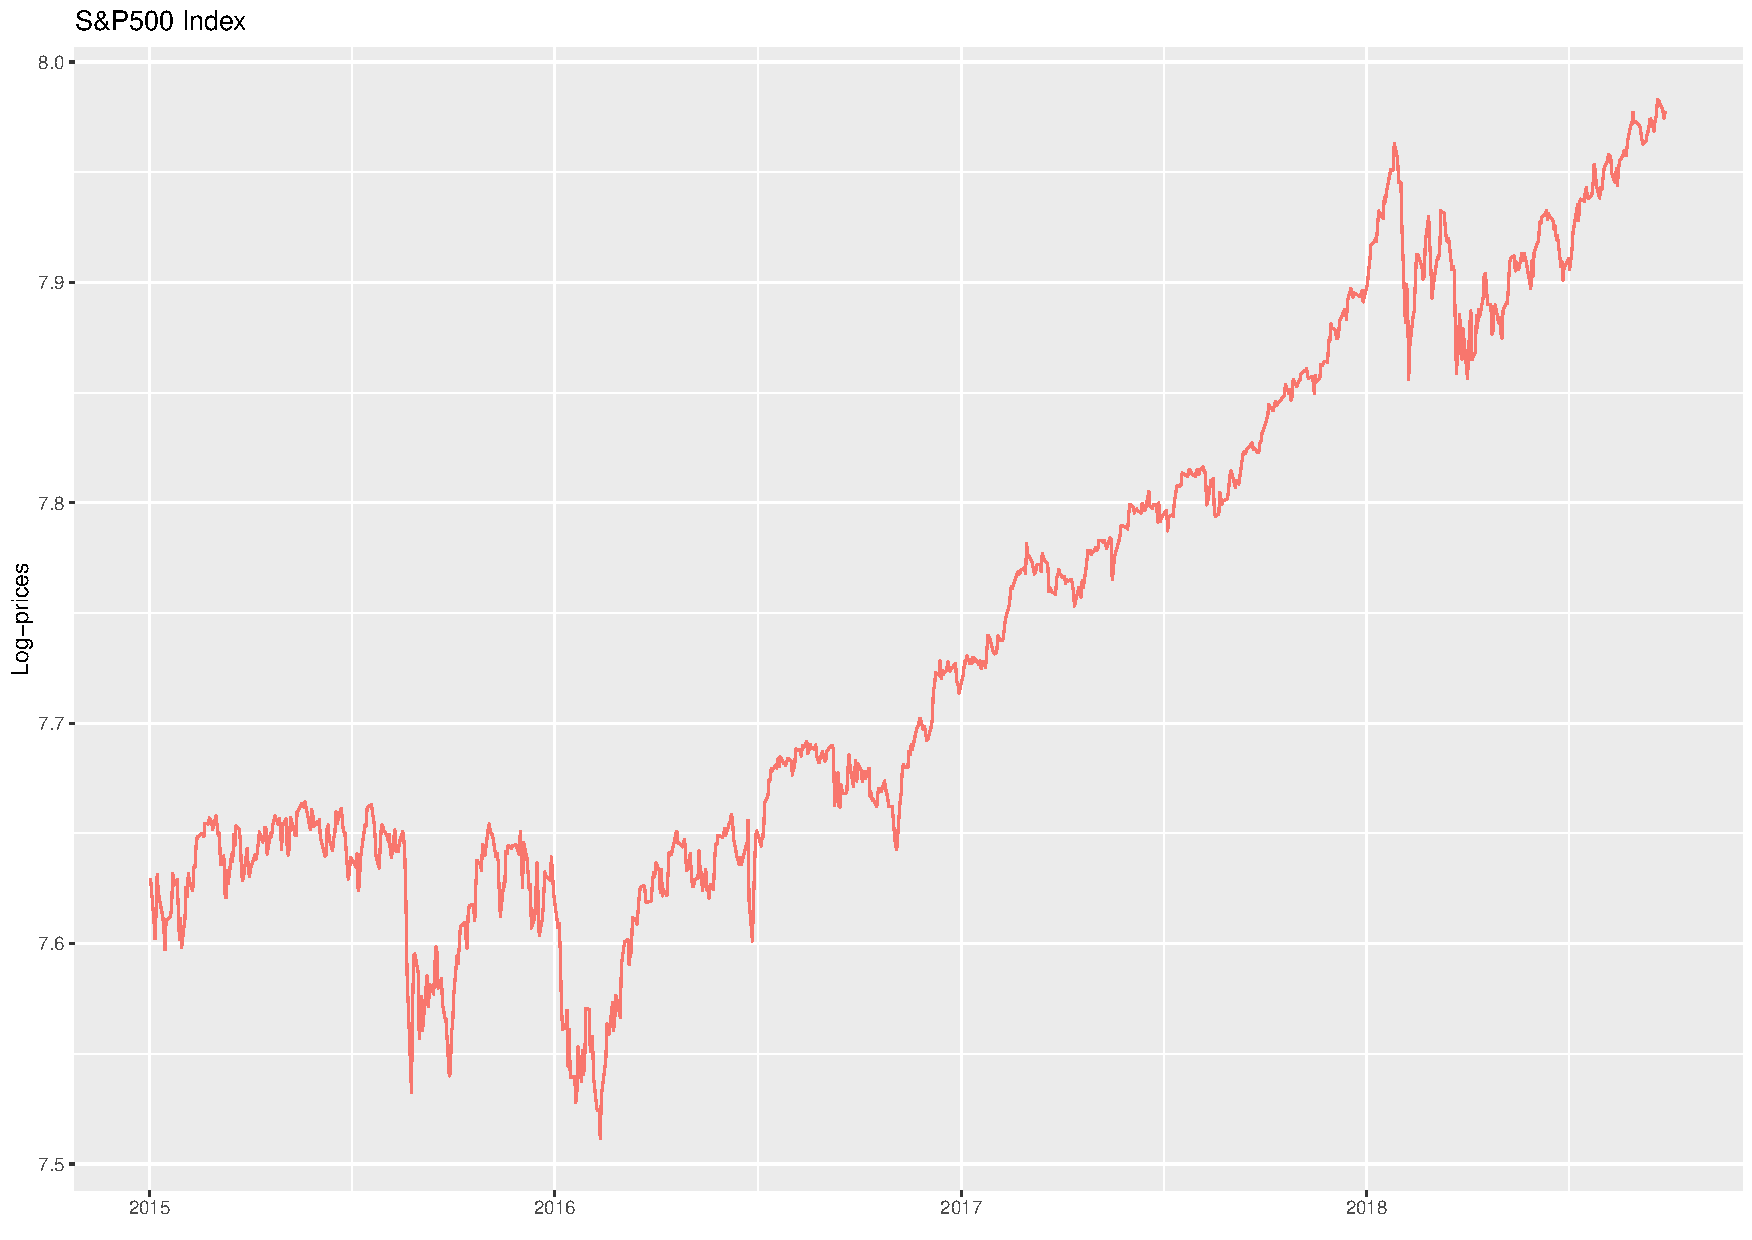
\includegraphics[scale=.25]{img/finData/logPrices}
		\caption{Log-Prices of the S\&P500}
		\label{fig:logPricesSP500}
	\end{minipage}
\end{figure}

\section{Stylized facts}
\label{sec:stylizedFacts}
In an attempt to portray financial data without the need of a theoretical 
framework, Rama Cont presents financial data in~\cite{stylizedFacts}. To 
introduce empirical properties he uses stylized facts, which are 
broad generalizations that summarize data.\\

In other words, this section will serve as a brief introduction to 
properties of financial data which have been observed in various types of 
financial markets. However, bear in mind that this is a first approximation 
and that stylized facts are not by any means facts.\\

With that being said, the stylized facts relevant to this work presented 
in~\cite{stylizedFacts} are:

\begin{enumerate}
	\item \textbf{Absence of autocorrelations:} linear autocorrelations of 
	asset returns are insignificant, except for small intraday scales. See 
	figure \ref{fig:acfDailyLogRet} for the autocorrelations of daily 
	S\&P500 log-returns.
	
	\item \textbf{Heavy tails:} The pdf of returns is heavy-tailed. That is, 
	its tails fall much slower than a Normal pdf, which falls exponentially 
	to zero.
	
	\item \textbf{Gain/loss asymmetry:} Extreme down movements are far more 
	common than huge upswings.
	
	\item \textbf{Aggregational Gaussianity:} The probability density 
	function (pdf) of log-returns approaches the one of a Gaussian random 
	variable as one increases the time scale over which returns are 
	calculated (see figure \ref{fig:HistLogRet}).
	
	\item \textbf{Intermittency:} Regardless of the time scale, returns 
	display high variability.
	
	\item \textbf{Volatility clustering:} As it can be seen in figure 
	\ref{fig:logReturnsSP500}, high volatility (dispersion of log-returns) 
	events tend to come in clusters.
\end{enumerate}


%\cite{stylizedFacts, AdvFML}

\section{Statistical properties}
In figure \ref{fig:acfDailyLogRet} one can see the autocorrelations of daily 
log-returns. The definition, as in~\cite{acfDefinition}, of the 
log-returns autocorrelation of lag $k$ is the following:

\begin{equation*}
	\rho_k = \frac{\text{Cov}(r_t, r_{t + k})}{\sqrt{\text{Var} [r_t]}
	\sqrt{\text{Var} [r_{t + k}]}}
\end{equation*} 

Where $\text{Cov}(r_t, r_{t + k})$ is the covariance of $r_t$ and 
$r_{t + k}$ and $\text{Var}[r_t]$ the variance of $r_t$.\\

It can be seen that, by definition, $\rho_0 = 1$. Apart from that, the rest 
of lags are insignificant or barely surpass the significant threshold 
(dotted line). This confirms the first stylized fact presented in section 
\ref{sec:stylizedFacts}.

\begin{figure}[hbtp]
	\centering
	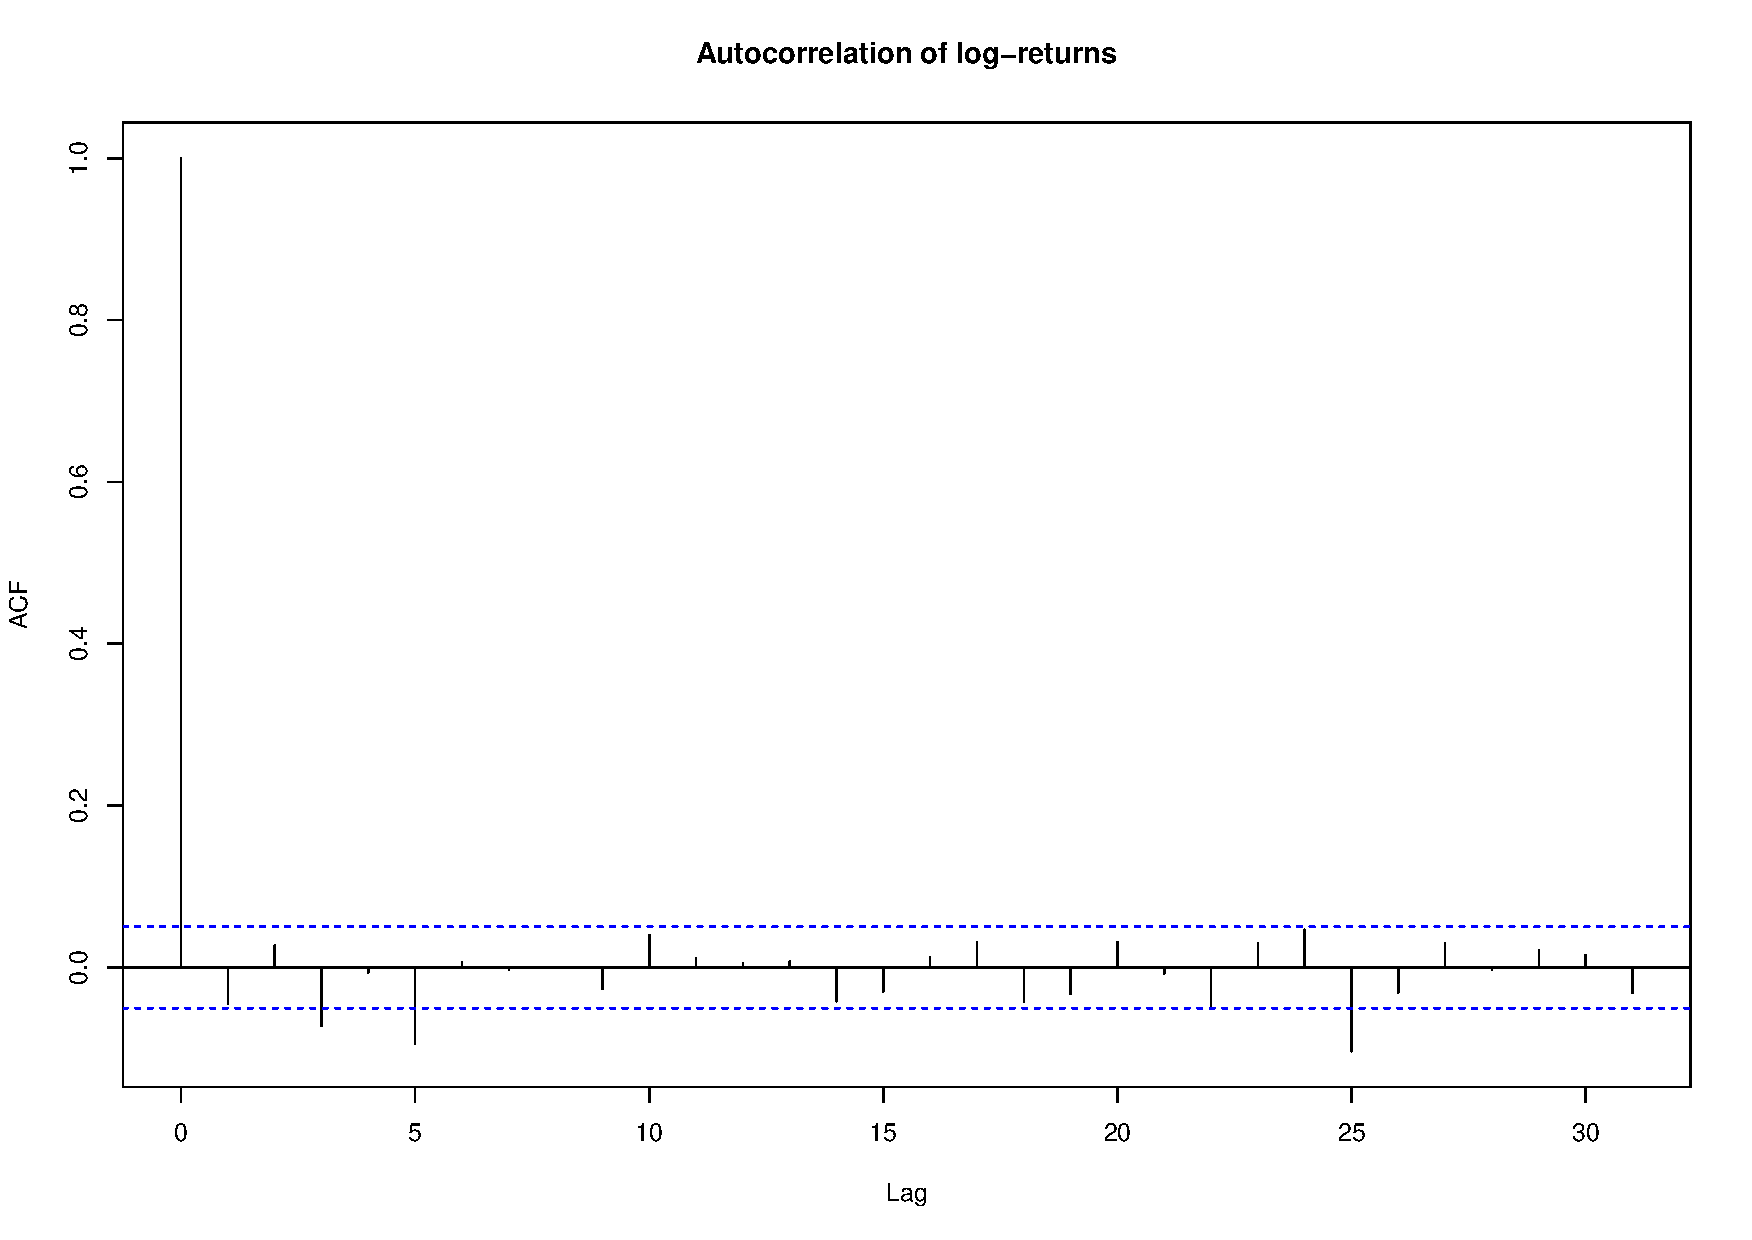
\includegraphics[scale=0.35]{img/finData/acfDailyLogRet}
	\caption{Autocorrelations of daily S\&P500 log-returns}
	\label{fig:acfDailyLogRet}
\end{figure}

Figure \ref{fig:HistLogRet} shows the histogram for daily, weekly and 
monthly log-returns of the S\&P500. It has been introduced with the 
intention of illustrating stylized facts 2 and 4. It clearly shows the heavy 
tails and how it evolves towards a normal distribution as the returns time 
scale increases.\\

\begin{figure}[hbtp]
	\centering
	\begin{subfigure}{.5\textwidth}
		\centering
		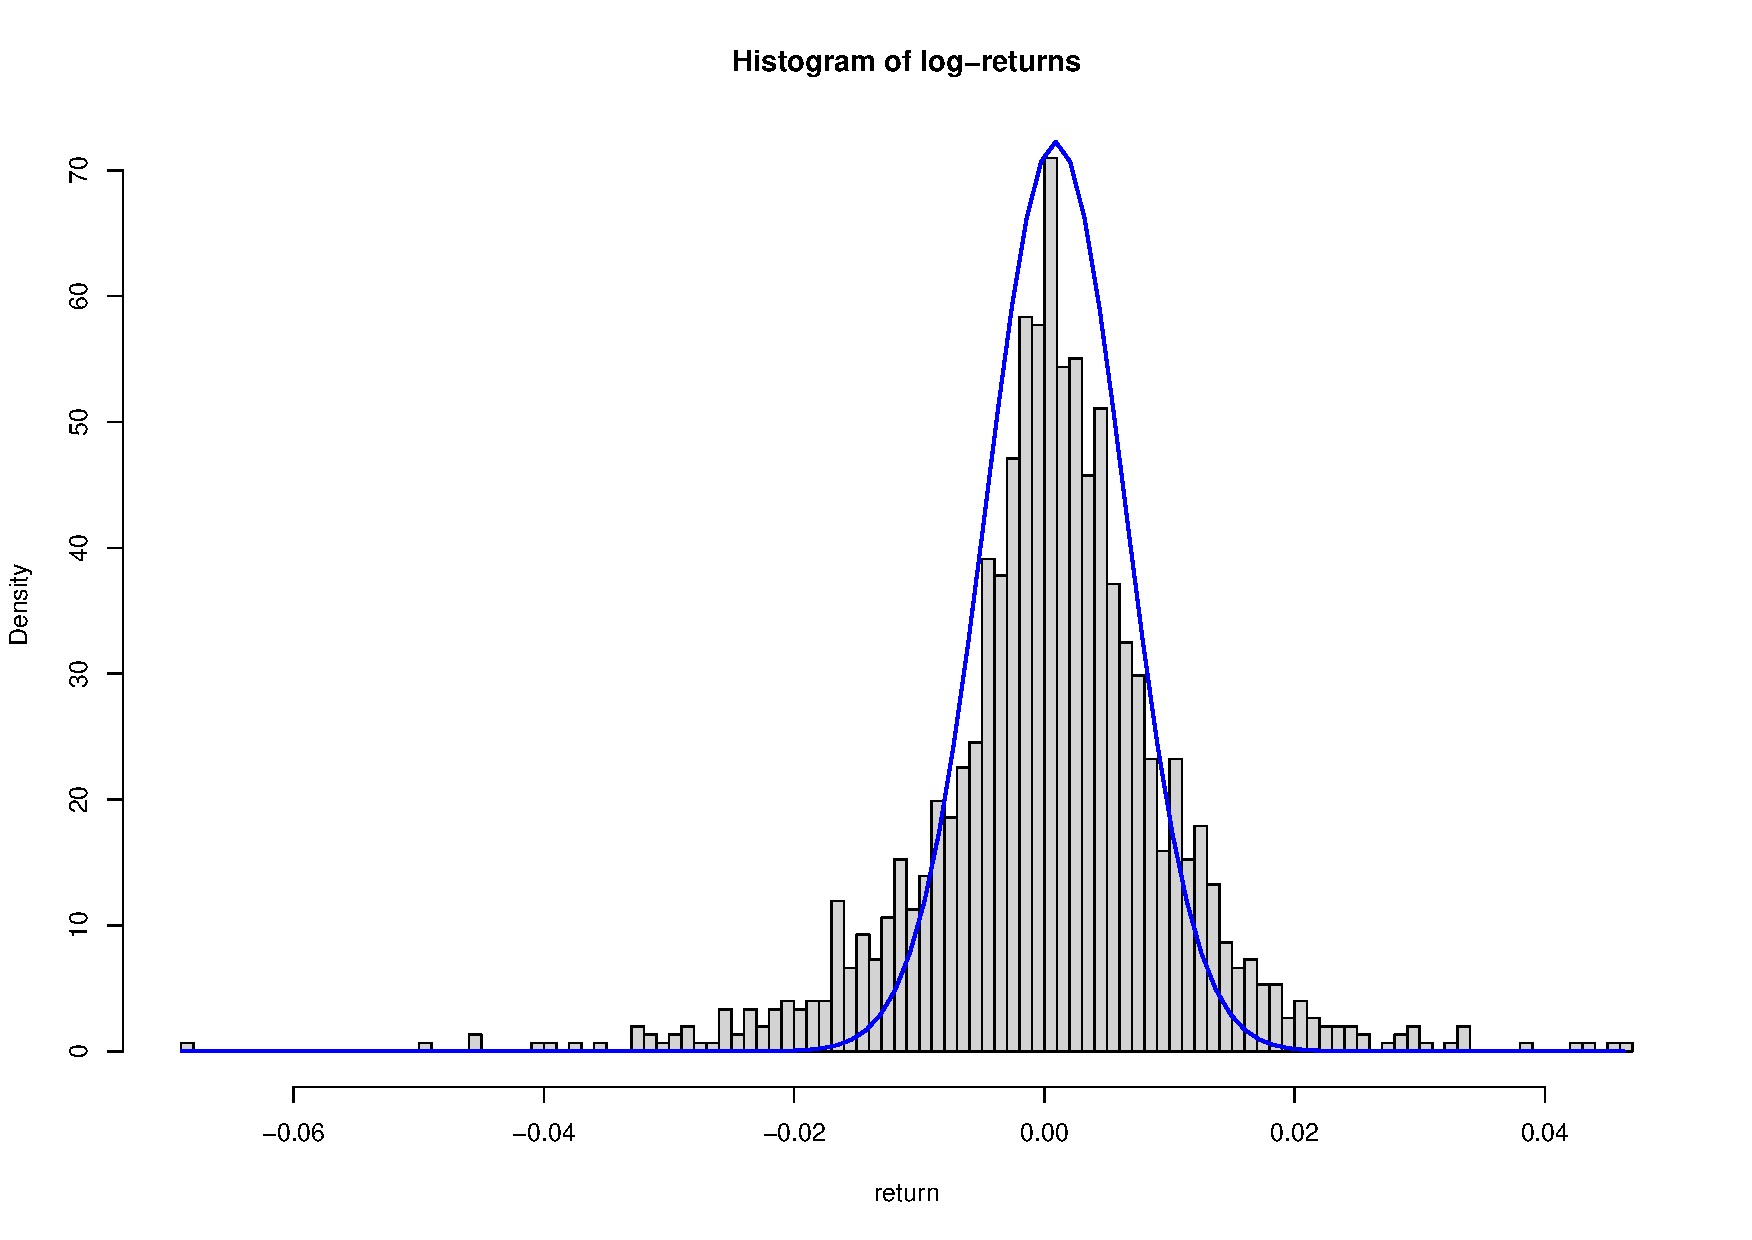
\includegraphics[scale=.2]{img/finData/histDailyLogRet}
		\caption{Daily log-returns}
	\end{subfigure}%
	\begin{subfigure}{.5\textwidth}
		\centering
		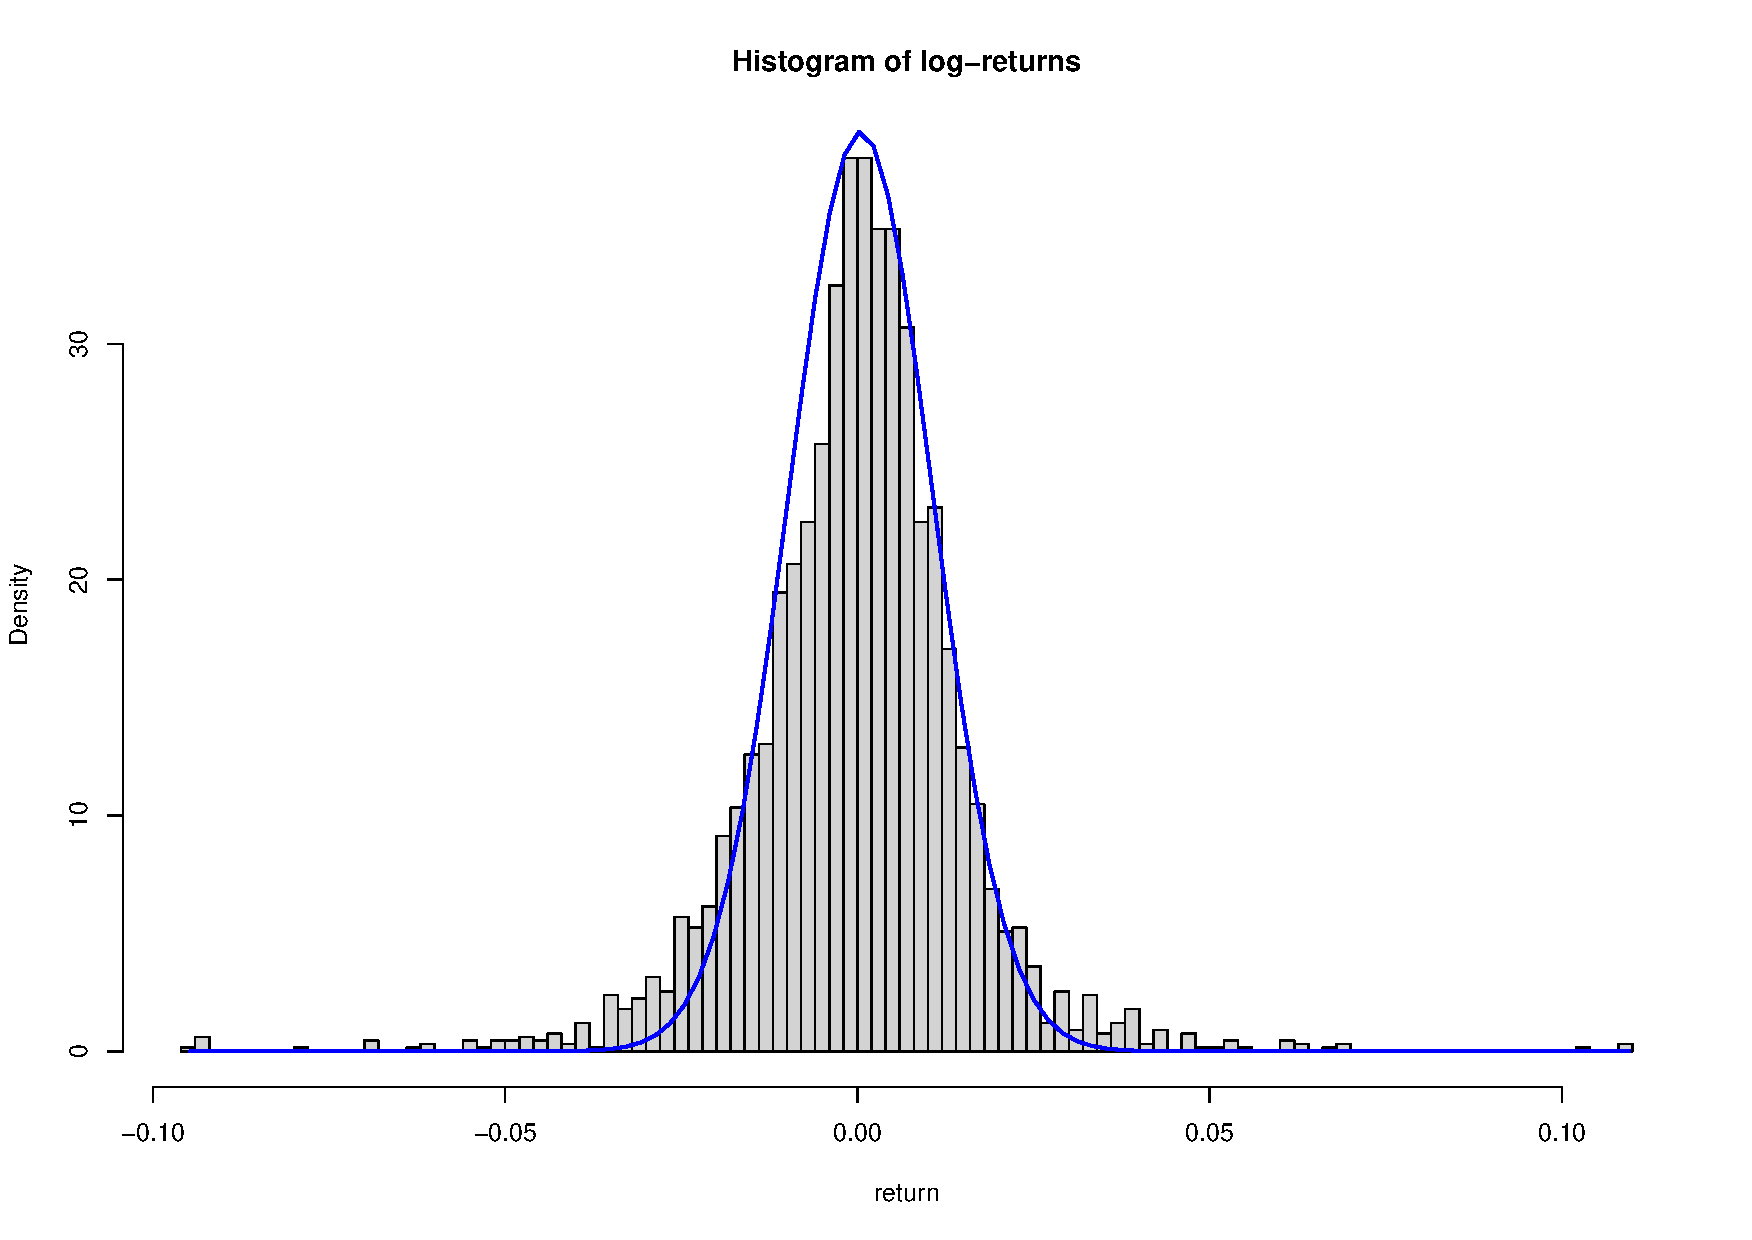
\includegraphics[scale=.2]{img/finData/histWeeklyLogRet}
		\caption{Weekly log-returns}
	\end{subfigure}
	
	\vspace{.4cm}
	
	\begin{subfigure}{\textwidth}
		\centering
		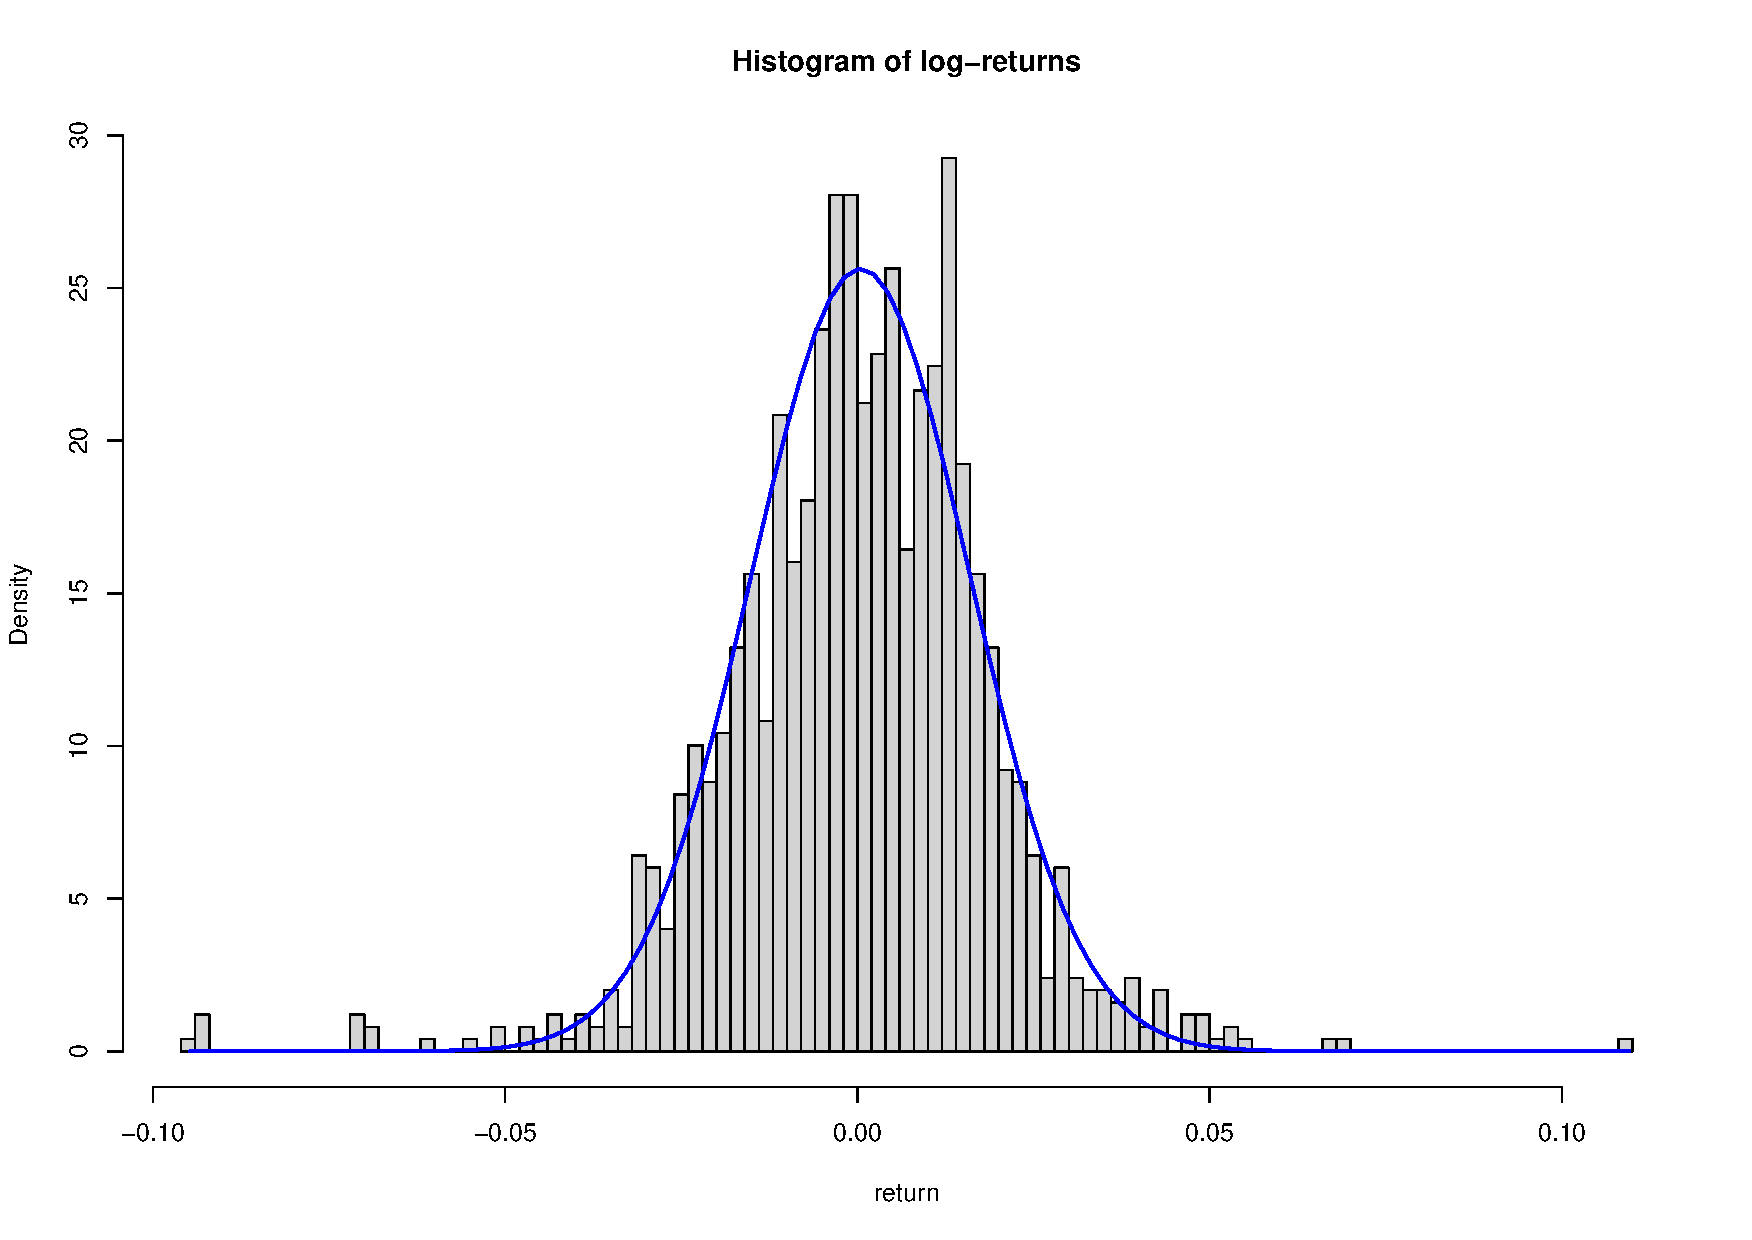
\includegraphics[scale=.2]{img/finData/histMonthlyLogRet}
		\caption{Monthly log-returns}
	\end{subfigure}
	
	\caption{Pdf fitted to S\&P500 log-returns}
	\label{fig:HistLogRet}
\end{figure}

Lastly, figure \ref{fig:QQPlotLogRet} illustrates, via QQ (Quantile 
Quantile) plots, that log-returns do not follow a normal distribution. 
Beforehand, it is pertinent to introduce special notation for quantiles:
given a r.v. X, a \textbf{quantile} $q_\alpha$ is a real number s.t. $P(X 
\leq q_\alpha) = \alpha$\\

That said, Quantile Quantile plots order the observations, and then map them 
to the graph such that the value of the x-axis is the equivalent quantile of 
$Z \sim N(0,1)$, and the value of the y-axis is the quantile of the sample. 
That way, if one wants to test if $X \sim N(\mu, \sigma^2)$, then knowing 
that the quantiles would just be shifted and/or scaled, the corresponding QQ 
Plot should be a line.\\

In the case of the S\&P500 log-returns (see figure \ref{fig:QQPlotLogRet}), 
the QQ Plots are not lines, implying that log-returns are not Normal. In 
addition, the curvature at the extremes is a clear sign of a heavy-tailed 
distribution.

\begin{figure}[hbtp]
	\centering
	\begin{subfigure}{.5\textwidth}
		\centering
		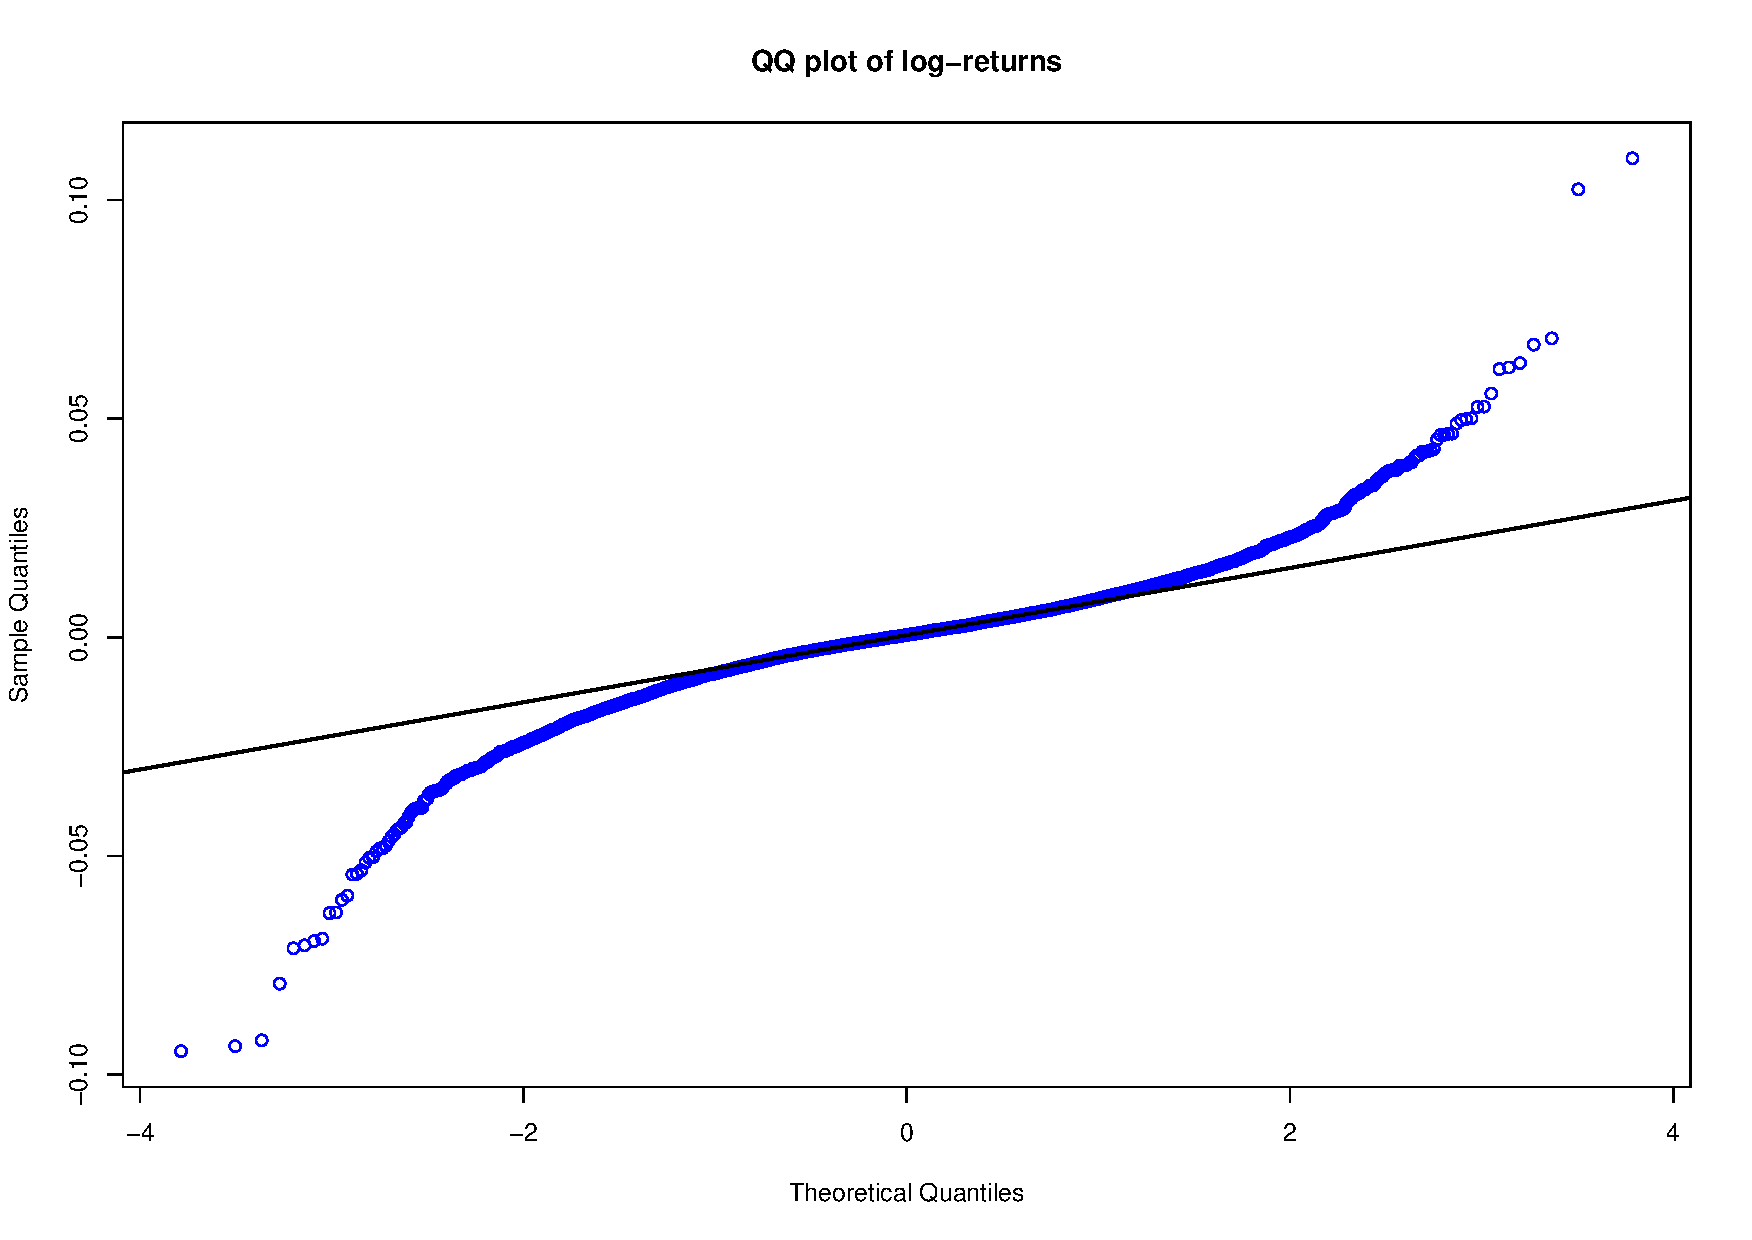
\includegraphics[scale=.2]{img/finData/QQPlotDailyLogRet}
		\caption{Daily log-returns}
	\end{subfigure}%
	\begin{subfigure}{.5\textwidth}
		\centering
		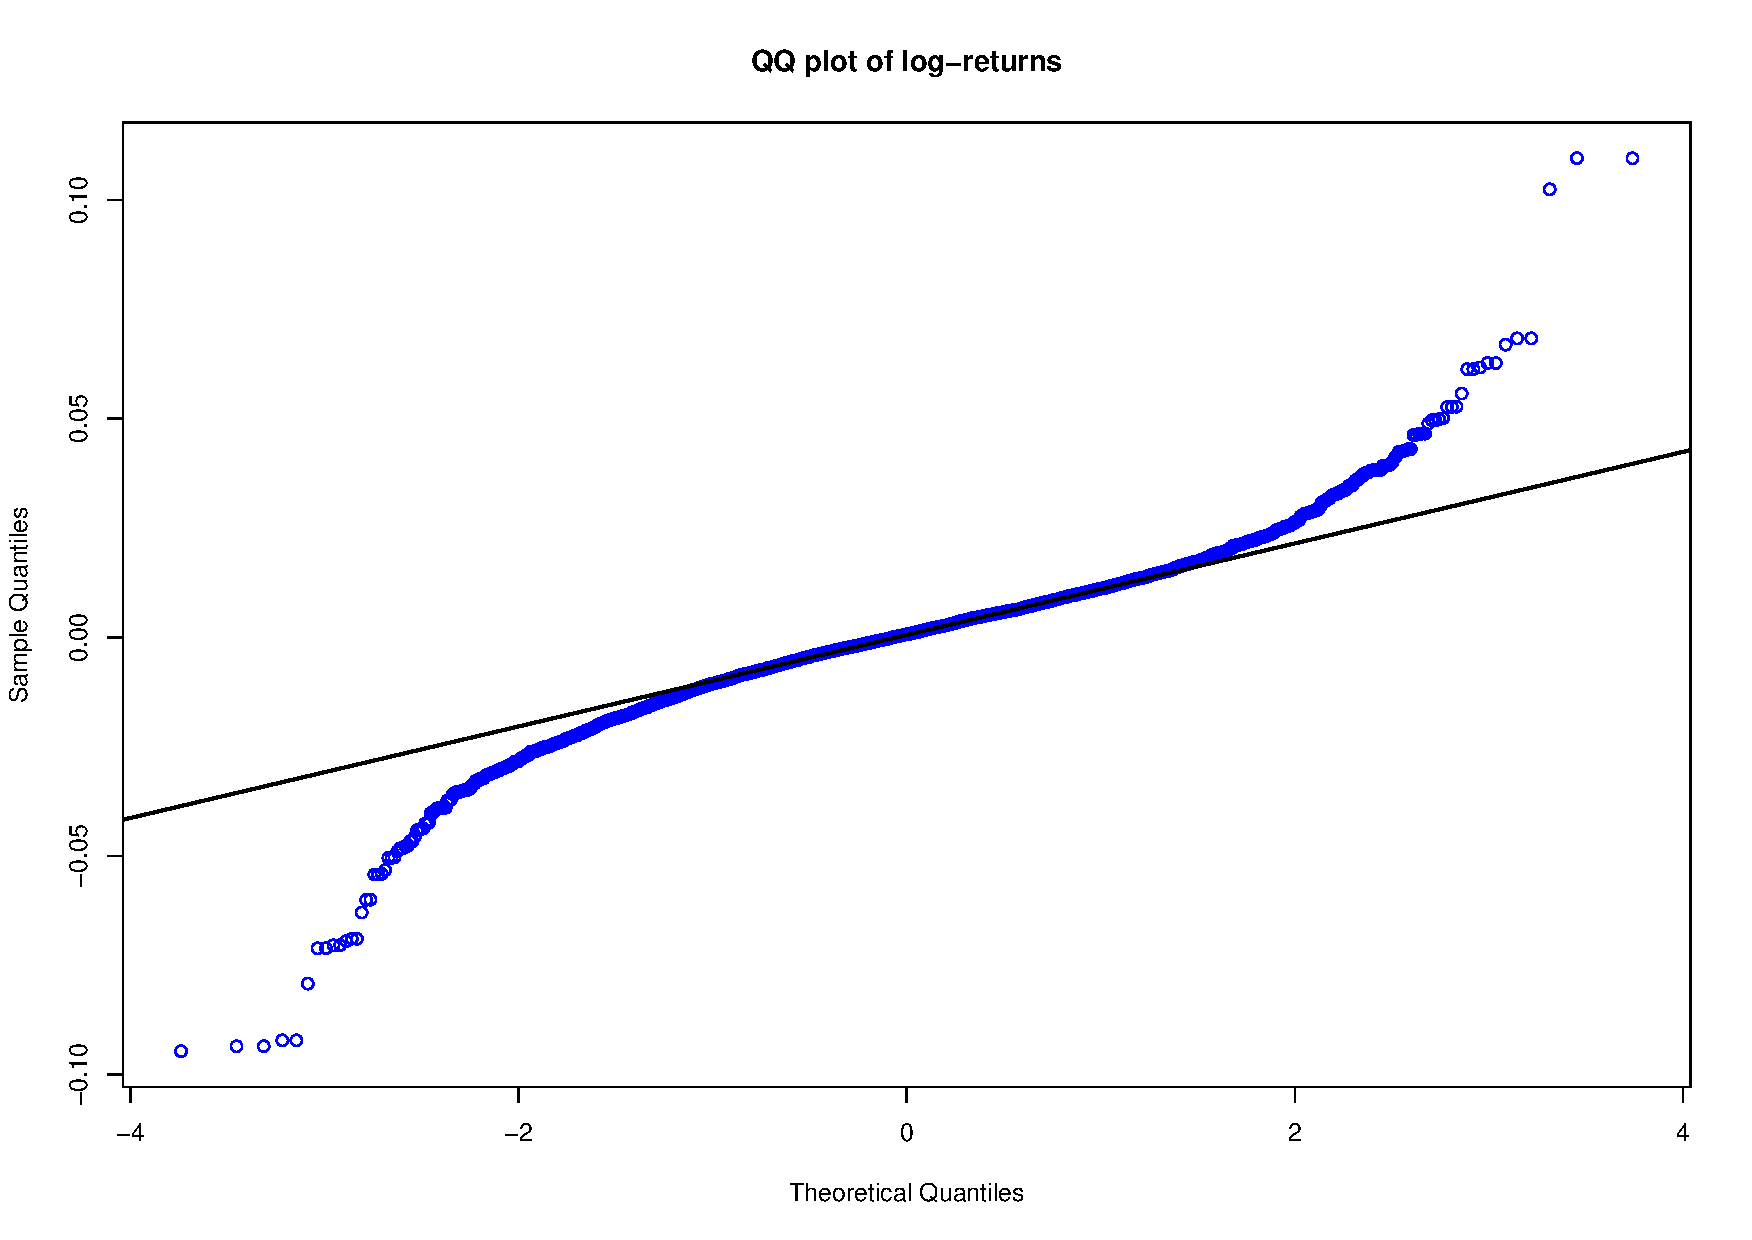
\includegraphics[scale=.2]{img/finData/QQPlotWeeklyLogRet}
		\caption{Weekly log-returns}
	\end{subfigure}%
	
	\vspace{.4cm}
	
	\begin{subfigure}{\textwidth}
		\centering
		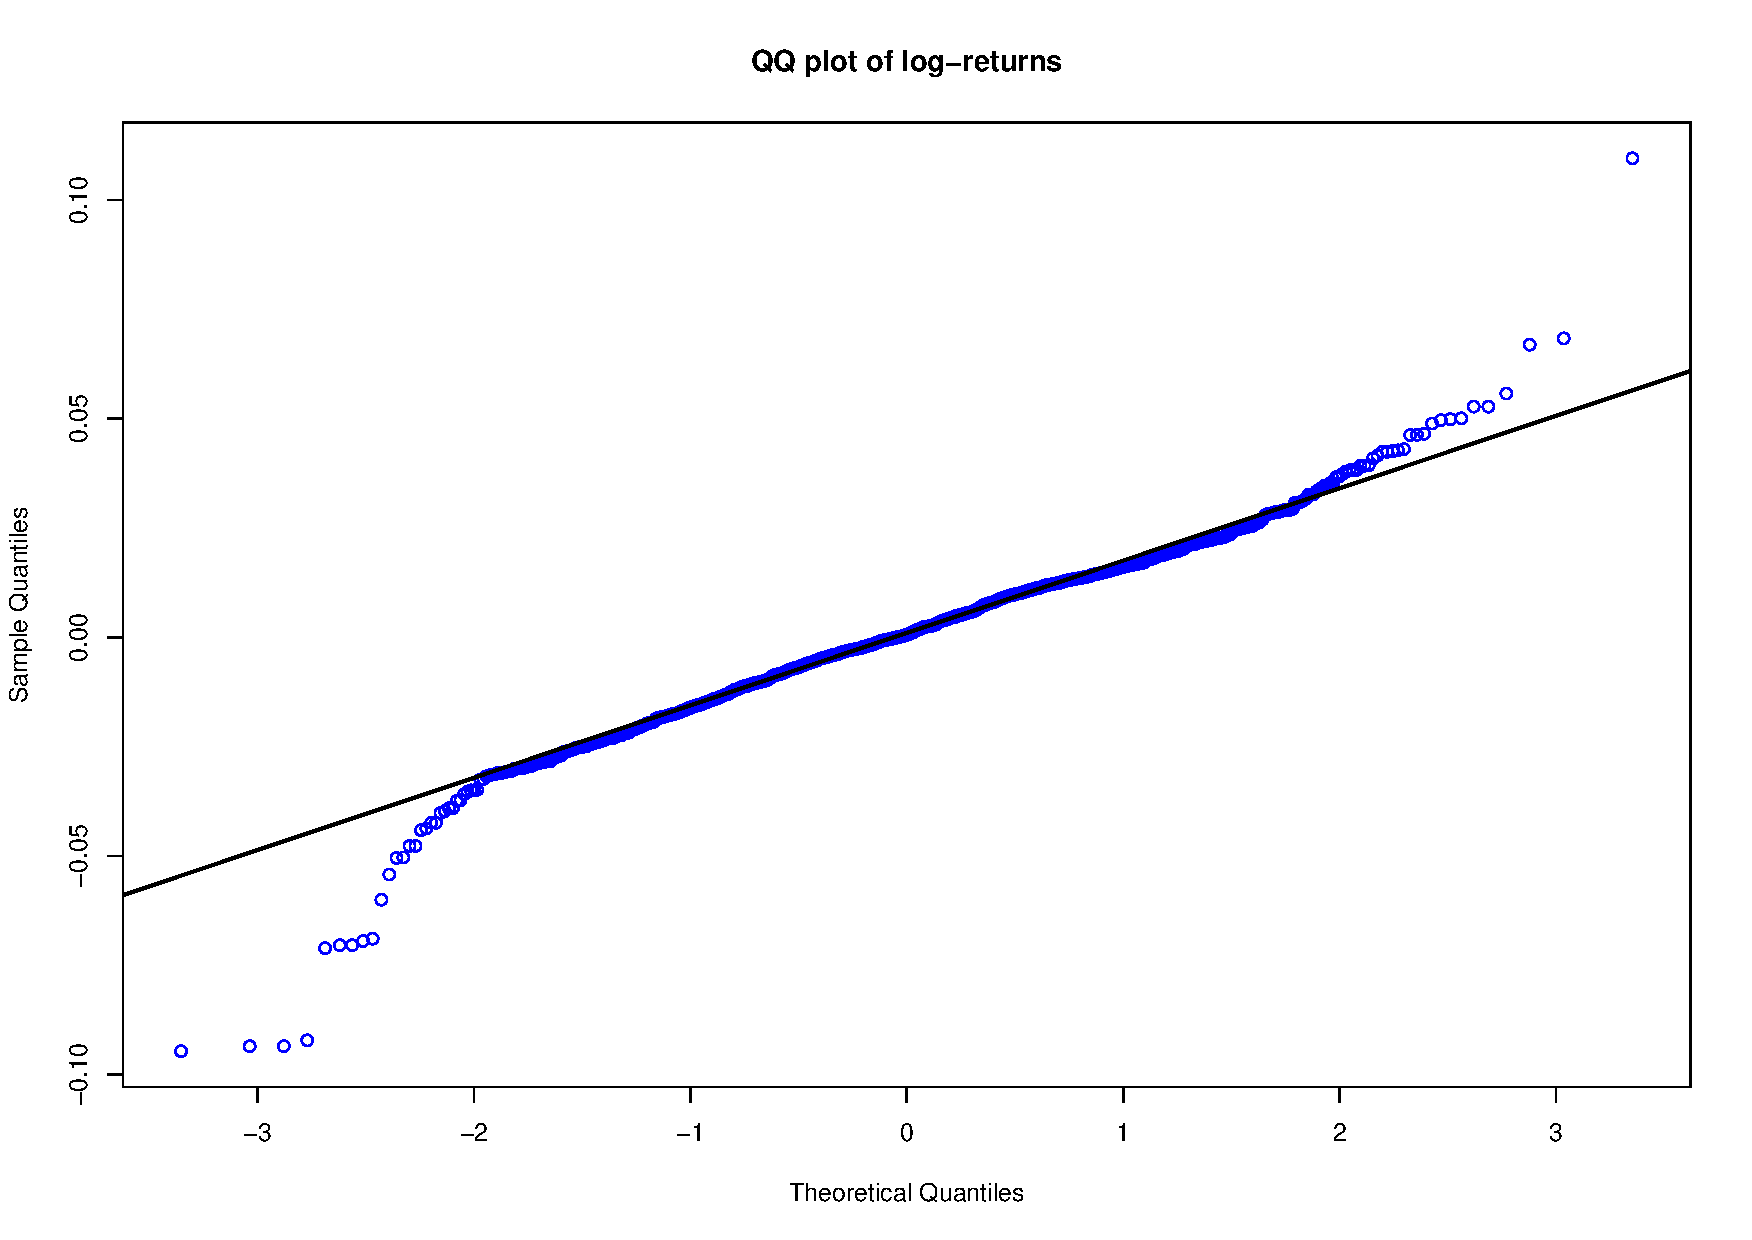
\includegraphics[scale=.2]{img/finData/QQPlotMonthlyLogRet}
		\caption{Monthly log-returns}
	\end{subfigure}
	
	\caption{QQ Plots of S\&P500 log-returns}
	\label{fig:QQPlotLogRet}
\end{figure}

\newpage

\section{Portfolios}
This section will introduce the concept of portfolios, which essentially 
means that one can allocate a certain budget to different financial products 
instead of buying a single asset. In this work, $N$ will represent the 
number of securities and $\mathbf{w} \in \mathbb{R}^N$ the vector of weights 
assigned to each asset. Accordingly, the price of each stock considered in 
the portfolio will be noted as $p_t^i$, where $i \in \{1,\ \ldots ,\ N\}$.\\

Regarding notation for portfolio returns it is useful to set the following 
terms:
\begin{itemize}
	\item \textbf{Money available (budget):} $B$
	
	\item \textbf{Portfolio linear returns:}  $R_t^P$
	
	\item \textbf{Portfolio log-returns:} $r_t^P$
	
	\item \textbf{Linear returns of asset $i$}: $R_t^i \longleftrightarrow
	\textbf{R}_t = [ R_t^1 ,\ \ldots ,\ R_t^N ]$
	
	\item \textbf{Log-returns of asset $i$}: $r_t^i \longleftrightarrow 
	\textbf{r}_t = [ r_t^1 ,\ \ldots ,\ r_t^N ]$
\end{itemize}

Recognizing that the amount of money invested in asset $i$ is simply 
$B w_i$, $R_t^P$ can be computed as:
\begin{align*}
	R_t^P = \frac{\sum_{i = 1}^{N} B w_i \cdot (1 + R_{t}^{i})}{B} - 1 =
	\sum_{i = 1}^{N} (w_i + w_i \cdot R_{t}^{i}) - 1 =
	\textbf{w} \cdot \textbf{R}_{t}\\
	r_t^P = \log (1 + R_t^P)\hfill
\end{align*}

Where it has been used that:
\begin{itemize}
	\item $\sum_{i=1}^N w_i = 1$ because in the cases that are going to be 
	considered there is no leverage. This constraint just means that the sum 
	of the money invested in each asset is $B$
	
	\item If $B w_i$ is the initial wealth of asset $i$ at time $t-1$, then 
	the final wealth is $B w_i \cdot (1 + R_t^i) = B w_i \cdot 
	\frac{p_t^i}{p_{t-1}^{i}}$
\end{itemize}

\section{Long and short positions}
When opening a position it is really important to distinguish between long
and short positions. A long position (or going long on some stock) is the 
most common way to invest since it just means that you buy an asset and you 
sell it at some point, expecting to earn a return.\\

On the contrary, if you short a stock, you first sell a stock that someone 
has lent you and then try to repurchase it at a lower price to return the 
stock to the lender. That way, if the stock goes down in price, you would 
earn a profit by selling high and buying low.\\

The following examples will attempt to clarify what was mentioned before:
\subsection*{Long position}
Suppose the prices of stock \textbf{ABC} at times $t_0$ and $t_1 := t_0 + 1$ 
are $p_{t_0} = 100\$ $ and $p_{t_1} = 115\$ $ respectively. Then, the return 
is: $R_{t_1} = \frac{115}{100} - 1 = 0.15$. If at $t_0$ one buys 10 stocks 
of \textbf{ABC} at market value ($B = 10 \cdot p_{t_0} = 1000\$ $), the end 
wealth at $t_1$ will be $B \cdot (1 + R_{t_1}) = 1150\$ $. Thus, the final 
profit has been 150\$.\\

Conversely, if the stock would have gone down in price at time $t_1$, money 
would have been lost. At this point, it is obvious that long positions will 
only be profitable if the stock price ends at a higher value than the one 
when the position was opened.

\subsection*{Short position}
Following the example of the long position, suppose that at time $t_0$ one 
shorts 10 stocks of \textbf{ABC}. That means that 10 stocks will be lent to 
us to be sold immediately at market value, making one hold 1000\$ in cash.\\

As the stock at time $t_1$ has gone up in value, one repurchases the shares 
at 1150\$, realizing a 150\$ loss. However, if at time $t_1$ the stock price 
would have been $p_{t_1} = 85\$ $, then the stocks would have been 
repurchased at 850\$, realizing a 150\$ profit. From a practical standpoint, 
the end wealth of a short position can be calculated as 
$B \cdot (1 - R_{t_1})$ since:

\begin{equation*}
	R_{t_1}^{\text{short}} = \frac{\text{profits}}{p_{t_0}} =  
	\frac{p_{t_0} - p_{t_1}}{p_{t_0}} = - R_{t_1}
\end{equation*}

where \textbf{profits} means the money you would earn if you shorted one 
stock (selling at $p_{t_0}$ and buying at $p_{t_1}$) and 
$R_{t_1}^{\text{short}}$ the return realized at $t_1$ by shorting one stock 
at $t_1$.\\

As a final note, it should be pointed out that shorting a stock can lead to 
ever-growing losses. This is caused by the definition of shorting, which 
implies receiving stocks from someone who expects them back. So if a stock 
keeps going up in price, then the stocks will be repurchased at a price that 
will keep growing. On the other hand, if one goes long on a stock, the 
maximum capital that can be lost is the initial one, which would only happen 
if the stock price went to 0.

\section{Financial Metrics}
In this section, a series of financial metrics will be shown so as to 
compare results in the succeeding chapters:
\begin{itemize}
	\item Sharpe Ratio
	\item Information Ratio
	\item Drawdown
\end{itemize}

\subsection*{Sharpe Ratio}
The Sharpe ratio is extremely useful since it allows to compare assets 
independent of the returns and variability. This metric, as defined by 
William F. Sharpe in \cite{sharpe1994sharpe}, was introduced with the
concept of reward per unit of variability in mind:
\begin{equation}
	\label{eqn:williamFSharpe}
	\text{SR} = \frac{\mathbb{E}[R_t - r_f]}{\sqrt{\text{Var}[R_t - r_f]}}
\end{equation}

The term $r_f$ in equation \ref{eqn:williamFSharpe} is the risk-free return, 
which is the rate of return you can achieve with zero risk. An example of 
this is the 1 month U.S. Treasury bills. As a side note, the term $r_f$ was 
introduced because assets carrying risk must surpass $r_f$ to encourage 
investors to buy them.

\subsection*{Information Ratio}
Similarly to the Sharpe Ratio, the Information Ratio is useful to compare 
the returns achieved with a benchmark:

\begin{equation*}
	\label{eqn:informationRatio}
	\text{IR} = \frac{\mathbb{E}[R_t - R_b]}{\sqrt{\text{Var}[R_t - R_b]}}
\end{equation*}
Where $R_b$ are the returns of the benchmark, $\alpha := \mathbb{E}[R_t - 
R_b]$ is the excess return, and $\sqrt{\text{Var}[R_t - R_b]}$ is one of the 
many definitions of tracking error.

\subsection*{Drawdown}
The drawdown of an investment at time $t$ is noted as $D(t)$ and is a 
risk-related metric that measures the relative drop from a historical peak 
(High Water Mark):
\begin{equation*}
	D(t) = \frac{\text{HWM}(t) - p_t}{\text{HWM}(t)}
\end{equation*}

Where 

\begin{equation*}
	\text{HWM}(t) = \max_{1 \leq \tau \leq t} p_t
\end{equation*}

\section{High Frequency Data}
\label{sec:highFrequencyData}
The purest form of financial data is called tick data, which collects the 
information of sellers and buyers of a financial product. The way traders 
enter the market is by posting \textbf{orders}, that can be either 
\textbf{buy or sell orders}. A buy (sell) order represents the will of a 
trader to buy (sell) $m$ units of an asset at a price $p$.\\

Before giving an overview of tick data, a few concepts should be defined:
\begin{itemize}
	\item \textbf{Bid price} ($b_t$): maximum price out of all the buy 
	orders at time $t$.
	
	\item \textbf{Ask price} ($a_t$): minimum price out of all the sell 
	orders at time $t$.
	
	\item \textbf{Mid price:} $m_t = \frac{a_t + b_t}{2}$
	
	%\item \textbf{Price:} ($p_t$) price of the last asset sold.
	
	%\item \textbf{Volume:} ($v_t$) number of stocks exchanged.
	
	\item \textbf{Tick size:} smallest change in price a stock can move 
	(e.g. 0.001\$).
\end{itemize}

Note that orders are ordered in price and time. This means that if one posts 
an order to sell 10 units of an asset at time \textbf{10:00:21} at a price 
of 10.00\$, then one would have less priority than a person that wanted to 
sell 4 units at time \textbf{10:00:18} at the same price.\\

Having said that, a few remarks follow:
\begin{enumerate}
	\item If one were to buy or sell \textbf{one unit} of an asset, it could 
	be done instantly at prices $a_t$ and $b_t$ respectively.

	\item If the tick size did not exist then traders could jump ahead by 
	increasing the bid or ask prices by a small amount $\epsilon$.
	
	\item The spread ($a_t - b_t > 0$) is a measure of the liquidity of the 
	asset in question. That is, how buyers and sellers agree.
	
	\item Data is \textbf{inhomogenous} in the sense that it does not arrive 
	at fixed time intervals (see table \ref{tab:tickData}). In fact, only 
	when agreements are made between buyers and sellers will a new tick be 
	recorded. Therefore, in a period of high activity a lot of 
	\textbf{ticks} ($\{t, p_t, b_t, a_t, v_t \}$) will be recorded in a 
	short time span, and vice versa.
\end{enumerate}


\begin{table}[htbp]
\caption{Example of tick data}
\label{tab:tickData}
\centering
\begin{tabular}{ |C{5cm}|C{2cm}|C{2cm}|C{2cm}|C{2cm}| }
	\hline
	$t$ & $p_t$ & $b_t$ & $a_t$ & $v_t$\\
	\hline
	2013-01-02 08:00:00 & 67.18 & 67.18 & 67.78 & 125\\
	2013-01-02 08:12:56 & 67.70 & 67.19 & 67.70 & 125\\
	2013-01-02 08:12:56 & 67.75 & 67.75 & 67.82 & 125\\
	2013-01-02 08:47:15 & 67.91 & 67.21 & 67.93 & 150\\
	2013-01-02 09:29:09 & 67.55 & 67.52 & 67.55 & 200\\
	2013-01-02 09:29:09 & 67.56 & 67.51 & 67.57 & 200\\
	2013-01-02 09:29:10 & 67.56 & 67.51 & 67.58 & 200\\
	2013-01-02 09:29:10 & 67.58 & 67.51 & 67.57 & 100\\
	2013-01-02 09:29:10 & 67.58 & 67.52 & 67.58 & 100\\
	2013-01-02 09:29:11 & 67.57 & 67.52 & 67.58 & 200\\
	\hline
\end{tabular}
\end{table}


\chapter{Meta-labeling}
\label{chapterMetaLabeling}

\section{Introduction}
\label{sec:intro}
Labeling is a well-known area in Machine Learning. It consists of gathering 
a matrix $X$, known as features, whose rows are the observations. Once a 
label $y_i$ is assigned to every row $X_{[i,\cdot]}$ the main goal is to give 
a prediction $\widehat{y}_i$. Whenever $y_i \in I$ s.t. $|I| = 2$, the 
problem can be referred as a binary classification one, which is what this 
chapter will focus on.\\

When it comes to Finance, labeling is not as straightforward as a 
conventional case, i.e. predicting deterministic events; yes/no traffic 
light in the picture, yes/no happy face, etc. Since one is working with 
returns, one needs to determine whether a positive (negative) outcome will 
happen (or not) in a determined time horizon.\\

The investment literature has tried to label observations using what Marcos 
López de Prado (MLDP) \cite{AdvFML} defines as \textit{The Fixed-Time 
Horizon Method}:

\begin{equation}
	y_i =
    \begin{cases}
      -1 & \text{if}\ r_{t_{i, 0} + h}(h) < \tau \\
      \hfill 0 & \text{if}\ |r_{t_{i, 0} + h}(h)| \leq \tau \\
      \hfill 1 & \text{if}\ r_{t_{i, 0} + h}(h) > \tau
    \end{cases}
\end{equation}

Where $r_{t_{i, 0} + h}(h)$ is the log-return from time $t_{i, 0}$ to 
$t_{i, 0} + h$ (in this case, $h$ is a time bar that can be days, months, 
etc.).\\

The problem with computing labels with a fixed threshold $\tau$ is that 
volatility, $\sigma$, changes overtime and should be updated regularly. Apart 
from that, restricting the model to a fixed $h$ is not optimal at all since 
more flexible ways can be implemented.

\section{Motivation}
\label{sec:motiv}
A portfolio of $N$ securities is defined by the weights, $\textbf{w} 
\in \mathbb{R}^N$ it gives to every instrument. In order to minimize 
the volatility, the Global Minimum Variance portfolio (\textbf{GMVP}) 
is defined as:

\begin{equation}
	\begin{aligned}
		\min_{w} \quad & w^{T} \mathbf{\Sigma} w\\
		\textrm{subject to} \quad & w \geq 0\\
 		 & \sum_{i = 1}^{N} w_i = 1    \\
	\end{aligned}
\end{equation}

Where $\mathbf{\Sigma}$ is the Covariance matrix of the $N$ stock's log-
returns.\\

At this point, remembering that the portfolio returns can be calculated as 
$\textbf{w} \cdot \mathbf{R_{t}}$, it is appropriate to talk about a 
single time series. In other words, the portfolio indirectly 
transforms a multivariate time series into a univariate one. 
Consequently, from now on, only the portfolio time series will be 
analyzed.\\ 

Regarding the motivation, as it can be seen in figure \ref{fig:GMVP_fall}, 
the falls in late 2018 and early 2020 are a huge setback as far as the final 
wealth is concerned. Going back to section \ref{sec:intro}, the general idea 
is to label these periods accordingly so that these drawdowns can be 
predicted.\\

\begin{figure}[htbp]
	\centering
	\includegraphics[scale=.3]{"\homeCOne/img/GMVP_fall"}
	\caption{GMVP portfolio prices}
	\label{fig:GMVP_fall}
\end{figure}

\section{What is meta-labeling?}
In this chapter the concept of meta-labeling will be introduced using the 
diagram found in figure \ref{fig:metaLabelingDiagram}, adapted from 
\cite{metaLabelingSignalEfficacy}.

\begin{figure}[htbp]
	\centering
	\includegraphics[width=.8\textwidth]
	{"\homeCOne/img/metaLabelingDiagram2"}
	\caption{Meta-labeling model diagram}
	\label{fig:metaLabelingDiagram}
\end{figure}

Bet-sizing is a common problem within the practitioner scene. That is, 
investors often know the side of the position they want to open (long/short 
or pass) but the size is unknown to them. Hence, an exogenous model that 
could base its predictions on some features, and the side prediction, comes 
into play.\\

The basic idea behind meta-labeling is having two models:
\begin{itemize}
	\item \textbf{Primary Model:} in charge of determining whether one 
	should open a long or short position on a given day.
	
	\item \textbf{Secondary Model:} exogenous model that will predict if the 
	primary model was right.
\end{itemize}

Even though one could argue that the primary model is enough, it has a major 
flaw: lack of flexibility. That is, it always opens a position, and thus, it 
is not able to remain on the sidelines.\\

This is the point where the secondary model comes into play, since it will 
be trained to determine whether the primary model was correct or not.
Consequently, if the secondary model predicts that the primary model was 
right, a position will be opened with the side predicted by the primary 
model. Otherwise, no position will be opened since it has been predicted that 
the primary model was wrong.

\subsection*{Labels}
The labels of the primary model will be noted as $y_i^{\text{M1}} \in 
\{-1,1\}$ and the predictions $\widehat{y}_i^{\text{M1}}$.\\

On the other hand, the predictions of the secondary model (or meta-labels) 
will be noted as $\widehat{y}_i^{\text{M2}}$, while the labels will be 
defined as:
\begin{equation*}
	y_i^{\text{M2}} =
    \begin{cases}
      1 & \text{if}\ \widehat{y}_i^{\text{M1}} = 
      y_i^{\text{M1}}\\
      \hfill 0 & \text{otherwise} 
    \end{cases}
\end{equation*}

That is, $y_i^{\text{M2}} \in \{0,1\}$ and $y_i^{\text{M2}} = 1$ whenever 
the primary model made a correct prediction.

\subsection{Binary classification}
Before defining the global binary classification problem that will be dealt 
with, the concept of \textbf{meta-model} will be brought up. This model will 
be the combination of the primary and secondary models. Therefore, the 
meta-model will open a position (with the side of the primary model) when 
the secondary model predicts it. Also, an important remark is that the 
primary model by itself could be thought of as a meta-model where its 
secondary model always predicts that the primary model was right. That way, 
a position is always opened.\\

Having said that, it is time to define the binary classification problem by 
outlining the ``positive'' and ``negative'' outcomes:
\begin{itemize}
	\item \textbf{1:} Open a position
	\item \textbf{0:} Do not open a position
\end{itemize}

This gives way to:
\begin{itemize}
	\item \textbf{True Positive} (TP):
	$\widehat{y}^{\text{M2}}_i = 1 = y^{\text{M2}}_i$ - Opened a position 
	that was profitable
		
	\item \textbf{False Positive} (FP): 
	$\widehat{y}^{\text{M2}}_i = 1 \neq y^{\text{M2}}_i$ - Opened a losing 
	position.
	
	\item \textbf{True Negative} (TN):
	$\widehat{y}^{\text{M2}}_i = 0 = y^{\text{M2}}_i$ - Did not open a 
	position that was going to be unprofitable.
	
	\item \textbf{False Negative} (FN): 
	$\widehat{y}^{\text{M2}}_i = 0 \neq y^{\text{M2}}_i$ - Took a pass at 
	opening a position that was going to be profitable.
\end{itemize}

On the other hand, the metrics that will be used to evaluate the 
models will be the following:
\begin{itemize}
	\item \textbf{Recall} $ = \frac{\text{TP}}{\text{TP} + \text{FN}}$
	
	\item \textbf{Precision} 
	$ = \frac{\text{TP}}{\text{TP} + \text{FP}}$
	
	\item \textbf{F1 - Score} 
	$ = \frac{2}{\text{recall}^{-1} + \text{precision}^{-1}}$
\end{itemize}

\section{Toy Project}
\label{sec:toyProject}
Before applying meta-labeling to financial data, an experiment has been 
designed in order to explain how meta-labeling works with synthetic data. 
Labels of side (long/short) of investments will be created in a way that a 
designated set of features are responsible for it. That is, features that 
have predicting power. The desired output is to predict whether one should 
open a position or not, and the side of it. This will be done in a 
sequential manner, with a primary and secondary model.\\

The primary model will predict the side of the investment, and the secondary 
model will decide if the primary model was right. To be specific, the 
primary model will tell you to open a position (positive in the binary 
classification context) with a given side, and the secondary model will 
decide if it was a false or true positive.\\

As López de Prado states in \cite{AdvFML}, meta-labeling should be used when 
one wants to achieve higher F1-Scores (harmonic mean of precision and 
recall), because it lowers the high recall from the primary model while 
getting a much higher precision, thus boosting the F1-Score.\\

As for the data division, the primary model will use a set of features 
different than the secondary model ones. The latter will have some 
designated features plus the prediction from the primary model, which will be 
used to evaluate if the primary model made a correct decision.

\subsection{Data}
The data for this Toy Project will consist on 1000 observations of the 
following data points:

\begin{itemize}
	\item \textbf{Features:} $\textbf{X}_{k,i} \sim 
	N(\mu_i,\ \sigma^2)\ \text{for } i \in \{1, \ldots, 5\},\ 
	k \in \{1, \ldots, 1000\}$
	
	\item $\omega_k = \textbf{sigmoid} \left( \alpha + 
	\sum_{i = 1}^{5} \textbf{X}_{k,i} \cdot \beta_i + \epsilon_k 
	\right)$ with $\epsilon_k \sim N(0,\ \sigma_{\epsilon}^2)$ and 
	$\textbf{sigmoid}(z) = \frac{1}{1 + e^{-z}}$
	
	\vspace{.1cm}

	Where:
	
	\vspace{.1cm}
	
	$\alpha = -0.5970$, \\
	$\mathbold{\beta}=[-0.7862,\ 0.7695,\ -1.3740,\  0.6722,\ -0.4536]$,\\
	$\mathbold{\mu} = [-0.3110,\ -0.1157,\ 0.0316,\ 0.3210,\ -0.5933]$,\\
	$\sigma = 0.5$ and $\sigma_\epsilon \in \{0, 0.1, \ldots, 2.9, 3\}$\\
	
	\item \textbf{Labels:} The side will be designated using 	$\omega_k$, 
	which implies that all \textbf{5 features} have an effect on the correct 
	side:
	\begin{equation*}
		y_k^{\text{M1}} =
	    \begin{cases}
	      -1 & \text{if } \omega_k < 0.5 \\
	      \hfill 1 & \text{otherwise} 
	    \end{cases}
	\end{equation*}
\end{itemize}

Note that, in order to avoid unbalanced labels, the following constraint has 
been applied: $0 = \alpha + \mathbold{\mu \cdot \beta}$. That way, the 
expected value of $\alpha + \sum_{i = 1}^{5} \textbf{X}_{k,i} \cdot \beta_i 
+ \epsilon_k$ is 0 ($\textbf{sigmoid}(0) = 0.5$).\\

By generating data this way, there are 5 explanatory variables that are 
responsible for the position opening. Lastly, the labels of the secondary 
model will be 1 whenever the primary model gave a correct prediction of the 
side and 0 otherwise:
\begin{equation*}
	y_k^{\text{M2}} =
    \begin{cases}
      1 & \text{if}\ \widehat{y}_k^{\text{M1}} = 
      y_k^{\text{M1}}\\
      \hfill 0 & \text{otherwise} 
    \end{cases}
\end{equation*}

\subsection{Models}
Since this section intends to give a general overview of the way 
meta-labeling works, the models will use different features in order to 
\textbf{simulate relative abundance or scarcity of data}. That is:

\begin{itemize}
	\item M1: $\textbf{X}_1$ \hfill 
	($N_\text{M1} = 1$) 	\hspace{0.5\textwidth} \\
	M2: $\widehat{y}^{\text{M1}},\ \textbf{X}_2,\ \ldots,\ \textbf{X}_5$ 
	\hfill ($N_\text{M2} = 5$) \hspace{0.5\textwidth}
	
	\item M1: $\textbf{X}_1,\ \textbf{X}_2$ \hfill
	($N_\text{M1} = 2$) \hspace{0.5\textwidth} \\
	M2: $\widehat{y}^{\text{M1}},\ \textbf{X}_3,\ \textbf{X}_4,\ 
	\textbf{X}_5$ 
	\hfill ($N_\text{M2} = 4$) \hspace{0.5\textwidth}
	
	\item M1: $\textbf{X}_1,\ \textbf{X}_2,\ \textbf{X}_3$ \hfill 
	($N_\text{M1} = 3$) \hspace{0.5\textwidth} \\
	M2: $\widehat{y}^{\text{M1}},\ \textbf{X}_4,\ \textbf{X}_5$ 
	\hfill ($N_\text{M2} = 3$) \hspace{0.5\textwidth}
	
	\item M1: $\textbf{X}_1,\ \ldots,\ \textbf{X}_4$ \hfill
	($N_\text{M1} = 4$) \hspace{0.5\textwidth} \\
	M2: $\widehat{y}^{\text{M1}},\ \textbf{X}_5$ 
	\hfill ($N_\text{M2} = 2$) \hspace{0.5\textwidth} \\
\end{itemize}

Where $N_{\text{M1}}$ and $N_{\text{M2}}$ are the number of features of the 
primary and secondary model respectively.\\

\textbf{Primary Model (M1):} It will use $y^{\text{M1}}$ as labels. 
The underlying model used is a single layer neural network with a 
sigmoid activation function.\\

\vspace{.1cm}
\noindent
\textbf{Secondary Model (M2):} It will use $y^{\text{M2}}$ as labels. 
The underlying model used is a neural network with a hidden layer (25 
units - leaky ReLU) and an output unit with a sigmoid activation 
function.\\

\vspace{.1cm}
\noindent
\textbf{Meta-model (M1 + M2):} This model is the combination of the 
previous two models. It will decide to open a position with side 
$\pm 1$ if the M1 predicts a side $\pm 1$ and the M2 predicts a 1 
(i.e. M1 is right). In contrast, if M2 predicts a 0 (M1 is wrong), 
then the meta-model will not open a position.\\

At this point, a relevant question regarding the meta-model is why cannot one 
train a single model instead of dividing the data between models. Although 
the single model will achieve higher precision scores, it will defeat the 
purpose of meta-labeling. In other words, one of the strengths of meta-
labeling is being able to integrate ML into a fundamental/technical analysis 
approach or a model already up and running. That is, the secondary model will 
act as an exogenous model and not something that could have been designed 
from the start.\\

Lastly, the models will use 80\% of data as in-sample and 20\% of data as 
out-of-sample. The former will be further divided into training (80\%) and 
validation (20\%) so as to avoid over fitting.

\subsection{Results}
In the following subsections, the results of the toy project will be 
presented. In particular, in the subsection 
\textbf{\hyperref[sec:metaLabelingToyExpl]{Example}} a $\sigma_\epsilon$ will 
be picked with the purpose of showing how meta-labeling works. In addition, 
the subsections \textbf{\hyperref[sec:toyProjectPrecision]{Precision}}, 
\textbf{\hyperref[sec:toyProjectRecall]{Recall}} and
\textbf{\hyperref[sec:toyProjectF1Score]{F1-Score}} will analyze the metrics 
for every $\sigma_\epsilon$ considered.

\subsubsection{Example}
\label{sec:metaLabelingToyExpl}
This subsection will exemplify what meta-labeling does in terms of 
relabeling false positives as true negatives, confusion matrices and 
metrics. The hyper parameters chosen are:
\begin{itemize}
	\item $\sigma_\epsilon = 0.3$
	\item $N_{\text{M1}} = 2$
	\item $N_{\text{M2}} = 4$
\end{itemize}

As for the results, the confusion matrices of the primary model and 
meta-model are shown in figure \ref{toyProjectConfusionMatrices}. The primary
model (figure \ref{toyProjectConfusionMatrixM1}) only predicts opening 
positions, i.e., it does not have the ability to pass. Also, one should 
notice that the meta-model (figure \ref{toyProjectConfusionMatrixMM}) 
re-labels more FP than TP.\\

\begin{figure}[htbp]
\begin{subfigure}{.5\textwidth}
	\centering
	\scalebox{.8}{
	\renewcommand\arraystretch{1.5}
	\setlength\tabcolsep{0pt}
	\begin{tabular}{c >{\bfseries}r @{\hspace{0.7em}}c 
	@{\hspace{0.4em}}c @{\hspace{0.7em}}l}
	  \multirow{10}{*}{\parbox{1.1cm}{\bfseries\raggedleft Actual\\ 
	  value}} & 
	    & \multicolumn{2}{c}{\bfseries Prediction outcome} & \\
	  & & \bfseries 1 & \bfseries 0 & \bfseries Total \\
	  & 1 & \MyBox{TP}{143} & \MyBox{FN}{0} & 143 \\[2.4em]
	  & 0 & \MyBox{FP}{57} & \MyBox{TN}{0} & 57 \\
	  & Total & 200 & 0 &
	\end{tabular}}
	\caption{Primary Model}
	\label{toyProjectConfusionMatrixM1}
\end{subfigure}%
\begin{subfigure}{.5\textwidth}
	\centering
	\scalebox{0.8}{
	\renewcommand\arraystretch{1.5}
	\setlength\tabcolsep{0pt}
	\begin{tabular}{c >{\bfseries}r @{\hspace{0.7em}}c @{\hspace{0.4em}}c @{\hspace{0.7em}}l}
	  \multirow{10}{*}{\parbox{1.1cm}{\bfseries\raggedleft Actual\\ value}} & 
	    & \multicolumn{2}{c}{\bfseries Prediction outcome} & \\
	  & & \bfseries 1 & \bfseries 0 & \bfseries Total \\
	  & 1 & \MyBox{TP}{136} & \MyBox{FN}{7} & 143 \\[2.4em]
	  & 0 & \MyBox{FP}{41} & \MyBox{TN}{16} & 57 \\
	  & Total & 177 & 23 &
	\end{tabular}}
	\caption{Meta-model}
	\label{toyProjectConfusionMatrixMM}
\end{subfigure}

\caption{Confusion Matrices in the Test data set}
\label{toyProjectConfusionMatrices}
\end{figure}
			
\begin{table}[htbp]
\centering
	\caption{Toy Project Metrics - Test}
	\label{tab:toyProjectResults}
	\begin{tabular}{ |C{2.5cm}|C{2cm}|C{2cm}|C{2cm}|}
		\hline
		Model & F1-Score & Precision & Recall\\
		\hline
		Primary Model & 0.8338 & 0.7150 & 1.0000\\ 
		Meta Model & 0.8500 & 0.7684 & 0.9510\\
		\hline
	\end{tabular}
\end{table}	

\begin{figure}[htbp]
\centering
	\includegraphics[scale=.35]{"\homeCOne/img/toyProjectMetrics"}
	\caption{Toy Project - Metrics of example (Test)}
	\label{fig:toyProjectMetrics}
\end{figure}

The metrics obtained are shown in table \ref{tab:toyProjectResults} and 
figure \ref{fig:toyProjectMetrics}. As it can be implied from the confusion 
matrices, the recall has gone down. However, the precision and F1-Score have 
gone up. In particular, the F1-Score has gone up by 2\%, from 0.8338 to 0.85. 
This increase, even though on modest scale, is what meta-labeling was 
supposed to do.

\subsubsection{Precision}
\label{sec:toyProjectPrecision}
In figures \ref{fig:precisionN1} to \ref{fig:precisionN4}, the precision has 
been plotted for every $\sigma_{\epsilon}$. Observe that whenever 
$N_{\text{M1}} \geq 3$, the meta-model fails to improve the precision. This 
could be attributed to the primary model being able to use the majority of 
the information, so the secondary model is not able to improve in the 
predictions given by the primary model.\\

On the other hand, if the primary model does not have a full picture of the 
information ($N_{\text{M1}} \leq 2$), this model is similar to the random 
model, which has a precision $= 0.5$. That way, the secondary model has more 
room to improve. To be more specific, if $\sigma_\epsilon \in [0,\ 0.7]\ 
\bigcup \ [2.6,\ 3]$, i.e., the observations have high/low signal-to-noise 
ratio (high/low $\sigma_\epsilon$), the meta-model performs better.

\begin{figure}[htbp]
\centering
	\begin{minipage}{.5\textwidth}
	\centering
		\includegraphics[scale=.2]{"\homeCOne/img/toyProject/precisionN1"}
	  	\caption{Precision (Test) - $N_{\text{M1}} = 1$}
	  	\label{fig:precisionN1}
	\end{minipage}%
	\begin{minipage}{.5\textwidth}
	\centering
		\includegraphics[scale=.2]{"\homeCOne/img/toyProject/precisionN2"}
		\caption{Precision (Test) - $N_{\text{M1}} = 2$}
		\label{fig:precisionN2}
	\end{minipage}

	\vspace{.5cm}

	\begin{minipage}{.5\textwidth}
	\centering
		\includegraphics[scale=.2]{"\homeCOne/img/toyProject/precisionN3"}
		\caption{Precision (Test) - $N_{\text{M1}} = 3$}
		\label{fig:precisionN3}
	\end{minipage}%
	\begin{minipage}{.5\textwidth}
	\centering
		\includegraphics[scale=.2]{"\homeCOne/img/toyProject/precisionN4"}
		\caption{Precision (Test) - $N_{\text{M1}} = 4$}
		\label{fig:precisionN4}
	\end{minipage}
\end{figure}

\subsubsection{Recall}
\label{sec:toyProjectRecall}
In figures \ref{fig:recallN1} to \ref{fig:recallN4}, the recall has been 
plotted for every $\sigma_\epsilon$. Before anything, observe that the 
primary model, independently of $\sigma_\epsilon$ and $N_{\text{M1}}$, 
always has a recall of 1. That is because the primary model does not have 
the ability to pass on a position. In other words, it always spits out a 
side, so in any event, a position is always opened (it only predicts 1's).\\

That being said, as in 
\textbf{\hyperref[sec:toyProjectPrecision]{Precision}}, note that the 
meta-model is unable to change the recall whenever $N_{\text{M1}} \geq 3$. 
Additionally, if $\sigma_\epsilon \in [0,\ 0.7]$, then it is observed that 
for $N_{\text{M1}} \leq 2$ the recall falls considerably, so one can imply 
that if $\sigma_\epsilon$ is close to 0, then the recall falls due to the 
secondary model filtering trades.

\begin{figure}[htbp]
\centering
	\begin{minipage}{.5\textwidth}
	\centering
		\includegraphics[scale=.2]{"\homeCOne/img/toyProject/recallN1"}
	  	\caption{Recall (Test) - $N_{\text{M1}} = 1$}
	  	\label{fig:recallN1}
	\end{minipage}%
	\begin{minipage}{.5\textwidth}
	\centering
		\includegraphics[scale=.2]{"\homeCOne/img/toyProject/recallN2"}
		\caption{Recall (Test) - $N_{\text{M1}} = 2$}
		\label{fig:recallN2}
	\end{minipage}

	\vspace{.5cm}

	\begin{minipage}{.5\textwidth}
	\centering
		\includegraphics[scale=.2]{"\homeCOne/img/toyProject/recallN3"}
		\caption{Recall (Test) - $N_{\text{M1}} = 3$}
		\label{fig:recallN3}
	\end{minipage}%
	\begin{minipage}{.5\textwidth}
	\centering
		\includegraphics[scale=.2]{"\homeCOne/img/toyProject/recallN4"}
		\caption{Recall (Test) - $N_{\text{M1}} = 4$}
		\label{fig:recallN4}
	\end{minipage}
\end{figure}

\subsubsection{F1-Score}
\label{sec:toyProjectF1Score}
In figures \ref{fig:F1ScoreN1} to \ref{fig:F1ScoreN4}, the F1-Score has been 
plotted for every $\sigma_\epsilon$. As it has been seen in subsections
\hyperref[sec:toyProjectPrecision]{\textbf{Precision}} and 
\hyperref[sec:toyProjectRecall]{\textbf{Recall}}, if $N_{\text{M1}} \geq 3$, 
the performance of the primary and meta model is indistinguishable. 
Furthermore, if $N_{\text{M1}} \leq 2$, the F1-Score slightly improved when 
$\sigma_\epsilon$ was low ($\sigma_\epsilon \leq 0.6$).

\begin{figure}[htbp]
\centering
	\begin{minipage}{.5\textwidth}
	\centering
		\includegraphics[scale=.2]{"\homeCOne/img/toyProject/F1ScoreN1"}
	  	\caption{F1-Score (Test) - $N_{\text{M1}} = 1$}
	  	\label{fig:F1ScoreN1}
	\end{minipage}%
	\begin{minipage}{.5\textwidth}
	\centering
		\includegraphics[scale=.2]{"\homeCOne/img/toyProject/F1ScoreN2"}
		\caption{F1-Score (Test) - $N_{\text{M1}} = 2$}
		\label{fig:F1ScoreN2}
	\end{minipage}

	\vspace{.5cm}

	\begin{minipage}{.5\textwidth}
	\centering
		\includegraphics[scale=.2]{"\homeCOne/img/toyProject/F1ScoreN3"}
		\caption{F1-Score (Test) - $N_{\text{M1}} = 3$}
		\label{fig:F1ScoreN3}
	\end{minipage}%
	\begin{minipage}{.5\textwidth}
	\centering
		\includegraphics[scale=.2]{"\homeCOne/img/toyProject/F1ScoreN4"}
		\caption{F1-Score (Test) - $N_{\text{M1}} = 4$}
		\label{fig:F1ScoreN4}
	\end{minipage}
\end{figure}

\newpage

\subsection{Conclusions}
In conclusion, from the results observed in the toy project it can be 
concluded that meta-labeling needs a specific setting so as to deliver better 
results.\\

In addition, in an attempt to describe the behavior of meta-labeling, two 
typical situations have been identified:
\begin{enumerate}
	\item M1 performs poorly (low precision) and/or has few features
	with predicting 	power (in this case, low $N_{\text{M1}}$).
	
	\item M1 has the majority of the features with high predicting 
	power (in this case, high $N_{\text{M1}}$), i.e., it is already a 
	\textit{good} model.
\end{enumerate}

In situation 1, the meta-model will perform better, in an F1-Score sense, 
whenever $\sigma_\epsilon$ is low and $N_{\text{M2}}$ is high. To put it 
another way, if the observations do not have a lot of noise, then the 
secondary model is able to correct the bad performance of the primary model. 
Note that since the 5 features are shared, whenever the primary model has few 
features with predicting power, the secondary model has a lot of predicting 
power.\\

In situation 2, M1 is already a decent model (recall = 1, and high 
precision when $\sigma_\epsilon$ is low). Consequently, it is very 
difficult to improve its performance. In fact, the F1-Score of the 
meta model is identical to the one of M1 because the secondary model 
fails to introduce new information (low $N_{\text{M2}}$).\\

The next step will be to try this methodology in financial data, which 
will be more challenging, since the synthetic data used was designed to be 
somewhat predictable, even though it had Gaussian white noise.

\section{Financial Data}
In order to build a GMVP a universe of stocks should be defined. In this 
case, the assets considered are the ones that have been part of the S\&P500 
in the period considered; 2000-01-01 to 2020-09-01. The stocks that have 
missing values or have gone bankrupt have been dropped out of the dataset.\\

Bear in mind that this portfolio is not a proxy for the S\&P500 GMVP since 
it presents look-ahead bias. That is, if one were to compute day-to-day the 
GMVP portfolio, one would not obtain the same data since the \textit{losers} 
(companies that have gone bankrupt) have been removed, and the 
\textit{winners} (future constituents of the index) have been added. 
Nonetheless, this chapter has not been designed in order to beat the index. 
In fact, this chapter has been designed with a focus on delivering better 
risk-adjusted results, i.e., higher Sharpe Ratios.\\

The tickers of the stocks considered are shown in tables 
\ref{table:tickers} and \ref{table:tickersCont} (pages
\pageref{table:tickers} and \pageref{table:tickersCont} resp.).

\subsection{Removal of outliers}
\label{sec:removalOutliers}
In an attempt to reduce the influence of outliers on the models, the 
data has been cleaned using the R package imputeFin \cite{imputeFin}.
 In particular, the function \textbf{impute\_AR1\_t} has been used 
 with the following parameters:

\begin{itemize}
	\item \textbf{outlier\_prob\_th} $= 0.005$ - Threshold of 
	probability of observation to declare an outlier.
	\item \textbf{remove\_outliers} = TRUE
\end{itemize}

In order to apply the function, data has been divided into 10 chunks. 
Then, log-prices will be fitted an autoregressive model of order 1 
where the residuals follow a t-Student distribution.

% \todo[shadow, color=gray!40]{How many df? Least squares?} with 
% \ldots degrees of freedom:}

\begin{equation*}
	\log (p_t) = \phi_0 + \phi_1 \cdot \log (p_{t-1}) + \epsilon_t
\end{equation*}

The AR(1) model together with \textbf{outlier\_prob\_th} identifies 
the outliers  and imputes values so as to preserve statistical 
parameters in the time series. In figure \ref{fig:removalOutlierGMVP} 
one can see the difference between the original log-price time series 
(GMVP Outliers) and the imputed one (GMVP Imputed).

\begin{figure}[htbp]
	\centering
	\includegraphics[scale=.35]{"\homeCOne/img/removalOutliersGMVP"}
	\caption{Imputed log-price time series of the GMVP}
	\label{fig:removalOutlierGMVP}
\end{figure}

\subsection{Division of Data}
The data is divided as following (see figure \ref{fig:dataDivision}):

\vspace{.1cm}

\textbf{In-Sample:}
\begin{itemize}
	\item Train (2001-08-06/2013-10-18): Data set that will be used to 
	train the ML models.
	
	\item Validation (2013-10-21/2016-11-04): Data set to assess the 
	performance of the ML models. It will be used to tune the 
	hyper-parameters and/or to avoid overfitting.
\end{itemize}

\textbf{Out-of-sample:}
\begin{itemize}
	\item Test (2016-11-07/2020-08-31): The models will use this data set to 
	generate \textit{out-of-sample} predictions and the performance observed 
	will be close to real since data will be seen for the first time.
\end{itemize}

\begin{figure}[htbp]
	\centering
	\includegraphics[width=.9\textwidth]{"\homeCOne/img/dataDivision"}
	\caption{Data Division}
	\label{fig:dataDivision}
\end{figure}	

\section{Labeling (Triple barrier)}
\label{sec:tripleBarrier}
In section \ref{sec:intro}, \textit{The Fixed-Time Horizon Method} was 
discussed. In an attempt to improve the previous method, MLDP defined the 
triple barrier method in~\cite{AdvFML}. It consists of:
\begin{itemize}
	\item \textbf{Horizontal barriers:} Dynamic levels that depend on 
	the 20 day rolling volatility.
	\item \textbf{Vertical barrier:} Set as a fixed time horizon. In 
	this case, 10 days.
\end{itemize}

The variables/concepts that will be used are:
\begin{itemize}
	\item The position is opened at the end of day $t_{i,0}$.
	
	\item The end of day $t_{i,0} + h$ is the vertical barrier.

	\item $p_{t_{i,0}}$ is the price at the end of day $t_{i,0}$.

	\item $p_{t_{i,0}} (1 + \text{pt} \cdot \sigma_{t_{i,0}})$ is 
	the upper horizontal barrier.

	\item $p_{t_{i,0}} (1 - \text{sl} \cdot \sigma_{t_{i,0}})$ is 
	the lower horizontal barrier.

	\item $\sigma_{t_{i,0}} := \sqrt{ \frac{\sum_{k=0}^{19}
	(r_{t_{i,0}-k} - \bar{r})^2}{20 - 1} }$ the 20 day rolling volatility.

	\item $\bar{r} := \frac{\sum_{j = 0}^{19} r_{t_{i,0} - j}}{20}$ the 20 
	day rolling mean of log-returns.

	\item tc: one-way transaction cost, which has been fixed at 
	\textbf{5 bps} (0.05\%).
\end{itemize}

It should be pointed out that hyper-parameters \textbf{pt} and \textbf{sl} 
both have been set to \textbf{2}, and that every variable has been carefully 
computed using information up to day $t_{i,0}$ to avoid look-ahead bias as 
spotted in \cite{zakamulin2018revisiting}.\\

With these variables in mind, it is time to introduce the triple barrier 
method. At day $t_{i,0}$, when the price is $p_{t_{i,0}}$, the horizontal and 
vertical barriers are set, creating a ``cage'' (see figure 
\ref{fig:tripleBarrierSymmetric}). Unlike the fixed-time horizon method, 
which automatically closes a position after $h$ days (and computes the 
label), the triple barrier method closes a position (and computes the label) 
after the price hits one of the three barriers. Note that exiting is assured 
since at most the position will be open for 10 days (vertical barrier).\\

Therefore, if one opens a position on $t_{i,0}$, the triple barrier method 
will close the position the first time a barrier is hit ($t_{i,1}$). The 
corresponding return can be computed as:
\begin{equation*}
	R_i = (1 - \text{tc})^2 \cdot \left(	\frac{p_{t_{i,1}}}{p_{t_{i,0}}} 
	- 1 \right)
\end{equation*}

Combining everything, the observations are labeled as:
\begin{equation*}
	y_i =
    \begin{cases}
      1 & \text{if}\ R_i > 0 \\
      0 & \text{otherwise}
    \end{cases}
\end{equation*}

\begin{figure}[htbp]
	\centering
	\includegraphics[width=.55\textwidth]
	{"\homeCOne/img/tripleBarrierSymmetric"}
	\caption{Triple Barrier Labeling (Symmetric barriers)}
	\label{fig:tripleBarrierSymmetric}
\end{figure}

In figure \ref{fig:tripleBarrierSymmetric}, an observation
\textbf{labeled} as \textbf{1} can be seen. In early January 2002 the 
barriers start and the price time series touched the upper horizontal 
barrier first, hence, obtaining a positive return.


\subsection{Adaptation when the side is known}
\label{sec:tripleBarrierSide}
Let's suppose the primary model predicts the side of the trade starting on 
$t_{i,0}$ as $\widehat{y}^{\text{M1}}_{i} \in \{1,-1\}$. That is, either long 
or short. Accordingly, the method can be modified to include these changes:
\begin{equation*}
	R_i = (1 - \text{tc})^2 \cdot \left( \frac{p_{t_{i,1}}}{p_{t_{i,0}}} 
	- 1 \right) \cdot \widehat{y}^{\text{M1}}_{i}
\end{equation*}

Combining everything, the observations are labeled as:
\begin{equation*}
	y^{\text{M2}}_i =
    \begin{cases}
      1 & \text{if}\ R_i > 0 \\
      0 & \text{otherwise}
    \end{cases}
\end{equation*}

Apart from that, the horizontal barriers should be changed since it 
has been predicted that the stock will go up/down (long/short):

\begin{equation*}
	\delta_{+, t_{i,0}} =
    \begin{cases}
      \text{pt} \cdot \sigma_{t_{i,0}} & \text{if}\ 
      \widehat{y}^{\text{M1}}_{i} = 1 \\
      \min(0.5\%,\ \frac{1}{2} \cdot \text{pt} \cdot \sigma_{t_{i,0}}) & 
      \text{otherwise}
    \end{cases}
\end{equation*}

\begin{equation*}
	\delta_{-, t_{i,0}} =
    \begin{cases}
      \text{sl} \cdot \sigma_{t_{i,0}} & \text{if}\ 
      \widehat{y}^{\text{M1}}_{i} = -1 \\
      \min(0.5\%,\ \frac{1}{2} \cdot \text{sl} \cdot \sigma_{t_{i,0}}) & 	
      \text{otherwise}
    \end{cases}
\end{equation*}

\vspace{.1cm}

Therefore, the price will oscillate between $[ p_{t_{i,0}} (1 - 
\delta_{-, t_{i,0}}), \ p_{t_{i,0}} (1 + \delta_{+, t_{i,0}}) ]$. Also, 
note that the position will be opened at the end of day $t_{i,0}$, so only 
information \textbf{up to that day} should be used.\\

In figure \ref{fig:tripleBarrierSide} an example can be seen which 
presents a side $= -1$ (short). As the prediction says the price 
should go down, the upper horizontal barrier has been lowered. In this 
case, since the price has hit the upper horizontal barrier and the 
side was $-1$, then the observation will be \textbf{labeled} as \textbf{0}.

\begin{figure}[htbp]
	\centering
	\includegraphics[width=.55\textwidth]
	{"\homeCOne/img/tripleBarrierSide"}
	\caption{Triple Barrier Labeling - Side $= -1$ (Short)}
	\label{fig:tripleBarrierSide}
\end{figure}

\begin{comment}

\section{Models}
\label{sec:models}
The structure will be the following:

\begin{itemize}
	\item \textbf{Primary model:} A set of features is used to give a 
	prediction on the side of the position. It can be based on 
	fundamental analysis, ML, technical analysis, etc.
	
	\item \textbf{Secondary model:} This model uses another set of 
	features that contains the prediction of the primary model. It 
	aims to give a prediction on the size of the position.
	
	\item \textbf{Meta-model:} It decides the side (primary model) and 
	the size (secondary model). It is merely a combination of both 
	models.
\end{itemize}

The following example shows how the models work:
\begin{gather*}
	f_{\text{primary}}(\textbf{$X_{\text{M1}}$}) = 0.89\\
	f_{\text{secondary}}(\{0.89, \textbf{$X_{\text{M2}}$}\}) = 0.33
\end{gather*}

\begin{table}[htbp]
\caption{Example meta-labeling}
\label{table:exMetalabeling}
\centering
\begin{tabular}{|C{2.5cm}|C{2.5cm}|C{2.5cm}| }
	\hline
	Model & Threshold & Prediction\\
	\hline
	Primary & 0.63 & 0.89\\
	\hline
	Secondary & 0.41 & 0.33\\
	\hline
\end{tabular}
\end{table}

Considering that $\text{Im}(f_{\text{primary}}) \subset [0, 1]$ (no 
shorting) and $\text{Im}(f_{\text{secondary}}) \subset [0, 1]$ then, one can 
conclude from the results in table \ref{table:exMetalabeling} that:

\begin{gather*}
		0.89 > 0.63 = \text{threshold}_{\text{M1}} \Rightarrow 
		\text{Long position}\\
		0.33 \leq 0.41 =\text{threshold}_{\text{M2}} \Rightarrow 
		\text{Not enough confidence to open the position}
\end{gather*}

The primary model hinted that a long position should be opened. 
However, the secondary model evaluated the choice of the primary model 
and decided not to open the position, since it did not meet the 
principal criteria: exceeding the threshold. Note that the threshold 
column in table \ref{table:exMetalabeling} will be determined in a way 
that maximizes a carefully chosen performance metric.\\

Summing all up:

\begin{itemize}
	\item Develop a primary model (M1) that determines the side 
	of a trade
	\item \textbf{Whenever M1 says that one should open a position}, 
	determine whether M1 gave a correct output or it was wrong 
	(\textbf{meta-labeling $\equiv$ labeling a model})
	\item With the output of M1, a set of features (they can be the 
	same) and the previous labels develop a secondary model (M2)
	\item If M1 tells you to trade and M2's prediction surpasses the 
	threshold of M2, open a position with the side given from M1.
\end{itemize}

\end{comment}

\section{Primary Model}
\label{sec:primaryModel}
The primary model can be based on fundamental analysis, Machine Learning, 
technical analysis, etc. With the purpose of showing how different models 
fare with meta-labeling, two types of primary models will be considered: 

\begin{itemize}
	\item \textbf{Moving average (MA) crossover strategy}: based on technical 
	analysis (adapted from \cite{glabadanidis2015market, 
	zakamulin2018revisiting})
	
	\item \textbf{Machine Learning (ML) strategy} with features as in 
	\cite{metaLabelingSignalEfficacy}
\end{itemize}

\subsection{MA based Primary Model}
\label{sec:MAPrimaryModel}
This primary model uses a Moving Average (MA) crossover strategy with a 20 
day look-back period to establish the side of the investment. The entry 
points will be determined by structural breaks identified by the symmetric 
CUSUM (cumulative sum) filter, defined by:
\begin{gather*}
	\text{CUSUM}_{+,\ t} = \max \left( 0,\ \text{CUSUM}_{+,\ t-1} + 
	r_t \right)\\	
	\text{CUSUM}_{-,\ t} = \min \left( 0,\ \text{CUSUM}_{-,\ t-1} + 
	r_t \right)
\end{gather*}

With the boundary conditions $\text{CUSUM}_{+,\ 0} = 
\text{CUSUM}_{-,\ 0} = 0$.\\

The filters \textbf{are reset to 0 whenever}
$\text{CUSUM}_{+,\ t} > \sigma_t$ or $\text{CUSUM}_{-,\ t} < - \sigma_t$, 
where $\sigma_t$ is the 20 day rolling volatility. Whenever this reset 
happens, it will be said that \textbf{the filters have been activated.}\\

Hence, at this point, a collection of days will have been gathered. To be 
specific, one can open a position at the end of days $t \in \{t_{1,0},\ 
\ldots ,\ t_{i,0} ,\ \ldots,\ t_{N,0} \}$, where $t_{i,0}$ are the days 
where the filters have been activated.\\

Having filtered the days when one can open a position, the next step 
consists on computing the MA as in \ref{eqn:MA}, and then the side (see 
equation \ref{eqn:MAcrossover}).

\begin{equation}
\label{eqn:MA}
	\text{MA}_i = \frac{\sum_{k = 0}^{19} p_{{t_{i,0}}-k}}{20}
\end{equation}

\begin{equation}
\label{eqn:MAcrossover}
	\widehat{y}_i^{\text{M1}} =
	\begin{cases}
		\hfill 1  & \text{if}\ \text{MA}_i < p_{t_{i,0}}\\
		\hfill -1 & \text{if}\ \text{MA}_i \geq p_{t_{i,0}}
	\end{cases}
\end{equation}


On the other hand, the true labels are:
\begin{equation*}
	y_{i}^{\text{M1}} = 
	\begin{cases}
	\hfill 1 & \text{if}\ 
	R_i = (1 - \text{tc})^2 \left( \frac{p_{t_{i,1}}}{p_{t_{i,0}}} -1 
	\right) > 0\\
	\hfill -1 & \text{otherwise}	
	\end{cases}
\end{equation*}

Where $t_{i,1}$ is the exit day using the triple barrier method explained in 
subsection \ref{sec:tripleBarrierSide}.

\subsection{ML based Primary Model}
\label{sec:MLPrimaryModel}
This model is slightly different that the one based on MA. It aims to 
train a neural network with a hidden layer (20 fully connected units 
- Leaky ReLU) and an output layer (Sigmoid). It will be in charge of 
predicting the side (1 = long, -1 = short).\\

Firstly, let's present the features that the neural network will use:
\begin{itemize}
	\item $\log \left( \frac{\text{MA}_t}{p_t} 
	\right)$
	
	\item $\frac{\text{CUSUM}_{+,\ t}}{\sigma_t}$
	
	\item $\frac{\text{CUSUM}_{-,\ t}}{\sigma_t}$
	
	\item $\textbf{Reset}_{\text{CUSUM}_{+},t}$ : Binary variable that 
	indicates if the positive CUSUM filter became activated at time $t$.
	
	\item $\textbf{Reset}_{\text{CUSUM}_{-,t}}$ : Binary variable that 
	indicates if the negative CUSUM filter became activated at time $t$.
	
	\item $\text{EWMSD}_t$: Exponentially weighted moving standard deviation 
	of linear returns.
\end{itemize}

Where $\sigma_t^2 = \frac{\sum_{i=0}^{19}(r_{t-i} - 
\bar{r}_{t-19, t})^2}{20 - 1}$.\\

In this model one does not depend on the CUSUM filter to determine the 
date to open a position. The neural network, with the  features given, 
will decide the side and the position will be opened. That being said, 
with the intention of matching features and labels, the latter have 
been defined as:

\begin{equation}
	y_{i}^{\text{M1}} = 
	\begin{cases}
	\hfill 1 & \text{if}\ R_i > 0\\
	\hfill -1 & \text{otherwise}	
	\end{cases}
\end{equation}

Where $R_i = (1 - \text{tc})^2 \left( \frac{p_{t_{i,1}}}{p_{t_{i,0}}} -1 
\right) $ is the realized return using the triple barrier method, $t_{i,0}$ 
the start day and $t_{i,1}$ the day one of the barriers is hit. Also, 
remember that since side is unknown, the horizontal barriers will be defined 
with $\delta_{+, t_{i,0}} = \delta_{-, t_{i,0}} = \sigma_{t_{i,0}}$.

\section{Secondary Model}
\label{sec:secondaryModel}
The idea behind a secondary model is to train a Machine Learning model 
capable of learning how to use the primary model, deciding when one 
should/should not enter. Being more specific, it will filter the positives 
predicted from the primary model.\\

Similarly to what it was done in section \ref{sec:primaryModel}, the models 
will be adapted to the 2 primary models defined.

\subsection{MA based Secondary Model}
\label{sec:MASecondaryModel}
This model will use a random forest trained with the following
\textbf{labels:}

\begin{equation*}
	y^{\text{M2}}_i =
	\begin{cases}
	1 & \text{if}\ y^{\text{M1}}_i = \widehat{y}^{\text{M1}}_i\\
	0 & \text{otherwise}
	\end{cases}
\end{equation*}

Note that this definition matches the one in subsection 
\ref{sec:tripleBarrierSide} since:

\begin{equation*}
	y^{\text{M1}}_i = \widehat{y}^{\text{M1}}_i \Rightarrow 
	R_i	= \left( \frac{p_{t_{i,1}}}{p_{t_{i,0}}} - 1 \right) \cdot 
	\widehat{y}^{\text{M1}}_i > 0
\end{equation*}

Additionally, the following features for day $\boldsymbol{t_{i,0}}$ 
will be used:
\begin{itemize}	
	\item $\log \left( \frac{\text{MA}_{i}}{p_{t_{i,0}}} 
	\right)$
	
	\item $r_{t_{i,0}}$: return of the day $t_{i,0}$
	
	\item $\underline{r_{t_{i,0}}} := \left( \prod_{k=0}^{4} 
	(1 + r_{t_{i,0}-k}) 	\right) - 1$: Cumulative return using a 5 day 
	window.
	
	\item $\widehat{y}_{i}^{\text{M1}}$

	\item $\text{RSI}_{t_{i,0},\ 9},\ 
	\text{RSI}_{t_{i,0},\ 14},\ 
	\text{RSI}_{t_{i,0},\ 25}$:
	Relative strength indicator (RSI) of linear returns using a 9, 14 
	and 25 days window respectively.
	
	\item $\tilde{\sigma}_{t_{i,0}}$: Exponentially weighted 
	volatility using a 21 day ($\approx$ 1 trading month) window.
	
	\item $\sigma_{t_{i,0},\ 9},\ \sigma_{t_{i,0},\ 14},\ 
	\sigma_{t_{i,0},\ 25}$: Volatility using a 9, 14 and 25 days window 
	respectively.
	
	\item $\text{ACF}_{t_{i,0},\ 1},\ \text{ACF}_{t_{i,0},\ 5}$: 
	Auto-correlation function of log-returns with 1 and 5 days lag 
	respectively.
\end{itemize}

\vspace{.2cm}

The meta model (primary + secondary), together with the threshold 
$\text{thr}_{\text{M1}}$, will work using the following cases:

\begin{enumerate}
	\item Check if a position is currently open
	
	\item If no position is open and the CUSUM filters have been activated, 
	then compute the side ($\widehat{y}_i^{\text{M1}}$) and predict the size 
	($\widehat{y}_i^{\text{M2}}$) using the primary and secondary model 
	respectively.
	
	\item 
	Go long if: 
		\begin{itemize}
			\item $\widehat{y}_i^{\text{M1}} = 1$ and 
			$\widehat{y}_i^{\text{M2}} > \text{thr}_{\text{M2}}$ - The 
			primary model was right about going long.
		\end{itemize}
	
	Go short if:
		\begin{itemize}
			\item $\widehat{y}_i^{\text{M1}} = -1$ and 
			$\widehat{y}_i^{\text{M2}} > \text{thr}_{\text{M2}}$ - The 
			primary model was right about going short.
		\end{itemize}

	Otherwise, the secondary model infers that there is not enough 
	confidence to open a position and one should return to point 1 
	using data from the	next possible entry point.
	
	\item Open a position and exit using the triple barrier method.
	
	\item Return to point 1 using data from the next possible entry 
	point.
\end{enumerate}

\subsection{ML based Secondary Model}
\label{sec:MLSecondaryModel}
This model will use a neural network with a hidden layer (25 fully 
connected units - Leaky ReLU) and an output layer (Sigmoid). The 
labeling technique is the same as the one found in 
\ref{sec:MASecondaryModel}:

\begin{equation*}
	y^{\text{M2}}_i =
	\begin{cases}
	1 & \text{if}\ y^{\text{M1}}_i = \widehat{y}^{\text{M1}}_i\\
	0 & \text{otherwise}
	\end{cases}
\end{equation*}

The features for day $\boldsymbol{t_{i,0}}$ are the same as the ones 
found in the MA based Secondary Model (\ref{sec:MASecondaryModel}):

\begin{itemize}
	\item $\widehat{y}_i^{\text{M1}}$	
	\item $\log \left( \frac{\text{MA}_{i}}{p_{t_{i,0}}} \right)$	
	\item $r_{t_{i,0}},\ \underline{r_{t_{i,0}}}$
	\item $\text{RSI}_{t_{i,0},\ 9},\
	\text{RSI}_{t_{i,0},\ 14},\
	\text{RSI}_{t_{i,0},\ 25}$
	\item $\tilde{\sigma}_{t_{i,0}},\
	\sigma_{t_{i,0},\ 9},\ \sigma_{t_{i,0},\ 14},\ 
	\sigma_{t_{i,0},\ 25}$
	\item $\text{ACF}_{t_{i,0},\ 1} \text{ and } \text{ACF}_{t_{i,0},\ 5}$
\end{itemize}

\vspace{.5cm}

The meta model (primary + secondary) will follow the same procedure from 
subsection \ref{sec:MASecondaryModel} to open/close a position. However, 
remember that it does not rely on the CUSUM filter to determine entry 
points.

\section{Hyper-parameter tuning via cross-validation}
\subsection{Cross-Validation MA based Models}
One of the ideas behind having a validation data set that has not been 
explicitly trained on, is to determine the value of hyper-parameters that 
make the model perform best in this data set. That way, one would expect this 
performance to transfer over to the test data set.\\

One should be aware that the hyper-parameters that are going to be tuned in 
the MA based models are thresholds. As an example of them, consider the raw 
predictions given by ML binary classifiers, which are real numbers in the 
interval $[0,1]$. One way to determine $\widehat{y}_i \in \{0,1\}$ is to 
assign it a value of 1 whenever the raw prediction surpasses a threshold, and 
0 otherwise.\\

With that said, as thresholds play an important part at deciding whether to 
open a position or not, attention should be paid so as to achieve the best 
performance possible. This is where the Sharpe Ratio comes into play.\\


Suppose one has obtained a daily time series ($R_t$) of returns from a model. 
Then, the annualized Sharpe Ratio is defined as:
\begin{equation}
	\text{SR} = \frac{\text{mean}(\widehat{R}_t)}{\text{SD}(\widehat{R}_t)} 
	\cdot \sqrt{\frac{\# \text{oportunities}}{\# \text{years}}}
\end{equation} 

Where:
\begin{itemize}
	\item $\widehat{R}_t$: time series without the zero returns (days where 
	the model has decided not to enter)
	
	\item $\#\text{opportunities}$: number of observations of the time 
	series $\widehat{R}_t$
	
	\item $\# \text{years}$: number of years elapsed from the first to the 
	last observation of the time series $\widehat{R}_t$.\\
\end{itemize}

It is important to point out that a Buy \& Hold strategy (buying an asset and 
holding it forever) presents the following properties: 
\begin{enumerate}
	\item $\widehat{R}_t = R_t$ because the strategy always keeps the 
	position open. Hence, there are 0 days with zero returns.
	
	\item $\frac{\# \text{opportunities}}{\# \text{years}} = 252 = 		
	\#\text{Trading days in a year}$: for the same reason as in point 1.	
\end{enumerate}

\vspace*{.2cm}

Having defined all these variables, one should be aware that the \textbf{MA 
based Models are defined by two thresholds: $\text{thr}_{\text{CUSUM}}$ and 
$\text{thr}_{\text{M2}}$.}\\

Since the primary model is based on MA crossovers, which are deterministic, 
there are not obvious hyper-parameters to tune. However, the CUSUM filter 
determined that a position should be opened when $\text{CUSUM}_{+,\ t} > 
\sigma_t$ or $\text{CUSUM}_{-,\ t} < -\sigma_t$. This can be adapted by 
scaling the volatility using $\text{thr}_{\text{CUSUM}}$, i.e., opening a 
position (and resetting) whenever:
\begin{itemize}
	\item $\text{CUSUM}_{+,\ t} > \text{thr}_{\text{CUSUM}} \cdot \sigma_t$
	
	\item $\text{CUSUM}_{-,\ t} < -\text{thr}_{\text{CUSUM}} \cdot \sigma_t$
\end{itemize}

The cross-validation results of the primary model are shown in table 
\ref{tab:CV_MA_M1}. As it can be seen, the results are far from satisfactory. 
Apart from that, negative Sharpe Ratios are misleading since a small 
standard deviation can throw things off when returns are close to 0 but 
negative. Therefore, this method is useless to determine the ``best'' 
$\text{thr}_{\text{CUSUM}}$.\\

\begin{table}[htbp]
\caption{Results cross-validation Primary Model (MA)}
\label{tab:CV_MA_M1}
\centering
\begin{tabular}{ |C{3cm}|C{3cm}|C{3cm}| }
	\hline
	$\text{thr}_{\text{CUSUM}}$ & Final wealth & SR Primary 
	Model (Validation)\\
	\hline
	0.25 & 0.6533 & -1.3585\\ 
	0.60 & 0.6449 & -1.4021\\ 
	0.95 & 0.6566 & -1.4137\\  % Meta model va muy bien (SR 0.4)
	1.30 & 0.6290 & -1.6683\\  % Meta model va mal (SR -0.24)
	1.65 & 0.6758 & -1.5189\\ % Meta (SR -0.27)
	2.00 & 0.7419 & -1.1885\\ 
	\hline
\end{tabular}
\end{table}

That is why it has been decided to determine $\text{thr}_{\text{CUSUM}}$ 
indirectly. This will be done by fixing a $\text{thr}_{\text{CUSUM}}$ and 
then computing the best Sharpe Ratio the meta-model can attain. Then, the
$\text{thr}_{\text{CUSUM}}$ that gives the highest Sharpe Ratio will be 
chosen.\\

The obvious question is: having fixed a $\text{thr}_{\text{CUSUM}}$, how can 
one calculate the best Sharpe Ratio of the meta-model? The answer lies in 
$\text{thr}_{\text{M2}}$, which is the responsible of opening positions. 
In fact, it is so critical that if $\text{thr}_{\text{M2}}$ is close to 1, 
most of the predictions $\widehat{y}_i^{\text{M2}}$ will be equal to 0. 
Therefore, the meta-model will have few observations since the secondary 
model will always predict that the primary model is wrong.\\

In an effort to discard the $\text{thr}_{\text{M2}}$ that are too 
restrictive, a criteria has been set to determine if there are enough 
observations:
\begin{itemize}
	\item For every $\text{thr}_{\text{M2}}$ compute the number of times the 
	meta-model decides to enter, which will be called number of discrete 
	returns. Note that it is different than the number of days the model has 	
	kept a position open.
	
	\item Compute the median.
	
	\item If the number of discrete returns surpasses half the median,
	then it is labeled as having ``Enough observations''.
\end{itemize}

The idea behind this filter is to avoid over fitting. By choosing a 
$\text{thr}_{\text{M2}}$ that has a low number of discrete returns, then it 
is likely that its out-of-sample performance will not be as good as in-sample 
because there are few observations.\\

Given a $\text{thr}_{\text{CUSUM}}$, figure \ref{fig:SRMMCVthresholds} shows 
a plot of the Sharpe Ratio of the meta-model as a function of 
$\text{thr}_{\text{M2}}$. Additionally, table \ref{tab:results_SR_MA_M2} 
summarizes the previous figures mentioned. Also, from this table one can 
conclude that $\text{thr}_{\text{CUSUM}} = 0.25$ performs best, since the 
meta-model achieves a SR of 0.4971, using a $\text{thr}_{\text{M2}} = 0.53$. 
Hence, these two thresholds will be fixed from now on.

\begin{table}[htbp]
\caption{Results cross-validation Meta Model (MA)}
\label{tab:results_SR_MA_M2}
\centering
\begin{tabular}{ |C{3.5cm}|C{3.5cm}| }
	\hline
	$\text{thr}_{\text{CUSUM}}$ & SR Meta Model (Validation)\\
	\hline
	0.25 &  0.4971\\
	0.60 & -0.1333\\
	0.95 &  0.4230\\
	1.30 &  0.0051\\
	1.65 &  0.2348\\
	2.00 & -0.4674\\
	\hline
\end{tabular}
\end{table}

\begin{figure}[htbp]
	\centering
	\begin{subfigure}{.5\textwidth}
  		\centering
  		\includegraphics[scale=.25]{"\homeCOne/img/CV_MA_M2_thr1"}
  		\caption{$\text{thr}_{\text{CUSUM}} = 0.25$}
  		\label{fig:thr1}
	\end{subfigure}%
	\begin{subfigure}{.5\textwidth}
		\centering
		\includegraphics[scale=.25]{"\homeCOne/img/CV_MA_M2_thr2"}
		\caption{$\text{thr}_{\text{CUSUM}} = 0.60$}
  		\label{fig:thr2}
	\end{subfigure}
	
	\vspace*{1cm}	
	
	\begin{subfigure}{.5\textwidth}
  		\centering
  		\includegraphics[scale=.25]{"\homeCOne/img/CV_MA_M2_thr3"}
  		\caption{$\text{thr}_{\text{CUSUM}} = 0.95$}
  		\label{fig:thr3}
	\end{subfigure}%
	\begin{subfigure}{.5\textwidth}
  		\centering
  		\includegraphics[scale=.25]{"\homeCOne/img/CV_MA_M2_thr4"}
  		\caption{$\text{thr}_{\text{CUSUM}} = 1.30$}
  		\label{fig:thr4}
	\end{subfigure}

	\vspace*{1cm}

	\begin{subfigure}{.5\textwidth}
  		\centering
  		\includegraphics[scale=.25]{"\homeCOne/img/CV_MA_M2_thr5"}
  		\caption{$\text{thr}_{\text{CUSUM}} = 1.65$}
		\label{fig:thr5}
	\end{subfigure}%
	\begin{subfigure}{.5\textwidth}
  		\centering
  		\includegraphics[scale=.25]{"\homeCOne/img/CV_MA_M2_thr6"}
  		\caption{$\text{thr}_{\text{CUSUM}} = 2.00$}
  		\label{fig:thr6}
	\end{subfigure}
	\caption{Sharpe Ratio of meta-model in the validation data set}
	\label{fig:SRMMCVthresholds}
\end{figure}

\newpage

\subsection{Cross-Validation ML based Models}
The purpose of cross-validation in the ML based models has been different 
than the ones based in MA. The validation data set has been used as an 
independent stopping indicator. That is, the neural networks have been 
trained on the train data set and whenever the loss function value in the 
validation data set increases, while the train one decreases, the algorithm 
stops. This is because the model is becoming too good a predictor in the 
train data set, without delivering the same results in unseen data sets, 
which is called overfitting.\\

That said, the thresholds for both the primary and secondary model have not 
been tuned. Hence, a $\widehat{y}_i$ will be given a positive value whenever 
its raw prediction surpasses 0.5, and negative otherwise.

\section{Results}
In subsections \ref{sec:ResultsMA} and \ref{sec:ResultsML} a table and 
several graphs will be shown with the purpose of assessing the out-of-sample 
performance (Sharpe Ratio \& Drawdown) of the models considered, which are 
the following:
\begin{itemize}
	\item \textbf{Buy \& Hold:} Buying the portfolio at the start and 
	keeping the position until the end of the period.
	
	\item \textbf{Primary Model:} It is different from the previous model 
	since it applies the corresponding side (long/short).
	
	\item \textbf{Meta Model:} Combination of the primary model and the 
	secondary model. The latter is used to filter the trades 	from the former.
\end{itemize}

It should be pointed out that the \textbf{benchmark} is the \textbf{Buy \& 
Hold} (B\&H) model since it is the simplest one; it buys the portfolio and 
does nothing.

\subsection{MA based Models}
\label{sec:ResultsMA}
Since a huge emphasis has been put to select the threshold that performs 
best (SR-wise) in the validation set (in-sample), the results of the MA-based 
model in the validation data set are shown in table \ref{tab:ResultsCV}.\\

As it is seen in table \ref{tab:ResultsCV}, the meta-model does not even 
achieve satisfactory results (beating the SR of B\&H) in the validation 
data set, so one should not expect to see positive results in the Test data 
set. Indeed, in table \ref{tab:ResultsTst}, the results in the Test data set 
show how the meta-model is unable to surpass the SR of the B\&H.\\

Besides that, the precision of the primary model is so low (0.51 - 
validation, 0.58 - test) that the meta-model has needed to lower the recall 
considerably in order to achieve better precision results. That leads to a 
decrease in F1-Score in both data sets.\\

For more information, one can refer to figure \ref{fig:Results_MA_Validation} 
and \ref{fig:Reuslts_MA_Test} where the prices and drawdown of the models 
have been plotted.

\begin{table}[htbp]
\caption{Results in the validation data set (MA)}
\label{tab:ResultsCV}
\centering
\begin{tabular}{ |C{3cm}|C{3cm}|C{2cm}|C{2cm}|C{2cm}|C{2cm}|}
	\hline
	Model 			& Max. Drawdown	& SR			& Precision & Recall 
	& F1-Score\\
	\hline
	Buy \& Hold		&  9.17\% 		&  0.9479	& -		 & - 
	& -\\  
	Primary Model 	& 41.36\% 		& -1.3585	& 0.5100 & 1 
	& 0.6757\\ 
	Meta Model 		&  4.97\% 		&  0.4504	& 0.6444 & 0.1657
	& 0.2636\\ 
	\hline
\end{tabular}
\end{table}

\begin{table}[htbp]
\caption{Results in the Test data set (MA)}
\label{tab:ResultsTst}
\centering
\begin{tabular}{ |C{3cm}|C{3cm}|C{2cm}|C{2cm}|C{2cm}|C{2cm}|}
	\hline
	Model 			& Max. Drawdown & SR			& Precision & Recall
	& F1-Score\\
	\hline
	Buy \& Hold		& 15.20\% 		&  0.9682	& - 		 & - 
	& -\\ 
	Primary Model 	& 34.41\% 		& -0.7467	& 0.5758 & 1 
	& 0.7308\\ 
	Meta Model 		&  5.02\% 		&  0.4887	& 0.6769 & 0.1781
	& 0.2821\\ 
	\hline
\end{tabular}
\end{table}

\begin{figure}[htbp]
	\centering
	\begin{subfigure}{.5\textwidth}
		\centering
		\includegraphics[scale=.25]{"\homeCOne/img/Plots_MA_Validation"}
		\caption{Prices}
		\label{fig:Plots_MA_Validation}
	\end{subfigure}%
	\begin{subfigure}{.5\textwidth}
		\centering
		\includegraphics[scale=.25]{"\homeCOne/img/Drawdown_MA_Validation"}
		\caption{Drawdown}
		\label{fig:Drawdown_MA_Validation}	
	\end{subfigure}
	\caption{Results of MA Models in the validation data set}
	\label{fig:Results_MA_Validation}
\end{figure}

\begin{figure}[htbp]
	\centering
	\begin{subfigure}{.5\textwidth}
		\centering
		\includegraphics[scale=.25]{"\homeCOne/img/Plots_MA_Test"}
		\caption{Prices}
		\label{fig:Plots_MA_Test}
	\end{subfigure}%
	\begin{subfigure}{.5\textwidth}
		\centering
		\includegraphics[scale=.25]{"\homeCOne/img/Drawdown_MA_Test"}
		\caption{Drawdown}
		\label{fig:Drawdown_MA_Test}
	\end{subfigure}
	\caption{Results of MA Models in the Test data set}
	\label{fig:Reuslts_MA_Test}
\end{figure}

\newpage

\subsection{ML based Models}
\label{sec:ResultsML}
Table \ref{tab:ResultsTstML} shows the results of the different models based 
on ML in the Test data set. In addition, figure \ref{fig:Results_ML_Test} 
shows the prices and drawdown for the different models in the Test data set.
\\

The immediate thing to point out is that the performance between the primary 
model and the meta-model is indistinguishable. That means that the secondary 
model has predicted that the primary model was right all of the times. That 
is attributed to the lack of predictive power of the features of the 
secondary model. Consequently, the secondary model has decided to ignore the 
features and always predict a 1 since it is the majority class (it will 
result in the best naive metrics). Apart from that, in the primary model a 
similar thing happens since it always predicts to go long.\\

All of this is reflected in the metrics, which fail to change from 
model to model:

\begin{table}[htbp]
\caption{Results in the Test Dataset (ML)}
\label{tab:ResultsTstML}
\centering
\begin{tabular}{ |C{3cm}|C{3cm}|C{1.8cm}|C{1.8cm}|C{1.8cm}|C{1.8cm}| }
	\hline
	Model 			& Max. Drawdown 	& SR			& Precision & Recall 
	& F1-Score\\
	\hline
	Buy \& Hold		& 15.20\% 		&  0.9682	& - 		 & - 
	& -\\ 
	Primary Model 	& 16.42\% 		&  0.6630	& 0.6757 & 1 
	& 0.8065\\ 
	Meta Model 		& 16.42\% 		&  0.6630	& 0.6758 & 0.9969 
	& 0.8055\\ 
	\hline
\end{tabular}
\end{table}

\begin{figure}[htbp]
	\begin{subfigure}{.5\textwidth}
		\centering
		\includegraphics[scale=.25]{"\homeCOne/img/Plots_ML_Test"}
		\caption{Prices}
		\label{fig:Plots_ML_Test}
	\end{subfigure}%
	\begin{subfigure}{.5\textwidth}
		\centering
		\includegraphics[scale=.25]{"\homeCOne/img/Drawdown_ML_Test"}	
		\caption{Drawdown}	
		\label{fig:Drawdown_ML_Test}
	\end{subfigure}
	\caption{ML Models results in the Test data set}
	\label{fig:Results_ML_Test}
\end{figure}

\section{Coin flip correction}
\label{coinFlip} 
As it has been seen in the previous sections, the performance of the primary 
model has been suboptimal. In an effort to remove this condition from this 
work, a strategy has been devised towards achieving better (but artificial) 
primary models.\\

The idea lays in the concept of a coin flip, $S \sim Be(p)$ 
($p = \text{Pr}(S = 1)$). Suppose that every observation is linked to 
a random variable $S_i \sim Be(p)$. Then, one can define a new 
feature:
\begin{equation*}
	F_i = (1 - S_i) \cdot y_i^{\text{M1}} - S_i \cdot y_i^{\text{M1}} = 
	(1 - 2 \cdot S_i) \cdot y_i^{\text{M1}}
\end{equation*}

where $y_i^{\text{M1}} \in \{-1, 1\}$ is the label of the observation in 
the primary model.\\

Interpreting $p$ as the probability of swapping a feature, the model that 
defines $S_i \sim Be(0)$ will not swap features and the primary model will be 
the ``perfect classifier''. On the other hand, if $S_i \sim Be(0.5)$ then 
$F_i$ is useless since the feature will alternate (in a random way) between 
$-y_i^{\text{M1}}$ and $y_i^{\text{M1}}$.\\

These artificial models will use the framework from the \textbf{ML based 
models}. To be specific, the primary model will have the same features, 
besides the \textit{coin flip} one, and the secondary model will be the 
same. Lastly, the probabilities that define the r.v. $S_i$ are:
\begin{equation*}
	\textbf{p} = [0.00, 0.05, 0.10, 0.15, 0.20, 0.25, 0.30, 0.35, 
	0.40, 0.45, 	0.50]
\end{equation*}

\subsection{Results}
In figures \ref{fig:coinFlipPlots1}, \ref{fig:coinFlipPlots2} and 
\ref{fig:coinFlipPlots3} the P\&L plots of the artificial Primary model and 
meta-model for the Test data set are shown. Additionally, in figure 
\ref{fig:outOfSampleCoinFlip}, the performance of the Coin Flip Models is 
shown.

\begin{figure}[hbtp]
	\centering
	\includegraphics[scale=.5]{"\homeCOne/img/coinFlip/coinFlipPL1"}
	\caption{Out-of-sample P\&L for 
	$p \in \{ 0.00, 0.05, 0.10, 0.15\}$}
	\label{fig:coinFlipPlots1}
\end{figure}

\begin{figure}[htbp]
	\centering
	\includegraphics[scale=.5]{"\homeCOne/img/coinFlip/coinFlipPL2"}
	\caption{Out-of-sample P\&L for 
	$p \in \{ 0.20, 0.25, 0.30, 0.35\}$}
	\label{fig:coinFlipPlots2}
\end{figure}

\begin{figure}[htbp]
	\centering
	\includegraphics[scale=.5]{"\homeCOne/img/coinFlip/coinFlipPL3"}
	\caption{Out-of-sample P\&L for $p \in \{ 0.40, 0.45, 0.50 \}$}
	\label{fig:coinFlipPlots3}
\end{figure}

\begin{figure}[htbp] 
  \label{fig7} 
  \begin{subfigure}[b]{0.5\textwidth}
    \centering
    \includegraphics[width=\linewidth]
    {"\homeCOne/img/coinFlip/coinFlipModelsSrTest"} 
    \caption{Sharpe Ratio} 
    \label{fig:coinFlipModelsSrTest}
    \vspace{2ex}
  \end{subfigure}%%
  \begin{subfigure}[b]{0.5\textwidth}
    \centering
    \includegraphics[width=\linewidth]
    {"\homeCOne/img/coinFlip/coinFlipRecall"} 
    \caption{Recall}
    	\label{fig:coinFlipRecallTest}
    \vspace{2ex}
  \end{subfigure} 
  \begin{subfigure}[b]{0.5\textwidth}
    \centering
    \includegraphics[width=\linewidth]
    {"\homeCOne/img/coinFlip/coinFlipPrecision"} 
    \caption{Precision}
    \label{fig:coinFlipPrecisionTest} 
    \vspace{2ex}
  \end{subfigure}%% 
  \begin{subfigure}[b]{0.5\textwidth}
    \centering
    \includegraphics[width=\linewidth]
    {"\homeCOne/img/coinFlip/coinFlipF1Score"}
    \caption{F1 Score} 
    \label{fig:coinFlipF1ScoreTest}
    \vspace{2ex}
  \end{subfigure} 
  \caption{Out-of-sample performance of Coin Flip Models}
  \label{fig:outOfSampleCoinFlip} 
\end{figure}


\vspace{100cm}


\section{Conclusions}
This chapter has explored the novel labeling technique meta-labeling. 
Beginning from the toy project, it was obvious that the main benefit of 
meta-labeling, improving the F1-Score, was hard to capture. In fact, the 
secondary model needed low levels of noise in order to work, besides having a 
primary model that was not near perfect (i.e. it made mistakes that could be 
corrected).\\

The conditions were obviously not met in the MA and ML based models. In the 
former, the primary model predictions were near random with precision of 
nearly 50\%. That created a really bad model which was hard for the secondary 
model to correct. Even though it achieved some success in improving the SR, 
it was unable to beat a B\&H strategy.\\

Apart from that, the ML based models did not have enough features with 
predictive power, so the results of meta-labeling are inconclusive. In fact, 
one would dare to say that the models did not ``learn'' anything which is 
common in systems where the models can not distinguish signal from noise. 
Note that this did not happen in the MA based model because even though it 
was almost random, decisions were made. In contrast, the ML based M1 did not 
have anything to base its predictions on, so it decided to always go long, 
since it would achieve the ``best'' performance for a naive classifier.\\

However, not everything is unfavorable. By creating better artificial primary 
models (coin-flip method), the hypothesis formulated in the toy project could 
be evaluated in a more controlled environment. In figure 
\ref{fig:coinFlipModelsSrTest}, it can be seen that the SR of the meta model 
significantly surpasses the one of the primary model whenever the probability 
of the coin flip is between 0.1 and 0.3. That fits with the conditions in the 
toy project that made meta-labeling work: an M1 that is somewhat flawed and 
data with high signal-to-noise ratio.\\

All in all, meta-labeling applied to financial data is a tricky tool to use. 
First of all, a good primary model is required, which by itself is difficult 
to develop. Furthermore, the features of the secondary model need to have 
good predicting power so as to differentiate signal from noise, which in 
financial data is challenging as well.


\chapter{Fractional Differentiation}
\label{chapterFracDiff}
As it has been stated in previous chapters, Machine Learning models are 
trained over a specific data set. Then, its performance is assessed in what 
is called the Test data set, which is completely new to the ML model. If the 
metrics are similar, it can be concluded that the algorithm has ``learned'' 
and it can generalize over unseen data sets.\\

The phenomenon mentioned before is relevant when the data generation process 
is constant. In other words, if the Test data set does not follow the same 
distribution from the Train data set, the ML model should not be expected to 
behave as it did while training. That is because most ML models assume that 
data follows the same distribution.\\

This is where fractional differentiation comes into play. It will improve an 
ordinary technique, differentiating log-prices to compute log-returns, in 
order to obtain stationary data without compromising memory.

\section{Stationary Time Series}
\label{sec:stationaryTimeSeries}

% _____ References _____

% https://www.wne.uw.edu.pl/files/2116/0190/5073/WNE_WP338.pdf

% Signal efficacy - Hudson Thames - Metalabeling

%Tsay - Analysis of Financial time series

%Heino Bohn Nielsen. "Non-Stationary Time Series and Unit Root Tests" (PDF).
%http://web.econ.ku.dk/metrics/Econometrics2_05_II/Slides/
%08_unitroottests_2pp.pdf

%  @Manual{,
%    title = {tseries: Time Series Analysis and Computational Finance},
%    author = {Adrian Trapletti and Kurt Hornik},
%    year = {2019},
%    note = {R package version 0.10-47.},
%    url = {https://CRAN.R-project.org/package=tseries},
%  }

%Hosking, J (1981): “Fractional differencing.” Biometrika, Vol. 68, No. 1, 
%pp. 165-175.

% _______________

A time series $\{x_t\}$ is said to be \textbf{strictly stationary} 
\cite{beran2018mathematical} if the joint distribution of $(x_{t_1},\ \ldots 
,\ x_{t_k})$ is the same as the one of $(x_{t_1 + t},\ \ldots ,\ x_{t_k + 
t})\ \forall t$ and $\forall (t_1,\ \ldots,\ t_k)$ where $k \in \mathbb{N}$. 
That is, the joint distribution is time invariant.\\

However, as this definition of stationarity is complicated to verify 
empirically, a new definition will be introduced. That being said, a time 
series $\{ x_t \}$ is said to be \textbf{weakly stationary}
\cite{beran2018mathematical} if:

\begin{enumerate}
	\item $\mathbb{E}[x_t^2] < \infty$
	\item $\mathbb{E}[x_t] = \mu \in \mathbb{R} \ \forall t$
	\item $\text{Cov}[x_t,\ x_{t-l}] = \gamma_{l}$, which 
	only depends on the lag $l$.
\end{enumerate}

With that said, let's present an Autoregressive model of order $p$, AR($p$):
\begin{align*}
	x_t = c + \sum_{i = 1}^{p} \theta_i x_{t-i} + \epsilon_t\\
	x_t = c + \sum_{i = 1}^{p} \theta_i B^i \ x_{t} + 
	\epsilon_t\\
	\phi(B) \ x_t = c + \epsilon_t 
\end{align*}

Where $\epsilon_t \sim \text{i.i.d. } N(0,\sigma^2)$, $B$ is the backshift 
operator ($B x_t = x_{t-1}$) and $\phi(z) = 1 - \theta_1 \cdot z^1 -\ \ldots 
\ - \theta_p \cdot z^p = 0$ is the characteristic equation.\\

The process will have a \textbf{unit root} (integrated of order 1 - $I(1)$) 
when $z = 1$ is a root of multiplicity 1 of the characteristic equation. When 
$z = 1$ is a root of multiplicity $r$, the process is integrated of order 
$r$ - $I(r)$.\\

As a side note, proposition \textbf{3.1.4} (page 75) of 
\cite{brockwell2016introduction} states that a unique stationary solution 
$\{ x_t \}$ of an AR(p), with characteristic equation defined by $\phi(z)$, 
exists if and only if 
\begin{equation*}
\phi(z) = 1 - \theta_1 \cdot z^1 - \ldots - \theta_p \cdot z^p \neq 0 
\hspace{.35cm}
\forall z \text{ s.t. } |z| = 1
\end{equation*}

Therefore, \textbf{if a process} following an AR($p$) model \textbf{has a 
unit root} ($|z| = 1$), \textbf{it will not be stationary}.

\subsection{Augmented Dickey-Fuller test}
Let $\{ y_t \}$ be a process that can be fitted a model defined by $\phi(B) 
\ y_t = \epsilon_t$, where $\phi(z)$ has one unit root:
\begin{equation*}
	\phi(z) = (1 - \theta_1 \cdot z^1 - \ldots - \theta_p \cdot z^p) 
	\cdot (1 - z)\\
\end{equation*}

Then, as removing the unit root is a necessary (but not sufficient) condition 
to achieve stationarity, the first step towards it is differencing:
\begin{equation*}
	x_t := (1-B) \cdot y_t
\end{equation*}

This transformation will leave one with a process $\{ x_t \}$ that does not 
have a unit root. While this does not mean that $\{ x_t \}$ is weakly 
stationary, in the financial industry it is often enough to have data 
without unit roots. Therefore, as the main goal of this thesis is to serve 
practitioners, from now on processes without unit roots will be considered 
stationary.\\

This is where the Augmented Dickey-Fuller (ADF) test comes into play. This 
test, which belongs to the family of unit root tests, will help one determine 
if a time series is stationary (from the financial standpoint).\\

Having said that, the first step towards introducing the ADF test is to 
consider the time series $\{ x_t \}$ that comes from an AR($p$). Then, 
rewriting $x_t - x_{t-1}$ in terms of the previous differences, as Nielsen 
did in~\cite{nielsen2005non} one obtains:
\begin{align*}
	\phi(B) \ x_t = \left( 1 - \sum_{i=1}^p \theta_i B^i \right) x_t = c + 
	\epsilon_t\\
	x_t = c + \sum_{i = 1}^p \theta_i x_{t-i} + \epsilon_t\\
	x_t - x_{t-1} = c + \left(\sum_{i = 1}^p \theta_i - 1 \right)
	x_{t-1} + \left(\sum_{i = 2}^p \theta_i \right) \cdot 
	(x_{t-2} - x_{t-1}) +\ \ldots +\ \theta_p \cdot 
	(x_{t-p} - x_{t-(p-1)}) + \epsilon_t\\
	\Delta x_t = c + \pi \cdot x_{t-1} + c_1 \cdot 
	\Delta x_{t-1} +\ \ldots +\ c_{p-1} \cdot 
	\Delta x_{t-(p-1)} + \epsilon_t
\end{align*}

Where $\pi = \sum_{i = 1}^p \theta_i -1$ and $c_j = - \sum_{i = j+1}^p 
\theta_i$\\

Noting that $\phi(1) = -\pi$, then $z = 1$ is a root if $\pi = 0$. 
Consequently, the Augmented Dickey-Fuller test is defined:
\begin{align*}
	H_0 : \pi = 0\\
	H_a : \pi < 0
\end{align*}

At this point, if a time series does not have a unit root, then $H_0$ will 
be rejected and it will be concluded that the time series is stationary.\\

Regarding the order $p$ of the AR model, the R package \textbf{tseries} 
\cite{tseriesR} will be used, which sets $p = \lfloor \sqrt[3]{\text{T} - 1} 
\rfloor$ (T  = length of the time series - $x_1 ,\ \ldots ,\ x_\text{T}$) 
as default. As they the authors of \textbf{tseries} state in 
\cite{tseriesR}, this value of $p$ corresponds to ``[...] the suggested 
upper bound on the rate at which the number of lags should be made to grow 
with the sample size for the general ARMA(p,q) setup''.

\section{Fractional differentiation}
\label{sec:fracDiff}
In financial data, it is often the case that the log-prices time series 
$\{ y_t \}$ is not stationary. As it was mentioned in the previous section, a 
differentiation of order 1 is computed and the time series of log-returns 
$x_t = (1 - B) \cdot y_t = y_t - y_{t-1}$ is usually stationary. However, in 
the process, the ``memory'' of the time series is erased (see figure 
\ref{fig:tSeriesMemory}).\\

\begin{figure}[hbtp]
\centering
	\includegraphics[scale=0.35]{"\homeCTwo/img/tSeriesMemory"}
	\caption{Memory of differentiated series}
	\label{fig:tSeriesMemory}
\end{figure}

That is when fractional differentiation comes into play. Firstly introduced 
by Hosking in~\cite{hosking1981fractional}, it consists of defining the 
differentiated time series as $x_t^d = (1 - B)^d \ y_t$, $d \in (0,1)$, 
where:
\begin{align*}
	(1 - B)^d = \sum_{k = 0}^{\infty} \binom{d}{k} (-B)^k = 
	\sum_{k = 0}^{\infty} \frac{\prod_{i = 0}^{k - 1} (d - i)}{k!}\\
	= \sum_{k = 0}^{\infty} B^k (-1)^k \prod_{i = 0}^{k - 1} 
	\frac{d - i}{k - i} = \sum_{k = 0}^{\infty} w_k B^k
\end{align*}

Note that:
\begin{itemize}
	\item $w_k = -w_{k - 1} \cdot \frac{d - (k - 1)}{k}$ and $w_0 = 1$ (see 
	figure \ref{fig:weightsD}).
	\item $d = 1 \Rightarrow x_t^1 = x_t$ - log-returns
	\item $d = 0 \Rightarrow x_t^0 = y_t$ - log-prices
\end{itemize}

\begin{figure}[htbp]
\centering
	\includegraphics[scale=0.325]{"\homeCTwo/img/weightsD"}
	\caption{Weights as a function of d}
	\label{fig:weightsD}
\end{figure}

\vspace{.3cm}

Due to data limitations, fractional differentiation can not be computed using 
an infinite series of weights $\{ w_k \}_{k = 0}^{	\infty}$. Hence, to mend 
that, a technique introduced in~\cite{AdvFML} called ``Fixed-width window 
fractional differentiation'' (FFD) will be defined. The purpose of this 
technique is to allow all observations to have the same amount of memory. 
That is, the discrepancy of terms in of the expression of $x_T^d$ (uses the 
weights $w_0,\ \ldots ,w_{T-1}$) and $x_{T-l}^d$ (uses $w_0,\ \ldots , 
w_{T-l-1}$).\\

Consequently, if one did not solve this, some observations would have more 
``memory'' than others, which is not desirable. Thus, by setting a threshold 
(e.g. $\tau = 10^{-4}$), the following set of weights can be defined:

\begin{equation*}
	\widetilde{w}_k =
	\begin{cases}	 
		w_k & \text{if } k \leq l^*\\
		0 & \text{if } k > l^*\\
	\end{cases}
\end{equation*}

Where $l^*$ is such that $|w_{l^*}| > \tau$ and $|w_{l^* + 1}| \leq \tau$. 
Note that the FFD differentiation will be valid only for $t \geq l^* + 1$ and 
the same set of weights, $\{w_{k}\}_{k = 0}^{l^*}$, will be used for all 
estimates.\\

Finally, by setting a fixed $\tau$, the FFD differentiation can be 
expressed as:

\begin{equation}
	\label{eqn:FFD}
	x_t^d = \sum_{k = 0}^{\infty} \widetilde{w}_k B^k y_t = 
	\sum_{k = 0}^{l^*} \widetilde{w}_k B^k y_t =: \phi_d (B) \ y_t \ \ 
	(t \geq l^* + 1)
\end{equation}

To clarify everything, figure \ref{fig:FFD} shows $x_t^d$ for different 
values of $d$.

\begin{figure}[htbp]
\centering
	\includegraphics[scale=0.35]{"\homeCTwo/img/FFD"}
	\caption{FFD time series - $\tau = 10^{-4}$}
	\label{fig:FFD}
\end{figure}

Now that the corresponding $x_t^d$ time series have been computed, it is 
relevant to introduce again the ADF test. The objective is to find the 
minimum $d$, $d^*$, such that one can conclude that $x_t^{d^*}$ is 
stationary. In figure \ref{fig:ADFFFD}, the ADF test statistic is shown 
(using lag $p = \lfloor \sqrt[3]{\text{T}_d - 1} \rfloor$).\\

\begin{figure}[htbp]
\centering
	\includegraphics[scale=0.35]{"\homeCTwo/img/ADFFFD"}
	\caption{ADF statistic for FFD time series (p-value = 0.01)}
	\label{fig:ADFFFD}
\end{figure}

Figure \ref{fig:ADFFFD} also shows that $d = 0.2$ is sufficient to pass the 
ADF test and conclude that the time series is stationary.

\newpage

\subsection{Inverse of differentiation}
\label{sec:invDiff}
In this section, the inverse of differentiation will be introduced since it 
is useful to go from one time series to the other. First of all, for 
convenience, let's define $x_t^d$ for $1 \leq t \leq l^*$:

\begin{equation}
\label{eqn:xDiffAdapted}
	x_t^d =
	\begin{cases}
		\phi_d (B) \ y_t & \text{if } t \geq l^* + 1\\
		 \sum_{k = 0}^{t - 1} \widetilde{w}_k \cdot B^k \ y_t & \text{if } 
		 1 \leq t \leq l^*
	\end{cases}
\end{equation}

Alternatively, if one defines $y_t = 0$ for $-l^* \leq t \leq 0$, equation 
\ref{eqn:xDiffAdapted} can be expressed as:

\begin{equation*}
	x_t^d = \phi_d (B) \ y_t \ \ (t \geq 1)
\end{equation*}

Now that $x_t^d$ has been defined $\forall t \geq 1$, the inverse of 
differentiation comes into play this way:
\begin{align}
	\frac{1}{\phi_d (B)} \ x_t^d = y_t \nonumber \\	
	\frac{1}{\sum_{k = 0}^{l^*} \widetilde{w}_k \cdot B^k} \ x_t^d = 
	\sum_{k = 0}^{\infty} c_k \cdot B^k \ x_t^d = \sum_{k = 0}^{T - 1} 
	c_k \cdot B^k \ x_t^d = y_t \label{eqn:series2Poly}
\end{align}

Equation \ref{eqn:series2Poly} shows that to compute $y_t$ as a function of 
$x_t^d$, only a finite number of terms are needed. That, is inherent to the 
definition of $x_t^d \ (1 \leq t \leq T)$, which for $t < 1$ is 0. 
Therefore, it will suffice to compute the first $T$ coefficients of the 
resulting polynomial. To do that, successive polynomial long divisions (see 
figure \ref{fig:polyLongDiv} for the first 2 terms) will be 
used until the first $T$ terms are retrieved.

\begin{figure}[htbp]
\centering
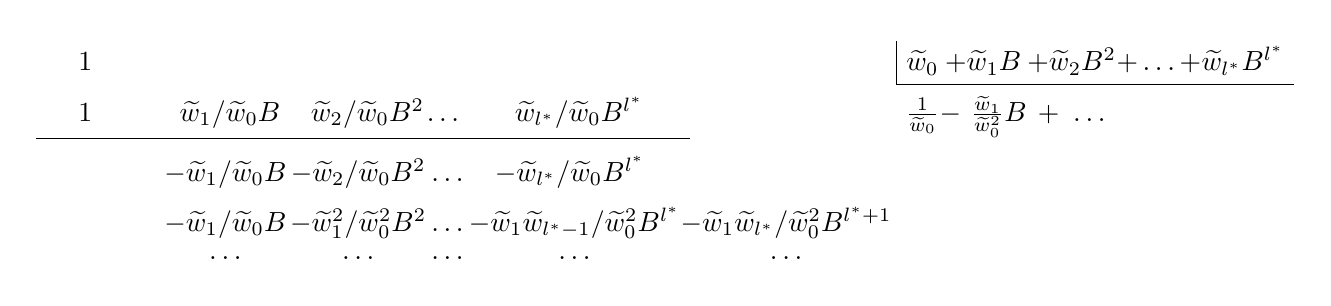
\begin{tikzpicture}
\matrix (a) [matrix of math nodes,column sep=-1.5ex]
{
% x^8 & x^7 & x^6 & x^5 & x^4 &
\phantom{w_1} 1\phantom{ / w_0 B}  & & & & & & & & 
\widetilde{w}_0 & +\widetilde{w}_1 B & + \widetilde{w}_2 B^2 & +  \ldots + & \widetilde{w}_{l^*} B^{l^*}\\
\phantom{w_1} 1\phantom{ / w_0 B}& \ \ \widetilde{w}_1 / \widetilde{w}_0 B \ & \ \ \widetilde{w}_2 / \widetilde{w}_0 B^2 & 
\ldots \ & \ \widetilde{w}_{l^*} / \widetilde{w}_0 B^{l^*} & \ & & & 
\frac{1}{\widetilde{w}_0} & - \ \frac{\widetilde{w}_1}{\widetilde{w}_0^2} B & + \ \ldots\\
& -\widetilde{w}_1 / \widetilde{w}_0 B & -\widetilde{w}_2 / \widetilde{w}_0 B^2 & \ldots & -\widetilde{w}_{l^*} / \widetilde{w}_0 B^{l^*} \ \\
& -\widetilde{w}_1 / \widetilde{w}_0 B & -\widetilde{w}_1^2 / \widetilde{w}_0^2 B^2 & \ldots & -\widetilde{w}_1 \widetilde{w}_{l^* - 1} / \widetilde{w}_0^2 
B^{l^*} & -\widetilde{w}_1 \widetilde{w}_{l^*} / \widetilde{w}_0^2 B^{l^* + 1} & \phantom{B^l}\\
& \ldots & \ldots & \ldots & \ldots & \ldots \\
};

\draw (a-1-9.north west)|-(a-1-13.south east);
\draw (a-2-1.south west)--(a-4-5.east|-a-2-2.south);
%\draw (a-4-2.south west)--(a-4-6.east|-a-4-4.south);
\end{tikzpicture}

\caption{First 2 terms of polynomial long division}
\label{fig:polyLongDiv}
\end{figure}

\section{Toy Project}
\label{sec:toyProjectFracDiff}
In the previous sections, the \textit{memory vs. stationarity} dilemma has 
been presented. On top of that, through fractional differentiation, 
stationarity has been achieved without totally giving up memory. Also, a 
method has been presented to differentiate and un-differentiate time series 
in a robust way.\\

That being said, the problem that this toy project attempts to solve will be 
presented. Given a time series $\{ y_t \}$, and $\Lambda_t$ representing all 
the values $\{ y_t \}$ has taken up to time $t$, the aim of this project is 
to give a forecast $\widehat{y}_{t + 1}$ given $\Lambda_t$. That way, by 
sequentially giving 1-day forecasts, a new time series will be generated.\\

To illustrate the effect fractional differentiation can have in the 
predicting power of a model, two models will be designed. One will have 
fully differentiated features and labels, and the other will use 
fractionally differentiated ones.\\

The last phase of the toy project will be computing prediction errors to 
compare the performance of the two models. 

\subsection{Synthetic data}
\label{sec:fracDiffToySyntheticData}
Striving to create a log-prices time series with memory, the generation was 
the following:

\begin{equation}
\label{eqn:tSeriesSynthetic}
	y_{t} = \frac{1}{5} \cdot \sum_{i = 1}^{5} y_{t - i} + 
	\mu + \epsilon_t \ \ (t \geq 6)
\end{equation}

where $\mu = 0.005$, $\epsilon_t \sim N(0,\ \sigma = 0.01)$ and 
$y_{1:5} = \{0.000,\ 0.075,\ 0.150,\ 0.225,\ 0.300\}$.\\

A few remarks:
\begin{itemize}
	\item $\left( 1 - \frac{1}{5} \sum_{k = 1}^5 B^k \right) y_t = 
	\phi (B) \ y_t = \mu + \epsilon_t$ has a unit root since 
	$z = 1$ 	is a root of $\phi(z)$. Therefore, $\{ y_t \}$ is not stationary 
	and will have to undergo some degree of differentiation.
	
	\item Rewriting \ref{eqn:tSeriesSynthetic}, one can obtain:
	\begin{align}	
	x_t := y_t - y_{t-1} = \frac{1}{5} \cdot \sum_{i = 1}^{5} (y_{t-i} - 
	y_{t-1}) + \mu + \epsilon_t = \frac{1}{5} \cdot \sum_{i = 2}^{5} (y_{t-i} 
	- y_{t-1}) + \mu + \epsilon_t = \nonumber \\ 
	= \frac{1}{5} \cdot \sum_{i = 2}^{5} (y_{t-i} - 	y_{t-i+1} + \ldots + 
	y_{t-2} - y_{t-1}) + \mu + \epsilon_t = \nonumber \\
	= -\frac{1}{5} \left( 	x_{t-4}	+ 2 x_{t-3} + 3 x_{t-2} + 4 x_{t-1} 
	\right) 	+ \mu + \epsilon_t \label{eqn:ARtoySynthetic}
	\end{align}
\end{itemize}

As it can be seen from equation \ref{eqn:tSeriesSynthetic}, in order to 
determine the value of $y_t$, it is crucial to know the preceding 5 values 
of the time series, while $x_t$ depends on the previous 4 values (see 
equation \ref{eqn:ARtoySynthetic}).\\

One big difference between $\{ y_t \}$ and  $\{ x_t \}$ is that the latter is 
stationary (checking that the roots of the characteristic equation lie 
outside the unit circle is left to the reader). However, both processes have 
the same Gaussian white noise ($\{ \epsilon_t \}$) which will be interesting 
to see how ML algorithms cope with it. To be specific, $\{ y_t \}$ goes to 
infinity as $t \rightarrow \infty$, while $\{ x_t \}$ is stationary, which 
means that as time passes $\{ y_t \}$ becomes less noisy.\\

As for the length of the time series, $\{ y_t \}$ will have 3000 
observations, and 15\% of them (450 obs.) will be saved for testing purposes.

\subsection{Fractional differentiation of $y_t$}
In figure \ref{fig:FFDSynthetic} and \ref{fig:FFDSyntheticZoom} the 
differentiated time series are shown. Note that the method used is the one 
defined previously: fixed-width window fractional differentation method 
(FFD). Also, in order to determine the minimnum $d^*$ that makes the time 
series stationary, figure \ref{fig:ADFSynthetic} and table 
\ref{tab:ADFStatistics} are presented (only training data has been used).\\

\begin{figure}[htbp]
	\centering
	\begin{minipage}{.5\textwidth}
  		\centering
  		\includegraphics[scale=0.25]{"\homeCTwo/img/FFDSynthetic"}
  		\caption{FFD of $y_t$ with $\tau = 1e-4$}
  		\label{fig:FFDSynthetic}
	\end{minipage}%
	\begin{minipage}{.5\textwidth}
  	\centering
  		\includegraphics[scale=0.25]{"\homeCTwo/img/FFDSyntheticZoom"}
  		\caption{FFD of $y_t$ (Zoomed in) with $\tau = 1e-4$}
  		\label{fig:FFDSyntheticZoom}
	\end{minipage}
\end{figure}

\begin{table}[htbp]
\centering
	\caption{ADF Test (with trend and drift) Statistics of $x_t^d$ - Train}
	\label{tab:ADFStatistics}
	\vspace{.1cm}
	\begin{tabular}{ |C{2cm}|C{2.5cm}|C{2cm}| }
		\hline
		d & Lag order ($p$) & ADF Statistic\\
		\hline
		0.00 & 13 & -3.130\\
		0.05 & 12 & -3.130\\
		0.10 & 12 & -3.430\\
		0.15 & 12 & -3.850\\
		0.20 & 12 & -4.254\\
		0.25 & 12 & -4.856\\
		0.30 & 12 & -5.352\\
		0.35 & 13 & -6.179\\
		0.40 & 13 & -6.939\\
		0.45 & 13 & -7.525\\
		0.50 & 13 & -8.141\\
		0.55 & 13 & -8.967\\
		0.60 & 13 & -9.819\\
		0.65 & 13 & -10.637\\
		0.70 & 13 & -11.515\\
		0.75 & 13 & -12.388\\
		0.80 & 13 & -13.265\\
		0.85 & 13 & -13.944\\
		0.90 & 13 & -14.684\\
		0.95 & 13 & -15.410\\
		1.00 & 13 & -16.077\\		
		\hline
	\end{tabular}
\end{table}	

\begin{figure}[htbp]
	\centering
	\includegraphics[scale=0.35]{"\homeCTwo/img/ADFSynthetic"}
	\caption{ADF Statistics of $x_t^d$ - Train}
	\label{fig:ADFSynthetic}
\end{figure}

Thus, now that it is known that $d^* = 0.2$, whenever the FFD time series is 
mentioned, the order of differentiation will be $d^*$.

\newpage

\subsection{Models}
With the purpose of evaluating how FFD works in this toy project, three 
models will be used:

\begin{enumerate}
	\item \textbf{Naive Model} (Benchmark): Simplest model than can be 
	built. It will predict $\widehat{y}_{t+1} = y_t$
	
	\item \textbf{FFD Model:} It will use $\{ x_t^{d^*} \}$ to predict 
	$\{ y_t \}$.
	
	\item \textbf{Returns Model:} It will use $\{ x_t \}$ 
	($x_t \equiv x_t^{1} = y_t - y_{t-1}$) to predict $\{ y_t \}$.
\end{enumerate}

The FFD and Returns models will be similar in the sense that they will use 
the same artificial neural network (ANN) structure and similar features. Both 
models will use the architecture seen in figure \ref{fig:fracDiffANN} but 
with 5 input units. Also, it is important to mention that they will use ELU 
(Exponential Linear Unit) as activation function.\\

Regarding the features and labels, due to the construction of the time 
series, the last 5 values will be used to predict the next one:
\begin{itemize}
	\item \textbf{Features:} $x_{t-5}^d$, $x_{t-4}^d$, $x_{t-3}^d$, 
	$x_{t-2}^d$ and $x_{t-1}^d$
	\item \textbf{Labels:} $x_{t}^d$
\end{itemize}

Lastly, recall that 450 observations out of 3000 will be used for testing 
purposes. This does not mean that 2550 observations will be used for 
training, since using the FFD method implies that the series will not be 
defined up to a point. That is caused by the fact that all observations 
should have the same amount of memory.

\subsection{Sequential forecasts}
\label{sec:toyProjectSeqForecast}
Considering that one is attempting to predict log-prices and differentiated 
features are being used, an emphasis should be put in the un-differentiation, 
which can be expressed (see equation \ref{eqn:series2Poly}) as:
\begin{equation*}
y_t = \sum_{k = 0}^{T - 1} c_k \cdot B^k \ x_t^d \hspace{.5cm} (T = 3000)
\end{equation*}

Noting $n_0$ as the time stamp where predictions start, the predicted time 
series will be defined sequentially as:
\begin{equation*}
	\widehat{y}_t = c_0 \cdot \widehat{x}_t^d + \sum_{k = 1}^{T - 1} c_k 
	\cdot B^k \ 	x_t^d = c_0 \cdot \widehat{x}_t^d + \sum_{k = 1}^{T - 1} c_k 
	\cdot x_{t - k}^d \hspace{.5cm} (t \geq n_0)
\end{equation*}

Here one needs to remember that, by definition, $x_{t}^d = 0$ for $t \leq 
0$.

\subsection{Results}
In the previous section, it has been shown how to obtain a new time series 
with the predictions. In order to compare the final time series in the test 
data set ($t \geq n_0$), three metrics will be used: Root-mean-square error 
(RMSE), Mean absolute percentage error (MAPE) and Median absolute deviation 
(MAD). The metrics mentioned will be defined after introducing the following 
parameters: $e_k = y_k - \widehat{y}_k$ and $\widetilde{e} = 
\text{median}(e_k)$.

\begin{equation*}
	\text{RMSE} = \sqrt{\frac{\sum_{k = n_0}^{T} (e_k)^2}
	{T - n_0 + 1}} 
\end{equation*}

\begin{equation*}
	\text{MAPE} = \frac{1}{T - n_0 + 1} \cdot \sum_{k = n_0}^T 
	\left| \frac{e_k}{y_k} \right| 
\end{equation*}

\begin{align*}
	\text{MAD} = \text{median}(|e_k - \widetilde{e}|)	
\end{align*}

With the metrics defined, the results in the test data set are the 
following (improvement over the benchmark is shown in parenthesis):
\begin{table}[htbp]
\centering
	\caption{Error metrics of the models considered - Test}
	\label{tab:MetricsToy}
	\vspace{.1cm}
	\begin{tabular}{ |C{2.5cm}|C{3.5cm}|C{2.5cm}|C{3.5cm}| }
		\hline
			 & FFD model & Naive model & Returns model\\
		\hline
		RMSE & 0.010184 (21.63\%) & 0.012995 & 0.013126 (-1.01\%)\\
		MAPE & 0.001608 (23.90\%) & 0.002113 & 0.002148 (-1.66\%)\\
		MAD  & 0.006606 (24.48\%) & 0.008747 & 0.009192 (-5.09\%)\\		
		\hline
	\end{tabular}
\end{table}

\begin{figure}[htbp]
\centering
	\includegraphics[scale=0.25]{"\homeCTwo/img/errorMetricsToy"}
	\caption{Error metrics of the models considered - Test}
	\label{fig:MetricsToy}
\end{figure}

\subsection{Conclusions}
From the results shown in table \ref{tab:MetricsToy} and figure 
\ref{fig:MetricsToy}, it can be implied that the FFD model has performed 
best across all error metrics. Also, the difference between the Naive and 
Returns Model is negligible, so it can be concluded that the Returns Model 
has not been able to detect the pattern behind the observations.\\

This goes to say that full differentiation is unnecessary. To be more 
specific, the FFD method has been able to retain some of the structure of 
$\{ y_t \}$. Consequently, as mentioned in section 
\ref{sec:fracDiffToySyntheticData}, it has not suffered as much from the 
Gaussian white noise so predictions are bound to be better.\\

The next step is to apply the same method to a real financial time series. 
Although this controlled project has been successful in an FFD sense, it 
remains to be seen whether fractional differentiation of financial time 
series helps with forecasts.

\section{Financial data}
\label{sec:fracDiffFinData}
The data used will be the log-prices of the S\&P500 from 2005-01-01 to 
2019-09-01. It will include the Open ($y_t^{\text{Open}}$), High 
($y_t^{\text{High}}$), Low ($y_t^{\text{Low}}$) and Close 
($y_t^{\text{Close}}$). That is, the log-price it opens/closes and the 
highest/lowest values during the daily trading session.\\

As in the project of section \ref{sec:toyProjectFracDiff}, the goal of the 
models will be to make a 1-day forecast. In particular, with the OHLC (Open, 
High, Low, Close) data of day $t$, the models will predict the value the 
stock closes at time $t + 1$. To do that, the features and labels 
will be the following:

\begin{itemize}
	\item \textbf{Features:} $y_t^{\text{Open}}$, $y_t^{\text{High}}$, 
	$y_t^{\text{Low}}$ and $y_t^{\text{Close}}$
	\item \textbf{Labels:} $y_{t + 1}^{\text{Close}}$
\end{itemize}

These features, as in \cite{gajda2020fractional}, have been chosen because 
they provide information at different times of the day. That is, they 
represent the daily state of the time series.

\subsection{Division Train/Test data sets}
The data will be divided into a training and test data set. The distribution 
is the following:

\begin{table}[htbp]
	\centering
	\caption{Division of Train/Test}
	\label{tab:trainTestFracDiff}
	\vspace{.1cm}
	\begin{tabular}{ |C{3.5cm}|C{2.5cm}|C{2.5cm}| }
		\hline
			 				& FFD model & Returns model\\
		\hline
		Start date (Train)	& 2006-10-06 & 2005-01-04\\
		End date (Train)		& 2017-07-12 & 2017-07-12\\
		\hline
		Start date (Test)	& 2017-07-14 & 2017-07-14\\
		End date (Test)		& 2020-08-28 & 2020-08-28\\
		\hline
		$n_{\text{Train}}$	& 2709 		 & 3152\\
		$n_{\text{Test}}$	& 788  		 & 788\\		
		\hline
	\end{tabular}
\end{table}

As it can be seen in table \ref{tab:trainTestFracDiff}, both the FFD and the 
Returns models have 788 observations in the test data set. However, in the 
train data set, the FFD has 443 fewer observations. This can be explained via 
equation \ref{eqn:FFD}, since by \textbf{setting a threshold} $\tau = 10^{-4}
$, an $l^*(\tau, d)$ exists such that the FFD is valid for $t \geq l^* +1$. 
In particular, in the case of returns $d = 1$, and thus, $l^*(\tau, d = 1) = 
1$ since the first observation does not have a preceding value.\\

Also note that $n_{\text{Test}}$ has been kept equal because the error 
metrics will be evaluated in this data set. Consequently, the conditions 
should be the same to avoid misleading results.

\section{Models}
As in section \ref{sec:toyProjectFracDiff}, three models will be used: 
\textbf{Naive}, \textbf{FFD} and \textbf{Returns} model. The features will 
be the corresponding time series shown in section \ref{sec:fracDiffFinData}, 
but differentiated. To be specific, the FFD model will use the fractionally 
differentiated features with the minimum order ($d^* = 0.25$) that makes the 
4 OHLC time series stationary (in training). Conversely, the 
\textbf{Returns} model will use fully differentiated features ($d = 1$).\\

The \textbf{FFD} and \textbf{Returns} models will use an ANN with the 
structure seen in figure \ref{fig:fracDiffANN}. As in section 
\ref{sec:toyProjectFracDiff}, the activation function will be the 
Exponential Linear Unit (ELU).

\begin{figure}[htbp]
	\centering
	\includegraphics{"\homeCTwo/img/fracDiffANN"}
	\caption{ANN used in the FFD and Returns Models}
	\label{fig:fracDiffANN}
\end{figure}

\section{Data normalization}
As a means to provide features to the neural network with the same range, 
all 4 features have been normalized:

\begin{equation*}
	z_t = \frac{y_t - y_{\text{min}}}{y_{\text{max}} - y_{\text{min}}}
\end{equation*}

It should be pointed out that $y_{\text{max}}$ and $y_{\text{min}}$ have 
been computed in the \textbf{train} data set. It is extremely important to 
consider this, because if one were to use the maximum/minimum of the whole 
data set, look-ahead bias would have occurred. To be more specific, if the 
test observations started at time $t_0$ and the time stamp when the maximum 
is achieved is $t_0 + m > t_0$, then the forecast at time $t_0$ would have 
used information from $t_0 + m$, which is impossible.\\

That being said, in the train data set, $z_t \in [0, 1]$, while in the test 
data set, features are not guaranteed to be in $I = [0, 1]$. However, 
working under the assumption that the complete time series is stationary, 
values can not be far off.\\

It should also be brought up that since labels are not normalized, the 
predicted values will not have to undergo ``un-normalization''.

\section{Results}
\label{sec:resultsFFD}
As in section \ref{sec:toyProjectSeqForecast}, the sequential forecasts have 
been calculated and the final result is 3 time series, which are forecasts 
of the close of the S\&P500:

\begin{align*}
	y_t^{\text{Naive}} \hspace{.51cm} (n_0 + 1 \leq t \leq T)\\
	y_t^{\text{FFD}} \hspace{.64cm} (n_0 + 1 \leq t \leq T)\\
	y_t^{\text{Returns}} \hspace{.25cm} \hfill (n_0 + 1 \leq t \leq T)\\
\end{align*}

Where $t = n_0$ is the time stamp that marks the start of the test data set. 
Therefore, the prediction will be of the log-price close of time $t + 1 = 
n_0 + 1$

\begin{table}[htbp]
\centering
	\caption{Error metrics of the models considered in the Test data set}
	\label{tab:MetricsFFD}
	\begin{tabular}{ |C{2.5cm}|C{3.5cm}|C{2.5cm}|C{3.5cm}| }
		\hline
			 & FFD model 	& Naive model 	& Returns model\\
		\hline
		RMSE & 0.0187200 (-0.78\%) & 0.0185758 & 0.0181539 (2.27\%)\\
		MAPE & 0.0017909 (-1.91\%) & 0.0017573 & 0.0017179 (2.24\%)\\
		MAD  & 0.0047790 (-6.85\%) & 0.0044728 & 0.0044403 (0.73\%)\\
		\hline
	\end{tabular}
\end{table}

In table \ref{tab:MetricsFFD} the error metrics for the three models 
considered are shown, as well as the improvement over the Naive model 
(displayed in parentheses). For a graphical representation refer to figure
\ref{fig:MetricsFFD}. In addition, figures \ref{fig:resultsFFD1}, 
\ref{fig:resultsFFD2} and \ref{fig:resultsFFD3} present the forecasted time 
series for different periods of time.

\begin{figure}[htbp]
	\centering
	\begin{minipage}{.5\textwidth}
  		\centering
		\includegraphics[scale=0.25]{"\homeCTwo/img/errorMetricsFFD"}
		\caption{Error metrics of the models considered - Test}
		\label{fig:MetricsFFD}
	\end{minipage}%
	\begin{minipage}{.5\textwidth}
  		\centering
		\includegraphics[scale=0.25]{"\homeCTwo/img/resultsFFD1"}
		\caption{Forecasted time series - Test}
		\label{fig:resultsFFD1}
	\end{minipage}
\end{figure}


\begin{figure}[htbp]
	\centering
	\begin{minipage}{.5\textwidth}
  		\centering
  		\includegraphics[scale=0.25]{"\homeCTwo/img/resultsFFD2"}
  		\caption{Results 2018-07/2018-10}
  		\label{fig:resultsFFD2}
	\end{minipage}%
	\begin{minipage}{.5\textwidth}
  		\centering
  		\includegraphics[scale=0.25]{"\homeCTwo/img/resultsFFD3"}
  		\caption{Results 2019-03/2019-06}
  		\label{fig:resultsFFD3}
	\end{minipage}
\end{figure}

\newpage

\section{Conclusions}
This chapter has explored how fractional differentiation can be applied to 
financial data. Through a toy project it was observed that in a process that
had memory, i.e. future values depended on the past, one could achieve better 
forecasts by using fractionally differentiated features instead of a full 
differentiation.\\

However, when it came to financial data the results were not as one would 
have expected. As shown in section \ref{sec:resultsFFD}, the FFD model was 
the worst performer among the three models. In particular, it should be 
pointed out that the metrics of the FFD model were slightly worse than the 
ones of 	the Naive model. In contrast, the performance of the Returns model 
was a bit better than the Naive.\\

On the grounds that the performance was so similar, the differences are 
attributed to randomness. That is, one should not expect the FFD or Returns 
model to outperform or underperform the Naive Model, indicating that the 
features used were not useful at making 1-day forecasts.\\

All in all, this chapter has encountered a similar situation than in 
meta-labeling. Fractional differentiation is a tool that should be used 
whenever one knows that the underlying time series has memory. That is, it is 
not a plug and play solution and should only be implemented if the current 
value of the time series relative to previous ones (memory) is helpful at 
giving forecasts.

\chapter{Data parsing as bars}
\label{chapterDataParsing}
The previous chapters used low frequency data. In particular, daily data was 
used which just means that after every trading day a single observation is 
gathered. On the other side of the spectrum rests high frequency data, which 
can be viewed as the purest form of financial data.\\

However, raw data does not mean that everything will work better. To feed 
this data to ML algorithms, it must be preprocessed in a way that 
superfluous information is discarded and useful parts are kept.\\

Before diving into the actual data manipulation, a brief explanation will be 
given to understand better where the term ``data bars'' come. As López de 
Prado states in~\cite{AdvFML}, most ML algorithms assume a table 
representation of the extracted data and the tables' rows are often referred 
by practitioners as ``bars''.

\section{Data bars}
In section \ref{sec:highFrequencyData} of chapter \ref{chapterIntroFinDat}, 
it was seen that raw financial data comes in ticks, and thus, inhomogenous 
in time. In order to structure data, samples of the price will be recorded 
whenever a certain event happens (time elapsed, price change, etc.). In 
consequence, different events will give rise to different type of bars.\\

A useful concept that will help understand how data bars arose is the 
concept of stochastic clock, proposed by Clark 
in~\cite{clark1973subordinated}. This clock will only ``show the time'' when 
certain events happen. For instance, a volume clock will only show the time 
when $M_{\text{volume}}$ units are exchanged. Hence, volume bars will be 
recorded whenever the volume clock ``shows the time''.\\

In the following subsections, the bars that Marcos López de Prado designated 
as standard in \cite{AdvFML} will be presented. 

\subsection*{Time bars}
These bars consist of sampling the price every $M_{\text{time}}$ minutes 
(e.g. every 1, 5, 30 minutes or longer). Note that daily data lays in this 
category since it records the price of an asset once a day.\\

One of the drawbacks of time bars is the fact that they ignore periods of 
high activity. That is, if one was sampling every 30 minutes and the bulk of 
trading occurred during the first and last 15 minutes of the trading 
session, then information would be lost.

\subsection*{Tick Bars}
As the name implies, the sampling will occur every certain amount of ticks 
($M_{\text{ticks}}$). Since ticks are directly related with transactions, 
during periods of high activity more samples will be gathered.\\

The problem with sampling data using ticks is the lack of control over the 
number of stocks traded. To put it another way, if one wanted to buy 5 
stocks and there were 5 separate offers of size 1 that matched, then the 
whole operation would count as 5 transactions. However, if there was an offer 
of size 5 that matched, it would be recorded as 1 transaction, even though 
the same number of stocks have been exchanged.\\

That is why López de Prado states in~\cite{AdvFML} that order fragmentation 
introduces arbitrariness in the number of ticks.

\subsection*{Volume bars}
Volume bars will sample the price every time $M_{\text{volume}}$ stocks are 
exchanged. This will certainly help with the issue outlined with tick bars. 
In this type of bars the amount of transactions will not matter since it 
only cares about the actual amount of securities traded.\\

Also, note that one of the great virtues of volume bars is the fact that 
they will sample the price correctly in moments of high activity. In 
particular, whenever a lot of stocks are traded, plenty of bars will be 
recorded, while in a low activity environment few bars will be gathered.

\subsection*{Dollar bars}
Before introducing these bars one should know what dollar volume is: 
$d_t := v_t \cdot p_t$. At first glance, one could infer that sampling every 
time a certain dollar volume ($M_{\text{dollar}}$) is traded will lead to 
bars similar to volume ones.\\

That is true to a certain extent because if $p_t$ stays fairly constant, 
then accounting for a constant, they will sample in a similar fashion. 
However, if the stock presents high volatility, volume bars will under 
sample periods of high prices. To be specific, dollar bars can distinguish 
300 stocks being exchanged at 80\$ ($ d_t = 24,000\$ $) rather than at 70\$ 
($ d_t = 21,000\$ $).\\

\section{Data}
The security that will be used for this chapter is called \textbf{IVE}, 
which trades in the NYSE (New York Stock Exchange) Arca market. This asset 
tracks the S\&P500, which is an index that comprises the 500 most important 
US stocks.\\

Having said that, the data used will be the tick data of IVE from 2013-01-02 
to 2013-12-31. It contains 550,697 rows that include information on: price, 
bid, ask, and volume. To get an idea of the general structure of the data 
used, refer to table \ref{tab:tickData} which shows a few ticks from day 
2013-01-02.

\section{Sampling}
Having presented the tick data that will be used, the next step is 
determining the hyperparameters $M_{\text{ticks}},\ M_{\text{volume}},\ 
M_{\text{dollar}}$ and $M_{\text{time}}$, which are responsible of the 
sample gathering. Once the samples are collected the daily average of bars 
($\bar{n}^{\text{daily}}$) will be calculated. Hence, every $M$ directly 
determines $\bar{n}^{\text{daily}}$.\\

Before showing the values of $M$ used, one should bear in mind that 
processing the huge dataset and creating the bars takes a considerable 
amount of time ($\approx$ 3 hrs). Therefore, ``brute force'' is not feasible 
to choose the values of $M$. However, what has been done is the following:

\begin{itemize}
	\item Choose a sensible $M$. For example, López de Prado 
	in~\cite{volumeClock} uses $\frac{1}{50}$ of the average daily volume as
	$M_{\text{volume}}$.

	\item Shift $M$ until the fitted pdf of log-returns resembles more of a 
	normal pdf (see section \ref{sec:normalLogRet} for further details).
\end{itemize}

Having said that, the final hyperparameters chosen are shown in table
\ref{tab:samplingM}.

\newpage

\begin{table}[htbp]
\caption{Sampling hyperparameters}
\label{tab:samplingM}
\centering
\begin{tabular}{ |C{2cm}|C{2cm}|C{2cm}|C{2cm}|C{2cm}| }
	\hline
	 				& Tick & Volume & Dollar & Time\\
	\hline
	$M$ & 60 ticks & 8,000 stocks & 800,000\$ & 8 min.\\
	$\bar{n}^{\text{daily}}$ & 36.42 & 73.77 & 49.20 & 49.93\\
	\hline
\end{tabular}
\end{table}

Figure \ref{fig:dataBars} shows three trading days and the samples that were 
extracted using tick, volume, dollar and time bars. Additionally, in figure 
\ref{fig:intradayDeformed} the samples of day 2013-07-10 are presented. This 
last image is really important because it symbolizes the data bars via their 
internal clock, i.e., one unit in the x-axis represents the occurrence of a 
certain event (stocks exchanged, ticks, etc.).\\

Furthermore, since it is of the utmost importance to understand how sampling 
occurs, a few remarks on figures \ref{fig:dataBars} and 
\ref{fig:intradayDeformed} will be made:
\begin{itemize}
	\item Tick bars, although not equally spaced as time bars, seem to be 
	more distributed as time passes compared to volume and dollar bars.
	
	\item Volume and dollar samples are concentrated on periods of high 
	volatility (downswings and upswings).
	
	\item In figure \ref{fig:intradayDeformed} it can be seen that tick, 
	volume and dollar bars undersample periods where the price goes 
	sideways, while they oversample the period from 14:00 to 15:00, where 
	the bulk of activity was observed.
\end{itemize}

\begin{figure}[htbp]
	\centering
	\begin{subfigure}{.5\textwidth}
		\centering
		\includegraphics[scale=.25]{img/dataBars/sampling1}
	\end{subfigure}%
	\begin{subfigure}{.5\textwidth}
		\centering
		\includegraphics[scale=.25]{img/dataBars/sampling2}
	\end{subfigure}%

	\vspace{.4cm}

	\begin{subfigure}{\textwidth}
		\centering
		\includegraphics[scale=.25]{img/dataBars/sampling3}
	\end{subfigure}
	
	\caption{Tick, volume, dollar and time bars}
	\label{fig:dataBars}
\end{figure}

\begin{figure}[htbp]
	\centering
	
	\begin{subfigure}{\textwidth}
		\centering
		\includegraphics[scale=.5]{img/dataBars/regularZoom}
		\caption{Tick data}
	\end{subfigure}%
	
	\vspace{.4cm}
	
	\begin{subfigure}{.5\textwidth}
		\centering
		\includegraphics[scale=.25]{img/dataBars/tickZoom}
		\caption{Tick bars}
	\end{subfigure}%
	\begin{subfigure}{.5\textwidth}
		\centering
		\includegraphics[scale=.25]{img/dataBars/volumeZoom}
		\caption{Volume bars}
	\end{subfigure}%

	\vspace{.4cm}

	\begin{subfigure}{.5\textwidth}
		\centering
		\includegraphics[scale=.25]{img/dataBars/dollarZoom}
		\caption{Dollar bars}
	\end{subfigure}%
	\begin{subfigure}{.5\textwidth}
		\centering
		\includegraphics[scale=.25]{img/dataBars/timeZoom}
		\caption{Time bars}
	\end{subfigure}%
	
	\caption{Sampling of 2013-07-10 tick data via tick, volume, dollar and 
	time bars}
	\label{fig:intradayDeformed}
\end{figure}

\newpage

\section{Normality of log-returns}
\label{sec:normalLogRet}
Once the samples have been gathered, it is time to compute log-returns and 
analyze their distribution. López de Prado argues in~\cite{volumeClock} that 
the time transformation induced by data bars allows a partial recovery of 
Normality.\\

However, after normalizing data, i.e. transform it such that it has a 
mean of 0 and a standard deviation of 1, the pdfs are far from normal (see 
figures \ref{fig:pdfLogReturns} and \ref{fig:QQPlotsDataBars}). Even after 
plotting the pdf of a $N(\mu = 0, \sigma = 0.5)$, it can be seen that the 
pdfs of all of the bars considered are heavy tailed.

\begin{figure}[htbp]
	\centering
	\includegraphics[scale=.35]{img/dataBars/pdfLogReturns}
	\caption{Fitted pdf of log-returns from data bars}
	\label{fig:pdfLogReturns}
\end{figure}

As a last comment on normality, note that in figure 
\ref{fig:QQPlotsDataBars} the QQ Plots of tick, volume and dollar bars have 
more pronounced tails than time bars. This is attributed to oversampling 
periods of high volatility, which by definition imply drastic changes in 
prices.

\begin{figure}[htbp]
	\centering

	\begin{subfigure}{.5\textwidth}
		\centering
		\includegraphics[scale=.25]{img/dataBars/tickQQPlot}
		\caption{Tick bars}
	\end{subfigure}%
	\begin{subfigure}{.5\textwidth}
		\centering
		\includegraphics[scale=.25]{img/dataBars/volumeQQPlot}
		\caption{Volume bars}
	\end{subfigure}%

	\vspace{.4cm}

	\begin{subfigure}{.5\textwidth}
		\centering
		\includegraphics[scale=.25]{img/dataBars/dollarQQPlot}
		\caption{Dollar bars}
	\end{subfigure}%
	\begin{subfigure}{.5\textwidth}
		\centering
		\includegraphics[scale=.25]{img/dataBars/timeQQPlot}
		\caption{Time bars}
	\end{subfigure}%
	
	\caption{QQ Plots of data bars}
	\label{fig:QQPlotsDataBars}
\end{figure}

\newpage

\section{Statistical analysis of bars}

With the aim of understanding better the behavior of data bars some 
parameters have been calculated and presented in table 
\ref{tab:statAnalysisDataBars}, giving rise to the following remarks:

\begin{itemize}
	\item Regarding $\text{ACF}_1$, the auto correlation function of lag 1, 
	time bars are the only type of bars that have a statistically 
	significant one.
	
	\item $\text{Var}[\widetilde{\sigma}^2]$ is the variance of 
	$\widetilde{\sigma}^2$, where the latter is the square of monthly 
	volatility. Therefore, a small variance will mean that volatility tends 
	to stay fairly constant month over month. This is what happened with 
	volume bars, whose variation of monthly volatility is the lowest.
	
	\item $\bar{n}^{\text{weekly}}$, the average number of bars in a week 
	shows that tick bars have the fewest, dollar and time bars really 
	similar numbers, and volume bars having the most.
	
	\item $\text{SD}[n^{\text{weekly}}]$, the standard deviation of the 
	number of weekly bars, shows that time bars are the most stable ones. 
	This should not be a surprise because being equally time spaced makes 
	them deterministic, with the only variability introduced via weeks with 
	holidays. Apart from that, tick and dollar bars follow along and volume 
	bars are the ones that display the most variability.
\end{itemize}

\begin{table}[htbp]
\caption{Statistical analysis of bars}
\label{tab:statAnalysisDataBars}
\centering
\begin{tabular}{ |C{3cm}|C{3cm}|C{3cm}|C{3cm}|C{3cm}| }
	\hline
	 				& Tick & Volume & Dollar & Time\\
	\hline
	%Jarque-Bera Statistic & 191,732.4 & 838,289.1 & 512,942.7 & 696,297.4\\
	$\text{ACF}_1$ & -0.01090561 & -0.01225259 & -0.01482256 & 
	-0.06833088\\
	$\text{Var}[\widetilde{\sigma}^2]$ & $2.936431 \cdot 10^{-13}$ &   
	$7.139122 \cdot 10^{-14}$ & $1.054108 \cdot 10^{-13}$ & 
	$1.618769 \cdot 10^{-13}$\\
	$\bar{n}^{\text{weekly}}$ & 173.1509 & 303.1698 & 233.9245 & 237.3962\\
	$\text{SD}[n^{\text{weekly}}]$ & 63.95744 & 101.94866 & 73.20699 
	& 31.19069\\
	\hline
\end{tabular}
\end{table}

To complement the information given in table \ref{tab:statAnalysisDataBars}, 
figure \ref{fig:weeklyBarCounts} shows the normalized (to a [0,1] interval) 
number of weekly bars.

\begin{figure}[htbp]
	\centering
	\includegraphics[scale=.35]{img/dataBars/weeklyBarCounts}
	\caption{Normalized weekly bar counts}
	\label{fig:weeklyBarCounts}
\end{figure}

\section{Results}
\label{sec:ARResults}
Having presented the method to create data bars, the obvious question is: 
does sampling the price time series in a different way than time bars give a 
predictive edge?\\

In an attempt to shed some light on the previous question a simple 
autoregressive (AR) model will be used to fit the log-returns obtained via 
tick, volume, dollar and time bars:

\begin{equation*}
	r_k = c + \sum_{i = 1}^{p} \theta_i r_{k - i} + \epsilon_k
\end{equation*}

Note that $r_k$ is no longer indexed via $t$ since it is no longer a time 
series, but a sequence. Additionally, the model order ($p$) will be 
determined with the R package stats \cite{RStats}, which uses the Akaike 
Information Criterion (AIC). This criterion is used to compare different 
models, in this case, different lags $p$.\\

As the datasets obtained with the bars are different, the training data will 
be the whole dataset except the \textbf{last 150 observations}. This number 
is fixed instead of a percentage because datasets have different sizes.\\

The forecasts will be given in a sequential manner. That is, if $N$ is the 
number of bars in the dataset, the model will be trained on the first 
$N - 150$ bars and give a 1-bar forecast ($\widehat{r}_k$). Then, it will be 
trained on the first $N - 150 + 1$ and then give a 1-bar forecast and so on.
\\

Lastly, considering that the datasets are different, an objective way to 
compare the errors $e_k = \widehat{r}_k - r_k$ is the Mean Absolute 
Percentage Error (MAPE):

\begin{equation*}
	\text{MAPE} = \frac{1}{150} \cdot \sum_{k = N - 150 + 1}^N 
	\left| \frac{e_k}{r_k} \right|
\end{equation*}

Note that the metrics used in previous chapters (RMSE, MAD) are 
inappropriate because they are not comparable over different datasets.
\begin{table}[htbp]
\caption{AR results}
\label{tab:ARDataBars}
\centering
\begin{tabular}{ |C{3cm}|C{2cm}|C{2cm}|C{2cm}|C{2cm}| }
	\hline
	 				& Tick & Volume & Dollar & Time\\
	\hline
	Lag ($p$) & 0 & 1 & 10 & 2\\
	MAPE & 1.187730 & 1.129902 & 1.134345 & 2.041313\\
	Improvement & 41.82\% & 44.64\% & 44.43\% & 0\% \\
	\hline
\end{tabular}
\end{table}

As for the results, refer to table \ref{tab:ARDataBars}, which shows the 
chosen lag, the model's MAPE and the improvement on MAPE over the time bar 
model (\textbf{benchmark}). The most striking points are:

\begin{itemize}
	\item The performance of the time model is the worst, with a MAPE of 
	2.04

	\item The tick model, even though the lag used is 0 which means that it 
	predicts a constant, achieves a better MAPE than the time model.
	
	\item The volume and dollar models achieve similar results 
	($\approx 44\%$ improvement) but the complexity of the dollar model is 
	much higher ($p = 10$). Thus, the volume model is preferred.
\end{itemize} 

\section{Conclusions}
This chapter has introduced a useful technique to sample financial data. 
Although it was not possible to recover normality of log-returns through 
this new sampling method, the autoregressive models considered in section 
\ref{sec:ARResults} delivered promising results. The next step would be to 
develop ML Models, that together with other features, would help predict the 
direction of the stock in a determined bar horizon.\\

Additionally, it also remains as future work to design a strategy that is 
able to incorporate data bars. High frequency trading is extremely difficult 
to replicate in an artificial environment since one has to account for 
information lag, order execution, etc. Apart from that, trading with volume 
bars is challenging since it introduces a ``stochastic clock''. That is, if 
one wants to  open a position and the algorithm determines that it should 
be closed after $m$ bars, ones does not know when that event is going to 
happen.

\chapter{Conclusions and future work}
\label{chapterConclFutWork}
% Paragraph 1
% Overview of the methods - connection with the abstract
The goal of this thesis was to explore meta-labeling, fractional 
differentiation and data parsing as bars in the financial context with the 
purpose of determining if they were useful at delivering better forecasts 
and/or higher risk-adjusted returns. In order to fulfill this goal, three 
independent chapters have been presented, which have analyzed the techniques 
mentioned.\\

% Paragraph 2
% Conclusion of each method
First of all, after studying meta-labeling thoroughly it can be concluded 
that this technique is very specific in the sense that it needs a certain 
environment to deliver better results. To be precise, as it was seen via the 
\textit{coin flip} correction, to deliver higher Sharpe Ratios it needed a 
primary model that was good by itself, Sharpe Ratio wise. As the primary 
models developed did not achieve satisfactory Sharpe Ratios, the results 
mentioned before were not realized. Therefore, meta-labeling should only be 
used if one is confident that their primary model is good but needs minimal 
tweaking.\\

Secondly, fractional differentiation was useful at providing a framework to 
achieve stationarity without losing memory in time series. However, it did 
not translate into better forecasts. This is attributed to financial data, 
where memory was determined to not be highly relevant at giving predictions.
\\

Lastly, the sampling technique known as data parsing as bars was helpful at 
giving better forecasts. It evidenced that in high frequency data, activity 
is more important than time.\\

% Paragraph 3
Furthermore, it should be pointed out that there is still room for 
improvement. The data used in this thesis was centered around time series. 
However, in Finance there are alternative data sources such as financial 
news, macroeconomic data, FOREX, etc. It remains to be seen how these could 
have improved the performance of the Machine Learning models.\\

% Paragraph 4
Regarding future work that might spin off of this thesis, it is important to 
mention the design of high frequency trading strategies. Having explored 
sampling of high frequency data, it is natural to continue working with this 
type of data, which is the perfect environment to further test 
meta-labeling, fractional differentiation ...\\

% Paragraph 5
On the personal side, the author has learned that using Machine Learning in 
Finance is not a matter of what but when. One can have the most promising 
techniques but fail to deliver results due to not applying the model to the 
correct data set. In part, this is what happened in the meta-labeling and 
fractional differentiation chapters, which in financial data failed to 
deliver the results observed in the toy projects.\\

% Paragraph 6
As a final note, it should be acknowledged that this thesis has been 
extremely useful to learn concepts that the author was oblivious of. That is, 
time series analysis, high frequency financial data and Machine Learning 
models. Also, this work has been an excellent introduction to academic 
research, since it has laid the foundations of the author's academic career, 
which he intends to continue in the coming years.

\newpage
\bibliography{references}

\begin{table}[htbp]
\caption{Tickers of the GMVP portfolio}
\label{table:tickers}
\centering
\begin{tabular}{ |C{2cm}|C{2cm}|C{2cm}|C{2cm}|C{2cm}|C{2cm}| }
	\hline
	MMM & ABT & ABBV & ABMD & ACN & ATVI\\
	ADBE & AMD & AAP & AES & AFL & A\\
	APD & AKAM & ALK & ALB & ARE & ALXN\\
	ALGN & ALLE & LNT & ALL & GOOGL & GOOG\\
	MO & AMZN & AMCR & AEE & AAL & AEP\\
	AXP & AIG & AMT & AWK & AMP & ABC\\
	AME & AMGN & APH & ADI & ANSS & ANTM\\
	AON & AOS & APA & AIV & AAPL & AMAT\\
	APTV & ADM & ANET & AJG & AIZ & T\\
	ATO & ADSK & ADP & AZO & AVB & AVY\\
	BKR & BLL & BAC & BK & BAX & BDX\\
	BRK.B & BBY & BIO & BIIB & BLK & BA\\
	BKNG & BWA & BXP & BSX & BMY & AVGO\\
	BR & BF.B & CHRW & COG & CDNS & CPB\\
	COF & CAH & KMX & CCL & CARR & CTLT\\
	CAT & CBOE & CBRE & CDW & CE & CNC\\
	CNP & CERN & CF & SCHW & CHTR & CVX\\
	CMG & CB & CHD & CI & CINF & CTAS\\
	CSCO & C & CFG & CTXS & CLX & CME\\
	CMS & KO & CTSH & CL & CMCSA & CMA\\
	CAG & CXO & COP & ED & STZ & COO\\
	CPRT & GLW & CTVA & COST & CCI & CSX\\
	CMI & CVS & DHI & DHR & DRI & DVA\\
	DE & DAL & XRAY & DVN & DXCM & FANG\\
	DLR & DFS & DISCA & DISCK & DISH & DG\\
	DLTR & D & DPZ & DOV & DOW & DTE\\
	DUK & DRE & DD & DXC & EMN & ETN\\
	EBAY & ECL & EIX & EW & EA & EMR\\
	ETR & EOG & EFX & EQIX & EQR & ESS\\
	EL & ETSY & EVRG & ES & RE & EXC\\
	EXPE & EXPD & EXR & XOM & FFIV & FB\\
	FAST & FRT & FDX & FIS & FITB & FE\\
	FRC & FISV & FLT & FLIR & FLS & FMC\\
	F & FTNT & FTV & FBHS & FOXA & FOX\\
	BEN & FCX & GPS & GRMN & IT & GD\\
	GE & GIS & GM & GPC & GILD & GL\\
	GPN & GS & GWW & HAL & HBI & HIG\\
	HAS & HCA & PEAK & HSIC & HSY & HES\\
	HPE & HLT & HFC & HOLX & HD & HON\\
	HRL & HST & HPQ & HUM & HBAN & HII\\
	IEX & IDXX & INFO & ITW & ILMN & INCY\\
	IR & INTC & ICE & IBM & IP & IPG\\
	IFF & INTU & ISRG & IVZ & IPGP & IQV\\
	IRM & JKHY & J & JBHT & SJM & JNJ\\
	JCI & JPM & JNPR & KSU & K & KEY\\
	KEYS & KMB & KIM & KMI & KLAC & KHC\\
	KR & LB & LHX & LH & LRCX & LW\\
	LVS & LEG & LDOS & LEN & LLY & LNC\\
	LIN & LYV & LKQ & LMT & L & LOW\\
	LYB & MTB & MRO & MPC & MKTX & MAR\\
	MMC & MLM & MAS & MA & MKC & MXIM\\
	MCD & MCK & MDT & MRK & MET & MTD\\
	MGM & MCHP & MU & MSFT & MAA & MHK\\
	\hline
\end{tabular}
\end{table}

\begin{table}[htbp]
\caption{Tickers (continued) of the GMVP portfolio}
\label{table:tickersCont}
\centering
\begin{tabular}{ |C{2cm}|C{2cm}|C{2cm}|C{2cm}|C{2cm}|C{2cm}|  }
	\hline
	TAP & MDLZ & MNST & MCO & MS & MOS\\
	MSI & MSCI & MYL & NDAQ & NOV & NTAP\\
	NFLX & NWL & NEM & NWSA & NWS & NEE\\
	NLSN & NKE & NI & NSC & NTRS & NOC\\
	NLOK & NCLH & NRG & NUE & NVDA & NVR\\
	ORLY & OXY & ODFL & OMC & OKE & ORCL\\
	OTIS & PCAR & PKG & PH & PAYX & PAYC\\
	PYPL & PNR & PBCT & PEP & PKI & PRGO\\
	PFE & PM & PSX & PNW & PXD & PNC\\
	POOL & PPG & PPL & PFG & PG & PGR\\
	PLD & PRU & PEG & PSA & PHM & PVH\\
	QRVO & PWR & QCOM & DGX & RL & RJF\\
	RTX & O & REG & REGN & RF & RSG\\
	RMD & RHI & ROK & ROL & ROP & ROST\\
	RCL & SPGI & CRM & SBAC & SLB & STX\\
	SEE & SRE & NOW & SHW & SPG & SWKS\\
	SLG & SNA & SO & LUV & SWK & SBUX\\
	STT & STE & SYK & SIVB & SYF & SNPS\\
	SYY & TMUS & TROW & TTWO & TPR & TGT\\
	TEL & FTI & TDY & TFX & TER & TXN\\
	TXT & TMO & TIF & TJX & TSCO & TT\\
	TDG & TRV & TFC & TWTR & TYL & TSN\\
	UDR & ULTA & USB & UAA & UNP & UAL\\
	UNH & UPS & URI & UHS & UNM & VFC\\
	VLO & VAR & VTR & VRSN & VRSK & VZ\\
	VRTX & V & VNO & VMC & WRB & WAB\\
	WMT & WBA & DIS & WM & WAT & WEC\\
	WFC & WELL & WST & WDC & WU & WRK\\
	WY & WHR & WMB & WLTW & WYNN & XEL\\
	XRX & XLNX & XYL & YUM & ZBRA & ZBH\\
	ZION & ZTS & & & & \\
	\hline
\end{tabular}
\end{table}

\end{document}
